\section{Tensor Decompositions}\label{chapter:tensor-decomposition}
Working with high-order tensors is computationally expensive because the number of elements grows exponentially with the tensor's order. Tensor decompositions have emerged as powerful and efficient tools to address this issue.
Similar to matrix factorizations, tensor decompositions break down a high-order tensor into smaller components with lower-order and fewer entries, making computations more tractable. However, the notion of the rank of a matrix can be extended in various ways for tensors, each of them associated with a different factorization/decomposition model.
In this chapter, we introduce the most well-known tensor decomposition models.
\subsection{CANDECOMP/PARAFAC~(CP) Decomposition}\label{sec:cp-decomposition}
The CP decomposition~\citep{hitchcock1927expression} of an $N$-th order tensor $\At\in\RR^{d_1\times\cdots\times d_N}$  decomposes $\At$ as the sum of a finite number of rank-one tensors. Equivalently, it is a linear combination of $R$ rank-one tensors where $R$ is called the  rank of the decomposition: 
$$\At = \sum_{r=1}^R \ab^{(r)}_1\outprod\dots\outprod\ab^{(r)}_N ,$$
where $\ab^{(1)}_n,\dots,\ab^{(R)}_n\in\RR^{d_n}$ for each $n\in [N]$.

By grouping all the vectors $\ab^{(r)}_n$ in factor matrices,
\[\Ab_1 = {\begin{pmatrix}
\ab^{(1)}_1 & \dots & \ab^{(R)}_1 \\
\end{pmatrix}}{\in\RR^{d_1\times R}}, \dots ,\Ab_N = {\begin{pmatrix}
\ab^{(1)}_N & \dots & \ab^{(R)}_N \\
\end{pmatrix}}{\in\RR^{d_N\times R}}, \]
the CP decomposition is concisely noted as $\At = \CP{\Ab_1,\cdots,\Ab_N}$.

In tensor networks, a CP decomposition $\At = \CP{\Ab,\Bb,\Cb}$ is represented by
$$
\begin{tikzpicture}[baseline=\baseline]
    \tikzset{tensor/.style = {minimum size = 0.5cm,shape = circle,thick,draw=black,inner sep = 0pt}, edge/.style   = {thick,line width=.4mm},every loop/.style={}}
    \def\y{0}
    \def\x{0}
    \node[tensor,fill=green!50!red!50!white] (A) at (\x,\y){\scalebox{0.85}{$\At$}};
    \draw[edge] (\x+0.25,\y) -- (\x+0.6,\y)  node [midway,above] {\scalebox{0.7}{\dimcolor{$d_2$}}};
    \draw[edge] (\x-0.25,\y) -- (\x-0.6,\y)  node [midway,above] {\scalebox{0.7}{\dimcolor{$d_1$}}};
    \draw[edge] (\x,\y-0.25) -- (\x,\y-0.7)  node [midway,left] {\scalebox{0.7}{\dimcolor{$d_3$}}};
    \end{tikzpicture}
=
\begin{tikzpicture}[baseline=\baseline]
    \tikzset{tensor/.style = {minimum size = 0.5cm,shape = circle,thick,draw=black,inner sep = 0pt}, edge/.style   = {thick,line width=.4mm},every loop/.style={}}
    \def\y{0}
    \def\x{0}
  \node[tensor,fill=red!50!white] (A) at (\x,\y){\scalebox{0.85}{$\Ab$}};
  \node[tensor,fill=blue!50!white] (B) at (\x+1,\y){$\Bb$};
   \node[tensor,fill=blue!20!white] (C) at (\x+2,\y){$\Cb$};
    \draw  node[fill = black,circle,inner sep=0pt,minimum size=4pt] (m) at (\x+1,\y+0.7) {};
    \draw[edge] (A) -- (m);
    \node[draw=none] () at (\x+0.4,\y+0.5) {\scalebox{0.7}{\dimcolor{$R$}}};
    \draw[edge] (B) -- (m) node [midway,left=-0.09cm] {\scalebox{0.7}{\dimcolor{$R$}}};
    \draw[edge] (C) -- (m);
    \node[draw=none] () at (\x+1.6,\y+0.5) {\scalebox{0.7}{\dimcolor{$R$}}};
    \draw[edge](A) -- (\x,\y-0.7)node [midway,left] {\edgelabel{$d_1$}};
    \draw[edge](B) -- (\x+1,\y-0.7)node [midway,left] {\edgelabel{$d_2$}};
    \draw[edge](C) -- (\x+2,\y-0.7)node [midway,left] {\edgelabel{$d_3$}};
\end{tikzpicture},
$$
where the black dot is the third-order copy tensor introduced in Section~\ref{sec:copy-tensor}. Indeed, we have
\begin{align*}
    \left(\begin{tikzpicture}[baseline=\baseline]
    \tikzset{tensor/.style = {minimum size = 0.5cm,shape = circle,thick,draw=black,inner sep = 0pt}, edge/.style   = {thick,line width=.4mm},every loop/.style={}}
    \def\y{0}
    \def\x{0}
  \node[tensor,fill=red!50!white] (A) at (\x,\y){\scalebox{0.85}{$\Ab$}};
  \node[tensor,fill=blue!50!white] (B) at (\x+1,\y){$\Bb$};
   \node[tensor,fill=blue!20!white] (C) at (\x+2,\y){$\Cb$};
    \draw  node[fill = black,circle,inner sep=0pt,minimum size=4pt] (m) at (\x+1,\y+0.7) {};
    \draw[edge] (A) -- (m);
    \node[draw=none] () at (\x+0.4,\y+0.5) {\scalebox{0.7}{\dimcolor{$R$}}};
    \draw[edge] (B) -- (m) node [midway,left=-0.09cm] {\scalebox{0.7}{\dimcolor{$R$}}};
    \draw[edge] (C) -- (m);
    \node[draw=none] () at (\x+1.6,\y+0.5) {\scalebox{0.7}{\dimcolor{$R$}}};
    \draw[edge](A) -- (\x,\y-0.7);
    \draw[edge](B) -- (\x+1,\y-0.7);
    \draw[edge](C) -- (\x+2,\y-0.7);
\end{tikzpicture}\right)_{ijk} 
&= \sum_{r_1=1}^R\sum_{r_2=1}^R\sum_{r_3=1}^R\delta_{r_1r_2r_3}\Ab_{ir_1}\Bb_{jr_2}\Cb_{kr_3}
=
\sum_{r=1}^R\Ab_{ir}\Bb_{jr}\Cb_{kr}\\
&=
\sum_{r=1}^R(\ab_r)_i(\bb_r)_j(\cbb_r)_k 
=
\sum_{r=1}^R(\ab_r\outprod\bb_r\outprod\cbb_r)_{ijk}\\
&=
\left(\sum_{r=1}^R\ab_r\outprod\bb_r\outprod\cbb_r\right)_{ijk}
\end{align*}
\paragraph{CP Rank of a Tensor} 
The most fundamental and oldest concept of the tensor rank is the CP rank, first introduced by~\citep{hitchcock1927expression}. The CP rank of a tensor is defined as the minimum number of rank-one tensors required to express the tensor as their sum.\footnote{Note the subtle difference in our terminology between the rank of a CP decomposition and the CP rank of a tensor:  the rank of a CP decomposition is the number of summands in a decomposition of the form $\At = \sum_{r=1}^R \ab^{(r)}_1\outprod\dots\outprod\ab^{(r)}_N$, whereas the CP rank of a tensor $\At$ is the smallest $R$ for which such a decomposition exists. Consequently, if $\At$ has a rank-$R$ CP decomposition, its CP rank is at most $R$, but could be lower.}
Although this definition is similar to that of matrix rank, the properties of tensor rank differ significantly. From a computational point of view, a key difference is that, unlike matrix rank, there is no polynomial-time algorithm to determine a tensor’s CP rank. In fact, computing the rank of a tensor is an NP-hard problem~\citep{hillar2013most}.
There are several variants of the tensor rank, each associated with a specific tensor decomposition. As we progress through this chapter, we will introduce some of these different types of ranks.


\begin{remark}
\newcommand*{\horzbar}{\rule[.5ex]{2.5ex}{0.5pt}}
We list here some interesting properties of the CP rank and the CP decomposition. 
\begin{enumerate}
\item 
From Theorem~\ref{thm: matricization-rank} and Proposition~\ref{prop:copy.tensor}~(item 3), one can show that if a tensor $\At$ admits a rank-$R$ CP decomposition, then all its matricizations have rank upper bounded by $R$:
\begin{proposition}
    If $\At = \CP{\Ab_1,\cdots, \Ab_N}$ is a rank-$R$ CP decomposition of $\At$, then $\rank(\At_{(I)}) \leq R$ for any $I\subset [N]$.
\end{proposition}
The following tensor network illustrates this result for the matricization of a fourth-order tensor $\At = \CP{\Ab_1,\Ab_2,\Ab_3, \Ab_N}$ along its first two modes.
\begin{align*}
    \left(
    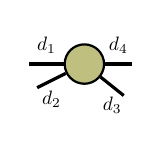
\begin{tikzpicture}[baseline=-0.5ex]
    \tikzset{tensor/.style = {minimum size = 0.5cm,shape = circle,thick,draw=black,inner sep = 0pt}, edge/.style = {thick,line width=.4mm},every loop/.style={}}
    \def\x{6}
    \def\y{0}   \node[tensor,fill=green!50!red!50!white] (T) at (\x+1,\y) {$\At$};
    \draw[edge] (T) -- (\x+0.3,0) node [midway,above] {\scalebox{0.7}{\dimcolor{$d_1$}}};
    \draw[edge] (T) -- (\x+1.6,0) node [midway,above] {\scalebox{0.7}{\dimcolor{$d_4$}}};;
    \draw[edge] (T) -- (\x+0.4,-0.3) node [midway, below] {\scalebox{0.7}{\dimcolor{$d_2$}}};
    \draw[edge] (T) -- (\x+1.5,-0.4)node [midway, below] {\scalebox{0.7}{\dimcolor{$d_3$}}};
\end{tikzpicture}\right)_{(\{1,2\})}
&=
\left(\begin{tikzpicture}[baseline=\baseline]
    \tikzset{tensor/.style = {minimum size = 0.5cm,shape = circle,thick,draw=black,inner sep = 0pt}, edge/.style   = {thick,line width=.4mm},every loop/.style={}}
    \def\y{0}
    \def\x{0}
  \node[tensor,fill=red!50!white] (A) at (\x,\y){\scalebox{0.85}{$\Ab_1$}};
  \node[tensor,fill=blue!50!white] (B) at (\x+1,\y){$\Ab_2$};
   \node[tensor,fill=red!20!white] (C) at (\x+2,\y){$\Ab_3$};
    \node[tensor,fill=blue!20!white] (D) at (\x+3,\y){$\Ab_4$};
    \draw  node[fill = black,circle,inner sep=0pt,minimum size=4pt] (m) at (\x+1.5,\y+0.7) {};
    \draw[edge] (A) -- (m)node [midway, above] {\scalebox{0.7}{\dimcolor{$R$}}} ;
    \draw[edge] (B) -- (m);
    \draw[edge] (C) -- (m);
    \draw[edge] (D) -- (m)node [midway, above] {\scalebox{0.7}{\dimcolor{$R$}}};
    \draw[edge](A) -- (\x,\y-0.7)node [midway,left] {\scalebox{0.7}{\dimcolor{$d_1$}}};
    \draw[edge](B) -- (\x+1,\y-0.7)node [midway,left] {\scalebox{0.7}{\dimcolor{$d_2$}}};
    \draw[edge](C) -- (\x+2,\y-0.7)node [midway,left] {\scalebox{0.7}{\dimcolor{$d_3$}}};
    \draw[edge](D) -- (\x+3,\y-0.7) node [midway,left] {\scalebox{0.7}{\dimcolor{$d_4$}}};
\end{tikzpicture}\right)_{(\{1,2\})}\\
&=
\begin{tikzpicture}[baseline=\baseline]
    \tikzset{tensor/.style = {minimum size = 0.5cm,shape = circle,thick,draw=black,inner sep = 0pt}, edge/.style   = {thick,line width=.4mm},every loop/.style={}}
    \def\y{0}
    \def\x{0}
  \node[tensor,fill=red!50!white] (A) at (\x,\y){\scalebox{0.85}{$\Ab_1$}};
  \node[tensor,fill=blue!50!white] (B) at (\x+1,\y){$\Ab_2$};
   \node[tensor,fill=red!20!white] (C) at (\x+2,\y){$\Ab_3$};
    \node[tensor,fill=blue!20!white] (D) at (\x+3,\y){$\Ab_4$};
    \draw  node[fill = black,circle,inner sep=0pt,minimum size=4pt] (m1) at (\x+0.5,\y+0.7) {};
    \draw  node[fill = black,circle,inner sep=0pt,minimum size=4pt] (m2) at (\x+2.5,\y+0.7) {};
    \draw[edge](A) -- (\x,\y-0.65) -- (\x+0.5,\y-0.65) -- (\x+0.5,\y-1);
    \draw[edge](B) -- (\x+1,\y-0.65) -- (\x+0.6,\y-0.65) -- (\x+0.6,\y-1);
    \draw[edge](C) -- (\x+2,\y-0.65) -- (\x+2.5,\y-0.65) -- (\x+2.5,\y-1);
    \draw[edge](D) -- (\x+3,\y-0.65) -- (\x+2.6,\y-0.65) -- (\x+2.6,\y-1);
    \node[draw=none] at (\x+0.55,\y-1.15){\scalebox{0.7}{\dimcolor{$d_1d_2$}}};
    \node[draw=none] at (\x+2.55,\y-1.15){\scalebox{0.7}{\dimcolor{$d_3d_4$}}};
    \draw[dotted] (\x+1.5,\y+1.5) -- (\x+1.5,\y-0.7);
    \draw[edge](A) -- (m1)node [midway,left] {\scalebox{0.7}{\dimcolor{$R$}}};;
    \draw[edge](B) -- (m1)node [midway,right] {\scalebox{0.7}{\dimcolor{$R$}}};
    \draw[edge](C) -- (m2)node [midway,left] {\scalebox{0.7}{\dimcolor{$R$}}};
    \draw[edge](D) -- (m2)node [midway,right] {\scalebox{0.7}{\dimcolor{$R$}}};
    \draw[edge](m1)--(m2)node [near start, above] {\scalebox{0.7}{\dimcolor{$R$}}};
\end{tikzpicture}.
\end{align*}
\item  The CP rank of a tensor $\At \in \RR^{d_1\times \cdots \times d_N}$ can easily be upper bounded as~\citep{kolda2009tensor}
$$\cprank(\At)\leq \min_{n\in [N]} \prod_{i\neq n} d_i.$$
\item For second-order tensors $\Ab\in\RR^{d_1\times d_2}$, the CP rank corresponds exactly to the classical notion of the rank of a matrix.
\item The CP decomposition $\At = \CP{\Ab,\Bb,\Cb}$ can be expressed using the Kronecker delta 
$$\At_{i,j,k} = \sum_{r_1,r_2,r_3}\delta_{r_1,r_2,r_3}\Ab_{i,r_1}\Bb_{j,r_2}\Cb_{k,r_3},$$
as well as with mode-$n$ products (see~\ref{par:mode-n-tensor-product}) 
$$\At = \It\ttm{1}\Ab\ttm{2}\Bb\ttm{3}\Cb$$
where $\It$ is the third-order copy tensor. 
\item The rank of the second-order tensors (matrices), over the fields $\RR$ and $\CC$ is the same. However, for higher-order tensors ($N$-th order tensors with $N\geq3$) the rank can vary depending on the decomposition field~\citep{kruskal1989rank}.
\item The number of parameters of a CP decomposition of an $N$-th order $d$-dimensional tensors ($d_1 = \dots = d_N = d$) is $NdR$ instead of $d^N$ for the full tensor. If $R$ is small, the number of parameters can be significantly reduced. 
\end{enumerate}
\end{remark}
The following proposition shows how the mode-$n$ matricization of the CP decomposition of a tensor can be expressed using the Khatri-Rao product.
\begin{proposition}
Let $\At\in\RR^{d_1\times d_2\times\dots\times d_N}$. If $\At=\CP{\Ab_1,\Ab_2,\dots,\Ab_N}$, then 
$$\At_{(n)}=\Ab_n\left(\Ab_1\krao\dots\krao\Ab_{(n-1)}\krao\Ab_{(n+1)}\krao\dots\krao\Ab_N\right)^\ts.$$
\begin{proof}
For $N=3$ and $n=1$,
\begin{align*}
\At_{(1)}
&=
\left(\begin{tikzpicture}[baseline=\baseline]
    \tikzset{tensor/.style = {minimum size = 0.5cm,shape = circle,thick,draw=black,inner sep = 0pt}, edge/.style  = {thick,line width=.4mm},every loop/.style={}}
    \def\y{0}
    \def\x{0}
    \node[tensor,fill=green!50!red!50!white] (At) at (\x,\y){\scalebox{0.85}{$\At$}};
    \draw[edge] (\x+0.25,\y) -- (\x+0.6,\y)  node [midway,above] {\scalebox{0.7}{\dimcolor{$d_2$}}};
    \draw[edge] (\x-0.25,\y) -- (\x-0.6,\y)  node [midway,above] {\scalebox{0.7}{\dimcolor{$d_1$}}};
    \draw[edge] (\x,\y-0.25) -- (\x,\y-0.7)  node [midway,left] {\scalebox{0.7}{\dimcolor{$d_3$}}};
    \end{tikzpicture}\right)_{(1)}
=
\left(\begin{tikzpicture}[baseline=\baseline]
    \tikzset{tensor/.style = {minimum size = 0.5cm,shape = circle,thick,draw=black,inner sep = 0pt}, edge/.style   = {thick,line width=.4mm},every loop/.style={}}
    \def\y{0}
    \def\x{0}
  \node[tensor,fill=red!50!white] (A1) at (\x,\y){\scalebox{0.85}{$\Ab_1$}};
  \node[tensor,fill=blue!50!white] (A2) at (\x+1,\y){$\Ab_2$};
   \node[tensor,fill=blue!20!white] (A3) at (\x+2,\y){$\Ab_3$};
    \draw  node[fill = black,circle,inner sep=0pt,minimum size=4pt] (m) at (\x+1,\y+1) {};
    \draw[edge] (A1) -- (m) node [midway,left] {\scalebox{0.7}{\dimcolor{$R$}}};
    \draw[edge] (A2) -- (m)node [midway,left=-0.05cm] {\scalebox{0.7}{\dimcolor{$R$}}};
    \draw[edge] (A3) -- (m)node [midway,right] {\scalebox{0.7}{\dimcolor{$R$}}};
    \draw[edge](A1) -- (\x,\y-0.7)node [midway,left] {\edgelabel{$d_1$}};
    \draw[edge](A2) -- (\x+1,\y-0.7)node [midway,left] {\edgelabel{$d_2$}};
    \draw[edge](A3) -- (\x+2,\y-0.7)node [midway,left] {\edgelabel{$d_3$}};
\end{tikzpicture}\right)_{(1)}\\
&=
\begin{tikzpicture}[baseline=\baseline]
    \tikzset{tensor/.style = {minimum size = 0.5cm,shape = circle,thick,draw=black,inner sep = 0pt}, edge/.style   = {thick,line width=.4mm},every loop/.style={}}
    \def\y{0}
    \def\x{0}
    \node[tensor,fill=green!50!red!50!white] (At) at (\x,\y){\scalebox{0.85}{$\At$}};
    \draw[edge] (\x-0.25,\y) -- (\x-0.6,\y)  node [midway,above] {\scalebox{0.7}{\dimcolor{$d_1$}}};
    \draw[edge] (\x+0.2,\y+0.15) -- (\x+0.5,\y+0.15)-- (\x+0.5,\y+0.05) -- (\x+1,\y+0.05) node [midway,above]
    {\scalebox{0.7}{\dimcolor{$d_2$}}};
    \draw[edge] (\x+0.2,\y-0.15) -- (\x+0.5,\y-0.15)-- (\x+0.5,\y-0.05)-- (\x+1,\y-0.05) node [midway,below]
    {\scalebox{0.7}{\dimcolor{$d_3$}}};
    \end{tikzpicture}
=
\begin{tikzpicture}[baseline=\baseline]
    \tikzset{tensor/.style = {minimum size = 0.5cm,shape = circle,thick,draw=black,inner sep = 0pt}, edge/.style   = {thick,line width=.4mm},every loop/.style={}}
    \def\y{0}
    \def\x{0}
    \node[tensor,fill=red!50!white] (A1) at (\x,\y){\scalebox{0.85}{$\Ab_1$}};
    \node[tensor,fill=blue!50!white] (A2) at (\x+1.7,\y+0.7){$\Ab_2$};
    \node[tensor,fill=blue!20!white] (A3) at (\x+1.7,\y-0.7){$\Ab_3$};
    \draw  node[fill = black,circle,inner sep=0pt,minimum size=4pt] (m) at (\x+1,\y) {};
    \draw[edge] (A1) -- (m) node [very near end,above] {\scalebox{0.7}{\dimcolor{$R$}}};
    \draw[edge] (A2) -- (m);
    \draw[edge] (A3) -- (m);
    \draw[edge] (A1) -- (\x-0.7,\y) node [midway,above] {\scalebox{0.7}{\dimcolor{$d_1$}}};
    \draw[edge] (A2) -- (\x+2.5,\y+0.7) -- (\x+2.5,\y+0.05)-- (\x+3,\y+0.05) node [midway,above]
    {\scalebox{0.7}{\dimcolor{$d_2$}}};
    \draw[edge] (A3) -- (\x+2.5,\y-0.7) -- (\x+2.5,\y-0.05) -- (\x+3,\y-0.05) node [midway,below]
    {\scalebox{0.7}{\dimcolor{$d_3$}}};
    \end{tikzpicture}
=
\Ab_1(\Ab_2\krao\Ab_3)^\ts.
\end{align*}
\end{proof}
\end{proposition}


\subsection{Tucker Decomposition}
The Tucker decomposition \cite{tucker1966some} factorizes a $N$-th order tensor
into smaller tensor and factor matrices. In this decomposition, the smaller
tensor is called the \emph{core tensor}. The Tucker
decomposition consists of $N$ mode-$n$ products (see, e.g., Section~\ref{sec:product})
between the core tensor and the factor matrices.

Let $\Tt \in \RR^{d_1 \times \dots \times d_N}$. A Tucker decomposition of $\Tt$
is given by
\[
    \Tt
    = \Gt \times_1 \Ub_1 \times_2 \Ub_2\times_3 \dots \times_N \Ub_N,
\]
where $\Gt \in \RR^{R_1 \times \dots \times R_N}$ is the core tensor and
$\Ub_i \in \RR^{d_i \times R_i}$ for $i \in [N]$ are the factor matrices.
The $N$-tuple $(R_1,\dots,R_N)$ is called the \emph{rank} of Tucker
decomposition.

The Tucker decomposition of a fourth-order tensor $\Tt\in\RR^{d_1\times\cdots \times d_4}$ can be illustrated using tensor networks notation as follows.
$$
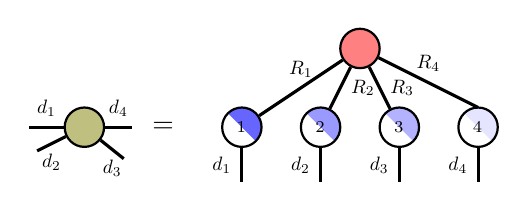
\begin{tikzpicture}[baseline=-0.5ex]
    \tikzset{tensor/.style = {minimum size = 0.5cm,shape = circle,thick,draw=black,inner sep = 0pt}, edge/.style = {thick,line width=.4mm},every loop/.style={}}
    \def\x{6}
    \def\y{0}   \node[tensor,fill=green!50!red!50!white] (T) at (\x+1,\y) {$\Tt$};
    \draw[edge] (T) -- (\x+0.3,0) node [midway,above] {\scalebox{0.7}{\dimcolor{$d_1$}}};
    \draw[edge] (T) -- (\x+1.6,0) node [midway,above] {\scalebox{0.7}{\dimcolor{$d_4$}}};;
    \draw[edge] (T) -- (\x+0.4,-0.3) node [midway, below] {\scalebox{0.7}{\dimcolor{$d_2$}}};
    \draw[edge] (T) -- (\x+1.5,-0.4)node [midway, below] {\scalebox{0.7}{\dimcolor{$d_3$}}};
    \node[draw = none] at (\x+2,0){$=$};
\node[tensor,fill=red!50!white] (G) at (\x+4.5,\y+1) {$\Gt$};
    \node[tensor, path picture={
    \fill[fill=blue!60!white](path picture bounding box.south east)
    -- 
    (path picture bounding box.north west) --
    (path picture bounding box.north east) -- cycle;
    }, shift={(\x+3,\y)}] (U_1) {\scalebox{0.85}{$\Ub_1$}};
    \node[tensor, path picture={
    \fill[fill=blue!40!white](path picture bounding box.south east)
    -- 
    (path picture bounding box.north west) --
    (path picture bounding box.north east) -- cycle;
    }, shift={(\x+4,\y)}] (U_2) {\scalebox{0.85}{$\Ub_2$}};
    \node[tensor, path picture={
    \fill[fill=blue!30!white](path picture bounding box.south east)
    -- 
    (path picture bounding box.north west) --
    (path picture bounding box.north east) -- cycle;
    }, shift={(\x+5,\y)}] (U_3) {\scalebox{0.85}{$\Ub_3$}};
    \node[tensor, path picture={
    \fill[fill=blue!10!white](path picture bounding box.south east)
    -- 
    (path picture bounding box.north west) --
    (path picture bounding box.north east) -- cycle;
    }, shift={(\x+6,\y)}] (U_4) {\scalebox{0.85}{$\Ub_4$}};
    \draw[edge] (G) -- (U_1) node [midway, above] {\scalebox{0.7}{\dimcolor{$R_1$}}};
    \draw[edge] (G) -- (U_2) node [midway, right] {\scalebox{0.7}{\dimcolor{$R_2$}}};
    \draw[edge] (G) -- (U_3) node [midway, right] {\scalebox{0.7}{\dimcolor{$R_3$}}};
    \draw[edge] (G) -- (\x+6,\y+0.25) node [midway, above] {\scalebox{0.7}{\dimcolor{$R_4$}}};
    \draw[edge] (U_1) -- (\x+3,\y-0.7) node [midway, left] {\scalebox{0.7}{\dimcolor{$d_1$}}};
    \draw[edge] (U_2) -- (\x+4,\y-0.7) node [midway, left] {\scalebox{0.7}{\dimcolor{$d_2$}}};
    \draw[edge] (U_3) -- (\x+5,\y-0.7) node [midway, left] {\scalebox{0.7}{\dimcolor{$d_3$}}};
    \draw[edge] (U_4) -- (\x+6,\y-0.7) node [midway, left] {\scalebox{0.7}{\dimcolor{$d_4$}}};
\end{tikzpicture}.
$$


It is not difficult to show that the factor matrices
$\Ub_i \in \RR^{d_i \times R_i}$ can always be chosen to be unitary (see
item~\ref{item:Tucker_orth} in Remark~\ref{rem:tuckers} below).


\paragraph{Multi-linear rank} The \emph{multi-linear (or Tucker) rank}\footnote{Note the distinction between the rank $(R_1,\dots,R_n)$ of a Tucker \emph{decomposition},
given by the size of the core tensor $\Gt$ appearing in
$\Tt = \Gt \times_1 \Ub_1 \times_2 \dots \times_N \Ub_N$, and the
(Tucker) multi-linear rank of a tensor $\Tt$, which is defined as the
minimal such tuple.} of a tensor $\Tt$ is the smallest tuple $(R_1,\dots,R_N)$
for which there exists a rank-$(R_1,\dots,R_N)$ decomposition of $\Tt$. Since there is only 
a partial order on tuples of integers, one may ask whether this notion of rank is well defined. 
The following proposition shows that it is. 

\begin{proposition}
Let $\Tt = \Gt \times_1 \Ub_1 \times_2 \Ub_2\times_3\dots \times_N \Ub_N$ and 
$\Tt = \tilde\Gt \times_1 \tilde\Ub_1 \times_2 \tilde\Ub_2\times_3 \dots \times_N \tilde\Ub_N$ be two 
Tucker decompositions of the same tensor $\Tt$ of rank-$(R_1,R_2,\dots, R_n)$ and 
$(\tilde R_1,\tilde R_2,\dots,\tilde R_n)$, respectively. Then $\Tt$ admits a Tucker decomposition of rank-$(\min(R_1,\tilde R_1), \min(R_2,\tilde R_2), \dots, \min(R_N,\tilde R_N))$. 
\end{proposition}
\begin{proof}
Suppose $N=3$. Applying the mode-$1$ unfolding and Theorem~\ref{thm: matricization-rank} to each of the two Tucker decompositions of $\Tt$ we obtain the following:
\begin{align*}
    \rank\left(\begin{tikzpicture}[baseline=\baseline]
    \tikzset{tensor/.style = {minimum size = 0.5cm,shape = circle,thick,draw=black,inner sep = 0pt}, edge/.style  = {thick,line width=.4mm},every loop/.style={}}
    \def\y{0}
    \def\x{0}
    \node[tensor,fill=green!50!red!50!white] (Tt) at (\x,\y){\scalebox{0.85}{$\Tt$}};
    \draw[edge] (\x+0.25,\y) -- (\x+0.6,\y)  node [midway,above] {\scalebox{0.7}{\dimcolor{$d_2$}}};
    \draw[edge] (\x-0.25,\y) -- (\x-0.6,\y)  node [midway,above] {\scalebox{0.7}{\dimcolor{$d_1$}}};
    \draw[edge] (\x,\y-0.25) -- (\x,\y-0.7)  node [midway,left] {\scalebox{0.7}{\dimcolor{$d_3$}}};
    \end{tikzpicture}\right)_{(1)}
=
\rank(\begin{tikzpicture}[baseline=\baseline]
    \tikzset{tensor/.style = {minimum size = 0.5cm,shape = circle,thick,draw=black,inner sep = 0pt}, edge/.style  = {thick,line width=.4mm},every loop/.style={}}
    \def\y{0}
    \def\x{0}
    \node[tensor,fill=green!50!red!50!white] (Tt) at (\x,\y){\scalebox{0.85}{$\Tt$}};
    \draw[edge] (Tt) -- (\x-0.6,\y)  node [midway,above] {\scalebox{0.7}{\dimcolor{$d_1$}}};
    \draw[edge] (Tt) -- (\x+0.6,\y)  node [midway,above] {\scalebox{0.7}{\dimcolor{$d_2$}}};    \draw[edge] (Tt) -- (\x+0.6,\y)  node [midway,above] {\scalebox{0.7}{\dimcolor{$d_2$}}};
    \draw[edge] (\x+0.25,\y-0.1) -- (\x+0.6,\y-0.1)  node [midway,below] {\scalebox{0.7}{\dimcolor{$d_3$}}};
\end{tikzpicture})
=
\rank\left(\begin{tikzpicture}[baseline=\baseline]
    \tikzset{tensor/.style = {minimum size = 0.5cm,shape = circle,thick,draw=black,inner sep = 0pt}, edge/.style   = {thick,line width=.4mm},every loop/.style={}}
    \def\y{0}
    \def\x{0}
    \node[tensor,fill=blue!60!white] (U_1) at (\x,\y){\scalebox{0.85}{$\Ub_1$}};
    \node[tensor,fill=blue!30!white] (U_2) at (\x+2.7,\y+0.7){$\Ub_2$};
    \node[tensor,fill=blue!10!white] (U_3) at (\x+2.7,\y-0.7){$\Ub_3$};
    \node[tensor,fill=red!60!white] (m) at (\x+1,\y) {$\Gt$}; 
     \draw[edge] (\x+1.2,\y+0.15) -- (\x+1.5,\y+0.15)-- (\x+1.5,\y+0.05) -- (\x+2,\y+0.05) node [midway,above]
    {\scalebox{0.7}{\dimcolor{$R_2$}}};
    \draw[edge] (\x+1.2,\y-0.15) -- (\x+1.5,\y-0.15)-- (\x+1.5,\y-0.05)-- (\x+2,\y-0.05) node [midway,below]
    {\scalebox{0.7}{\dimcolor{$R_3$}}};
    \draw[edge] (U_1) -- (m) node [midway,above] {\scalebox{0.7}{\dimcolor{$R_1$}}};
    \draw[edge] (U_1) -- (\x-0.7,\y) node [midway,above] {\scalebox{0.7}{\dimcolor{$d_1$}}};
    \draw[edge](\x+2,\y-0.05) -- (\x+2,\y-0.7) -- (U_3);
    \draw[edge](\x+2,\y+0.05) -- (\x+2,\y+0.7) -- (U_2);
    \draw[edge] (U_2) -- (\x+3.5,\y+0.7) -- (\x+3.5,\y+0.05)-- (\x+4,\y+0.05) node [midway,above]
    {\scalebox{0.7}{\dimcolor{$d_2$}}};
    \draw[edge] (U_3) -- (\x+3.5,\y-0.7) -- (\x+3.5,\y-0.05) -- (\x+4,\y-0.05) node [midway,below]
    {\scalebox{0.7}{\dimcolor{$d_3$}}};
    \draw[dotted] (\x+0.45,\y+1) -- (\x+0.45,\y-1);
    \end{tikzpicture}\right)\leq R_1,
\end{align*}
and at the same time
\begin{align*}
    \rank\left(\begin{tikzpicture}[baseline=\baseline]
    \tikzset{tensor/.style = {minimum size = 0.5cm,shape = circle,thick,draw=black,inner sep = 0pt}, edge/.style  = {thick,line width=.4mm},every loop/.style={}}
    \def\y{0}
    \def\x{0}
    \node[tensor,fill=green!50!red!50!white] (Tt) at (\x,\y){\scalebox{0.85}{$\Tt$}};
    \draw[edge] (\x+0.25,\y) -- (\x+0.6,\y)  node [midway,above] {\scalebox{0.7}{\dimcolor{$d_2$}}};
    \draw[edge] (\x-0.25,\y) -- (\x-0.6,\y)  node [midway,above] {\scalebox{0.7}{\dimcolor{$d_1$}}};
    \draw[edge] (\x,\y-0.25) -- (\x,\y-0.7)  node [midway,left] {\scalebox{0.7}{\dimcolor{$d_3$}}};
    \end{tikzpicture}\right)_{(1)}
=
\rank(\begin{tikzpicture}[baseline=\baseline]
    \tikzset{tensor/.style = {minimum size = 0.5cm,shape = circle,thick,draw=black,inner sep = 0pt}, edge/.style  = {thick,line width=.4mm},every loop/.style={}}
    \def\y{0}
    \def\x{0}
    \node[tensor,fill=green!50!red!50!white] (Tt) at (\x,\y){\scalebox{0.85}{$\Tt$}};
    \draw[edge] (Tt) -- (\x-0.6,\y)  node [midway,above] {\scalebox{0.7}{\dimcolor{$d_1$}}};
    \draw[edge] (Tt) -- (\x+0.6,\y)  node [midway,above] {\scalebox{0.7}{\dimcolor{$d_2$}}};    \draw[edge] (Tt) -- (\x+0.6,\y)  node [midway,above] {\scalebox{0.7}{\dimcolor{$d_2$}}};
    \draw[edge] (\x+0.25,\y-0.1) -- (\x+0.6,\y-0.1)  node [midway,below] {\scalebox{0.7}{\dimcolor{$d_3$}}};
\end{tikzpicture})
=
\rank\left(\begin{tikzpicture}[baseline=\baseline]
    \tikzset{tensor/.style = {minimum size = 0.5cm,shape = circle,thick,draw=black,inner sep = 0pt}, edge/.style   = {thick,line width=.4mm},every loop/.style={}}
    \def\y{0}
    \def\x{0}
    \node[tensor,fill=red!60!blue!20!white] (U_1) at (\x,\y){\scalebox{0.85}{$\tilde{\Ub}_1$}};
    \node[tensor,fill=red!30!blue!50!white] (U_2) at (\x+2.7,\y+0.7){$\tilde{\Ub}_2$};
    \node[tensor,fill=red!20!blue!40!white] (U_3) at (\x+2.7,\y-0.7){$\tilde{\Ub}_3$};
    \node[tensor,fill=red!40!white] (m) at (\x+1,\y) {$\tilde{\Gt}$}; 
     \draw[edge] (\x+1.2,\y+0.15) -- (\x+1.5,\y+0.15)-- (\x+1.5,\y+0.05) -- (\x+2,\y+0.05) node [midway,above]
    {\scalebox{0.7}{\dimcolor{$\tilde{R}_2$}}};
    \draw[edge] (\x+1.2,\y-0.15) -- (\x+1.5,\y-0.15)-- (\x+1.5,\y-0.05)-- (\x+2,\y-0.05) node [midway,below]
    {\scalebox{0.7}{\dimcolor{$\tilde{R}_3$}}};
    \draw[edge] (U_1) -- (m) node [midway,above] {\scalebox{0.7}{\dimcolor{$\tilde{R_1}$}}};
    \draw[edge] (U_1) -- (\x-0.7,\y) node [midway,above] {\scalebox{0.7}{\dimcolor{$d_1$}}};
    \draw[edge](\x+2,\y-0.05) -- (\x+2,\y-0.7) -- (U_3);
    \draw[edge](\x+2,\y+0.05) -- (\x+2,\y+0.7) -- (U_2);
    \draw[edge] (U_2) -- (\x+3.5,\y+0.7) -- (\x+3.5,\y+0.05)-- (\x+4,\y+0.05) node [midway,above]
    {\scalebox{0.7}{\dimcolor{$d_2$}}};
    \draw[edge] (U_3) -- (\x+3.5,\y-0.7) -- (\x+3.5,\y-0.05) -- (\x+4,\y-0.05) node [midway,below]
    {\scalebox{0.7}{\dimcolor{$d_3$}}};
    \draw[dotted] (\x+0.45,\y+1) -- (\x+0.45,\y-1);
    \end{tikzpicture}\right)\leq \tilde{R}_1,
\end{align*}
Therefore, $\rank\left(\begin{tikzpicture}[baseline=\baseline]
    \tikzset{tensor/.style = {minimum size = 0.5cm,shape = circle,thick,draw=black,inner sep = 0pt}, edge/.style  = {thick,line width=.4mm},every loop/.style={}}
    \def\y{0}
    \def\x{0}
    \node[tensor,fill=green!50!red!50!white] (Tt) at (\x,\y){\scalebox{0.85}{$\Tt$}};
    \draw[edge] (\x+0.25,\y) -- (\x+0.6,\y)  node [midway,above] {\scalebox{0.7}{\dimcolor{$d_2$}}};
    \draw[edge] (\x-0.25,\y) -- (\x-0.6,\y)  node [midway,above] {\scalebox{0.7}{\dimcolor{$d_1$}}};
    \draw[edge] (\x,\y-0.25) -- (\x,\y-0.7)  node [midway,left] {\scalebox{0.7}{\dimcolor{$d_3$}}};
\end{tikzpicture}\right)_{(1)}\leq\min(R_1,\tilde{R}_1)$. 
Applying the same reasoning for $n=2,3$ we conclude that $\Tt$ admits a Tucker decomposition of rank-$(\min(R_1,\tilde{R}_1),\min(R_2,\tilde{R}_2),\min(R_3,\tilde{R}_3))$.
\end{proof}

\paragraph{Computing The Tucker Decomposition.} In contrast with the CP decomposition, which is NP-hard to compute, finding an exact Tucker decomposition (and in particular the one with minimal multi-linear rank) can be achieved in polynomial time by successive SVDs. 

The basic idea of the Tucker decomposition algorithm is to find the $R_n$ leading left singular vectors
in mode-$n$, independently of the other modes. This algorithm, known as \textit{Higher-Order SVD (HOSVD)}~\citep{de2000multilinear}, is depicted below.  For simplicity, we illustrate this process for $N=4$:
\begin{align*}
    &\begin{tikzpicture}[baseline=\baseline]
    \tikzset{tensor/.style = {minimum size = 0.5cm,shape = circle,thick,draw=black,inner sep = 0pt}, edge/.style = {thick,line width=.4mm},every loop/.style={}}
    \def\x{0}
    \def\y{0}
    \node[tensor,fill=green!50!red!50!white] (A) at (\x-5.5,\y){\scalebox{0.85}{$\Tt$}};
    \draw[edge] (A) -- (\x-5.5,\y+0.75) node [midway,left]
    {\scalebox{0.7}{\dimcolor{$d_1$}}};
    \draw[edge] (A) -- (\x-5.5,\y-0.75) node [midway,left]
    {\scalebox{0.7}{\dimcolor{$d_3$}}};
    \draw[edge] (\x-5.75,\y+0.05) -- (\x-6.2,\y-0.3) node [midway,above]
    {\scalebox{0.7}{\dimcolor{$d_2$}}};
    \draw[edge] (\x-5.25,\y+0.05) -- (\x-4.7,\y-0.3) node [midway,above]
    {\scalebox{0.7}{\dimcolor{$d_4$}}};
    \node[draw=none] at (\x-3,\y){$\underrightarrow{\text{mode-1 matricization}}$};
    \node[tensor,fill=green!50!red!50!white] (A) at (\x-0.5,\y){\scalebox{0.85}{$\Tb$}};
    \draw[edge] (\x-0.35,\y+0.2) -- (\x,\y+0.2) --(\x,\y+0.1) -- (\x
    +0.35,\y+0.1) node [midway,above]
    {\scalebox{0.7}{\dimcolor{$d_2$}}};
    \draw[edge] (\x-0.35,\y-0.2) -- (\x,\y-0.2) -- (\x,\y-0.1) -- (\x+0.35,\y-0.1) node [midway,below]
    {\scalebox{0.7}{\dimcolor{$d_4$}}};
     \draw[edge] (A) -- (\x+0.35,\y)node [right]
    {\scalebox{0.7}{\dimcolor{$d_3$}}};
     \draw[edge] (A) -- (\x-1.25,\y) node [midway,above]
    {\scalebox{0.7}{\dimcolor{$d_1$}}};
    \node[draw=none] at (\x+1,\y){$\rightarrow$};
    \node[tensor, path picture={
    \fill[fill=blue!50!white](path picture bounding box.south east)
        -- 
    (path picture bounding box.north west) --
    (path picture bounding box.north east) -- cycle;
    }, shift={(\x+1.5,\y)}] (U_1) {\scalebox{0.8}{$\Ub_1$}};
    \node[tensor,fill=red!50!white] (Sigma_1) at (\x+2.5,\y){\scalebox{0.85}{$\Sigmab_1$}};
    \node[tensor, path picture={
    \fill[fill=red!60!white](path picture bounding box.south west)
        -- 
    (path picture bounding box.north east) --
    (path picture bounding box.north west) -- cycle;
    }, shift={(\x+3.5,\y)}] (V_1) {\scalebox{0.8}{$\Vb_1$}};
    \draw[edge](V_1) -- (\x+4.5,\y) node [right]{\scalebox{0.7}{\textcolor{gray}{$d_3$}}};
    \draw[edge] (U_1) -- (Sigma_1)node [midway,above]
    {\scalebox{0.7}{\dimcolor{$R_1$}}};
    \draw[edge] (U_1) -- (\x+1.5,\y-0.7)node [midway,left]
    {\scalebox{0.7}{\dimcolor{$d_1$}}};
    \draw[edge] (Sigma_1) -- (V_1) node[midway,above]    {\scalebox{0.7}{\dimcolor{$R_1$}}};
    \draw[edge] (\x+3.7,\y+0.15) -- (\x+4,\y+0.15) --(\x+4,\y+0.1) -- (\x+4.5,\y+0.1) node [midway,above]
    {\scalebox{0.7}{\dimcolor{$d_2$}}};
    \draw[edge] (\x+3.65,\y-0.2) -- (\x+4,\y-0.2) -- (\x+4,\y-0.1) -- (\x+4.5,\y-0.1) node [midway,below]
    {\scalebox{0.7}{\dimcolor{$d_4$}}};
    \node[draw=none] at (\x+5.75,\y){\text{Keep $\Ub_1$}.};
\end{tikzpicture}\\
&\begin{tikzpicture}[baseline=\baseline]
    \tikzset{tensor/.style = {minimum size = 0.5cm,shape = circle,thick,draw=black,inner sep = 0pt}, edge/.style = {thick,line width=.4mm},every loop/.style={}}
    \def\y{0}
    \def\x{0}
    \node[tensor,fill=green!50!red!50!white] (A) at (\x-2.5,\y){\scalebox{0.85}{$\Tt$}};
    \draw[edge] (A) -- (\x-2.5,\y+0.75) node [midway,left]
    {\scalebox{0.7}{\dimcolor{$d_1$}}};
    \draw[edge] (A) -- (\x-2.5,\y-0.75) node [midway,left]
    {\scalebox{0.7}{\dimcolor{$d_3$}}};
    \draw[edge] (\x-2.75,\y+0.05) -- (\x-3.2,\y-0.3) node [midway,above]
    {\scalebox{0.7}{\dimcolor{$d_2$}}};
    \draw[edge] (\x-2.25,\y+0.05) -- (\x-1.7,\y-0.3) node [midway,above]
    {\scalebox{0.7}{\dimcolor{$d_4$}}};
    \node[draw=none] at (\x,\y){$\underrightarrow{\text{mode-2 matricization}}$};
    \node[tensor,fill=green!50!red!50!white] (A) at (\x+2.5,\y){\scalebox{0.85}{$\Tb$}};
    \draw[edge] (A) -- (\x+1.75,\y) node [midway,above]
    {\scalebox{0.7}{\dimcolor{$d_2$}}};
    \draw[edge] (A) -- (\x+3.35,\y)node [right]
    {\scalebox{0.7}{\dimcolor{$d_3$}}};
    \draw[edge] (\x+2.65,\y+0.2) -- (\x+3,\y+0.2) -- (\x+3,\y+0.1) -- (\x+3.35,\y+0.1)node [midway,above]
    {\scalebox{0.7}{\dimcolor{$d_1$}}};
    \draw[edge] (\x+2.65,\y-0.2) -- (\x+3,\y-0.2) -- (\x+3,\y-0.1) -- (\x+3.35,\y-0.1)node [midway,below]
    {\scalebox{0.7}{\dimcolor{$d_4$}}};
    \node[draw=none] at (\x+4,\y){$\rightarrow$};
    \node[tensor, path picture={
    \fill[fill=blue!40!white](path picture bounding box.south east)
        -- 
    (path picture bounding box.north west) --
    (path picture bounding box.north east) -- cycle;
    }, shift={(\x+4.5,\y)}] (U_2) {\scalebox{0.8}{$\Ub_2$}};
    \node[tensor,fill=red!40!white] (Sigma_2) at (\x+5.5,\y){\scalebox{0.85}{$\Sigmab_2$}};
    \node[tensor, path picture={
    \fill[fill=red!50!white](path picture bounding box.south west)
        -- 
    (path picture bounding box.north east) --
    (path picture bounding box.north west) -- cycle;
    }, shift={(\x+6.5,\y)}] (V_2) {\scalebox{0.8}{$\Vb_2$}};
    \draw[edge](V_2) -- (\x+7.5,\y) node [right]{\scalebox{0.7}{\dimcolor{$d_3$}}};
    \draw[edge] (U_2) -- (Sigma_2)node [midway,above]
    {\scalebox{0.7}{\dimcolor{$R_2$}}};
    \draw[edge] (U_2) -- (\x+4.5,\y-0.7)node [midway,left]
    {\scalebox{0.7}{\dimcolor{$d_2$}}};
    \draw[edge] (Sigma_2) -- (V_2) node[midway,above] {\scalebox{0.7}{\dimcolor{$R_2$}}};
    \draw[edge] (\x+6.71,\y+0.15) -- (\x+7,\y+0.15) --(\x+7,\y+0.1) -- (\x+7.5,\y+0.1) node [midway,above]
    {\scalebox{0.7}{\dimcolor{$d_1$}}};
    \draw[edge] (\x+6.65,\y-0.2) -- (\x+7,\y-0.2) -- (\x+7,\y-0.1) -- (\x+7.5,\y-0.1) node [midway,below]
    {\scalebox{0.7}{\dimcolor{$d_4$}}};
    \node[draw=none] at (\x+8.75,\y){\text{Keep $\Ub_2$}.};
\end{tikzpicture}\\
&\begin{tikzpicture}[baseline=\baseline]
    \tikzset{tensor/.style = {minimum size = 0.5cm,shape = circle,thick,draw=black,inner sep = 0pt}, edge/.style = {thick,line width=.4mm},every loop/.style={}}
    \def\y{0}
    \def\x{0}
    \node[tensor,fill=green!50!red!50!white] (A) at (\x-2.5,\y){\scalebox{0.85}{$\Tt$}};
    \draw[edge] (A) -- (\x-2.5,\y+0.75) node [midway,left]
    {\scalebox{0.7}{\dimcolor{$d_1$}}};
    \draw[edge] (A) -- (\x-2.5,\y-0.75) node [midway,left]
    {\scalebox{0.7}{\dimcolor{$d_3$}}};
    \draw[edge] (\x-2.75,\y+0.05) -- (\x-3.2,\y-0.3) node [midway,above]
    {\scalebox{0.7}{\dimcolor{$d_2$}}};
    \draw[edge] (\x-2.25,\y+0.05) -- (\x-1.7,\y-0.3) node [midway,above]
    {\scalebox{0.7}{\dimcolor{$d_4$}}};
    \node[draw=none] at (\x,\y){$\underrightarrow{\text{mode-3 matricization}}$};
    \node[tensor,fill=green!50!red!50!white] (A) at (\x+2.5,\y){\scalebox{0.85}{$\Tb$}};
    \draw[edge] (A) -- (\x+1.75,\y) node [midway,above]
    {\scalebox{0.7}{\dimcolor{$d_3$}}};
    \draw[edge] (A) -- (\x+3.35,\y)node [right]
    {\scalebox{0.7}{\dimcolor{$d_2$}}};
    \draw[edge] (\x+2.65,\y+0.2) -- (\x+3,\y+0.2) -- (\x+3,\y+0.1) -- (\x+3.35,\y+0.1)node [midway,above]
    {\scalebox{0.7}{\dimcolor{$d_1$}}};
    \draw[edge] (\x+2.65,\y-0.2) -- (\x+3,\y-0.2) -- (\x+3,\y-0.1) -- (\x+3.35,\y-0.1)node [midway,below]
    {\scalebox{0.7}{\dimcolor{$d_4$}}};
    \node[draw=none] at (\x+4,\y){$\rightarrow$};
    \node[tensor, path picture={
    \fill[fill=blue!30!white](path picture bounding box.south east)
        -- 
    (path picture bounding box.north west) --
    (path picture bounding box.north east) -- cycle;
    }, shift={(\x+4.5,\y)}] (U_3) {\scalebox{0.8}{$\Ub_3$}};
    \node[tensor,fill=red!30!white] (Sigma_3) at (\x+5.5,\y){\scalebox{0.85}{$\Sigmab_3$}};
    \node[tensor, path picture={
    \fill[fill=red!40!white](path picture bounding box.south west)
        -- 
    (path picture bounding box.north east) --
    (path picture bounding box.north west) -- cycle;
    }, shift={(\x+6.5,\y)}] (V_3) {\scalebox{0.8}{$\Vb_3$}};
    \draw[edge](V_3) -- (\x+7.5,\y) node [right]{\scalebox{0.7}{\dimcolor{$d_2$}}};
    \draw[edge] (U_3) -- (Sigma_3)node [midway,above]
    {\scalebox{0.7}{\dimcolor{$R_3$}}};
    \draw[edge] (U_3) -- (\x+4.5,\y-0.7)node [midway,left]
    {\scalebox{0.7}{\dimcolor{$d_3$}}};
    \draw[edge] (Sigma_3) -- (V_3) node[midway,above] {\scalebox{0.7}{\dimcolor{$R_3$}}};
    \draw[edge] (\x+6.71,\y+0.15) -- (\x+7,\y+0.15) --(\x+7,\y+0.1) -- (\x+7.5,\y+0.1) node [midway,above]
    {\scalebox{0.7}{\dimcolor{$d_1$}}};
    \draw[edge] (\x+6.65,\y-0.2) -- (\x+7,\y-0.2) -- (\x+7,\y-0.1) -- (\x+7.5,\y-0.1) node [midway,below]
    {\scalebox{0.7}{\dimcolor{$d_4$}}};
    \node[draw=none] at (\x+8.75,\y){\text{Keep $\Ub_3$.}};
\end{tikzpicture}\\
&\begin{tikzpicture}[baseline=\baseline]
    \tikzset{tensor/.style = {minimum size = 0.5cm,shape = circle,thick,draw=black,inner sep = 0pt}, edge/.style = {thick,line width=.4mm},every loop/.style={}}
    \def\y{0}
    \def\x{0}
    \node[tensor,fill=green!50!red!50!white] (A) at (\x-2.5,\y){\scalebox{0.85}{$\Tt$}};
    \draw[edge] (A) -- (\x-2.5,\y+0.75) node [midway,left]
    {\scalebox{0.7}{\dimcolor{$d_1$}}};
    \draw[edge] (A) -- (\x-2.5,\y-0.75) node [midway,left]
    {\scalebox{0.7}{\dimcolor{$d_3$}}};
    \draw[edge] (\x-2.75,\y+0.05) -- (\x-3.2,\y-0.3) node [midway,above]
    {\scalebox{0.7}{\dimcolor{$d_2$}}};
    \draw[edge] (\x-2.25,\y+0.05) -- (\x-1.7,\y-0.3) node [midway,above]
    {\scalebox{0.7}{\dimcolor{$d_4$}}};
    \node[draw=none] at (\x,\y){$\underrightarrow{\text{mode-4 matricization}}$};
    \node[tensor,fill=green!50!red!50!white] (A) at (\x+2.5,\y){\scalebox{0.85}{$\Tb$}};
    \draw[edge] (A) -- (\x+1.75,\y) node [midway,above]
    {\scalebox{0.7}{\dimcolor{$d_4$}}};
    \draw[edge] (A) -- (\x+3.35,\y)node [right]
    {\scalebox{0.7}{\dimcolor{$d_2$}}};
    \draw[edge] (\x+2.65,\y+0.2) -- (\x+3,\y+0.2) -- (\x+3,\y+0.1) -- (\x+3.35,\y+0.1)node [midway,above]
    {\scalebox{0.7}{\dimcolor{$d_1$}}};
    \draw[edge] (\x+2.65,\y-0.2) -- (\x+3,\y-0.2) -- (\x+3,\y-0.1) -- (\x+3.35,\y-0.1)node [midway,below]
    {\scalebox{0.7}{\dimcolor{$d_3$}}};
    \node[draw=none] at (\x+4,\y){$\rightarrow$};
    \node[tensor, path picture={
    \fill[fill=blue!20!white](path picture bounding box.south east)
        -- 
    (path picture bounding box.north west) --
    (path picture bounding box.north east) -- cycle;
    }, shift={(\x+4.5,\y)}] (U_4) {\scalebox{0.8}{$\Ub_4$}};
    \node[tensor,fill=red!20!white] (Sigma_4) at (\x+5.5,\y){\scalebox{0.85}{$\Sigmab_4$}};
    \node[tensor, path picture={
    \fill[fill=red!30!white](path picture bounding box.south west)
        -- 
    (path picture bounding box.north east) --
    (path picture bounding box.north west) -- cycle;
    }, shift={(\x+6.5,\y)}] (V_4) {\scalebox{0.8}{$\Vb_4$}};
    \draw[edge](V_4) -- (\x+7.5,\y) node [right]{\scalebox{0.7}{\dimcolor{$d_2$}}};
    \draw[edge] (U_4) -- (Sigma_4)node [midway,above]
    {\scalebox{0.7}{\dimcolor{$R_4$}}};
    \draw[edge] (U_4) -- (\x+4.5,\y-0.7)node [midway,left]
    {\scalebox{0.7}{\dimcolor{$d_4$}}};
    \draw[edge] (Sigma_4) -- (V_4) node[midway,above] {\scalebox{0.7}{\dimcolor{$R_4$}}};
    \draw[edge] (\x+6.71,\y+0.15) -- (\x+7,\y+0.15) --(\x+7,\y+0.1) -- (\x+7.5,\y+0.1) node [midway,above]
    {\scalebox{0.7}{\dimcolor{$d_1$}}};
    \draw[edge] (\x+6.65,\y-0.2) -- (\x+7,\y-0.2) -- (\x+7,\y-0.1) -- (\x+7.5,\y-0.1) node [midway,below]
    {\scalebox{0.7}{\dimcolor{$d_3$}}};
    \node[draw=none] at (\x+8.75,\y){\text{Keep $\Ub_4$.}};
\end{tikzpicture}
\end{align*}
If all the SVD above are exact, i.e. $R_n = \rank(\Tt_{(n)})$ for each $n$, then we have that $\Tt \times_n \Ub_n\Ub_n^\ts = \Tt$ for all $n$, and thus $\Tt = \Tt\times_1\Ub_1\Ub_1^\ts\times_2\cdots\times_N\Ub_N\Ub_N^\ts$. As an example, for $N=4$ we have:
$$
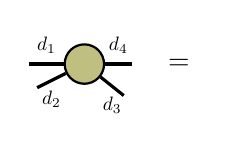
\begin{tikzpicture}[baseline=-0.5ex]
    \tikzset{tensor/.style = {minimum size = 0.5cm,shape = circle,thick,draw=black,inner sep = 0pt}, edge/.style = {thick,line width=.4mm},every loop/.style={}}
    \def\x{6}
    \def\y{0}   \node[tensor,fill=green!50!red!50!white] (T) at (\x+1,\y) {$\Tt$};
    \draw[edge] (T) -- (\x+0.3,0) node [midway,above] {\scalebox{0.7}{\dimcolor{$d_1$}}};
    \draw[edge] (T) -- (\x+1.6,0) node [midway,above] {\scalebox{0.7}{\dimcolor{$d_4$}}};;
    \draw[edge] (T) -- (\x+0.4,-0.3) node [midway, below] {\scalebox{0.7}{\dimcolor{$d_2$}}};
    \draw[edge] (T) -- (\x+1.5,-0.4)node [midway, below] {\scalebox{0.7}{\dimcolor{$d_3$}}};
    \node[draw = none] at (\x+2.2,0){$=$};
\end{tikzpicture}
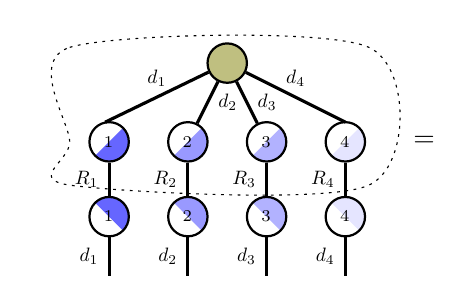
\begin{tikzpicture}[baseline=-0.5ex]
    \tikzset{tensor/.style = {minimum size = 0.5cm,shape = circle,thick,draw=black,inner sep = 0pt}, edge/.style = {thick,line width=.4mm},every loop/.style={}}
    \def\x{6}
    \def\y{0} 
    \node[tensor,fill=green!50!red!50!white] (T) at (\x+4.5,\y+1) {$\Tt$};
    \node[tensor, path picture={
    \fill[fill=blue!60!white](path picture bounding box.north east)
        -- 
    (path picture bounding box.south east) --
    (path picture bounding box.south west) -- cycle;
    }, shift={(\x+3,\y)}] (U_1) {\scalebox{0.85}{$\Ub_1$}};
    \node[tensor, path picture={
    \fill[fill=blue!60!white](path picture bounding box.south east)
        -- 
    (path picture bounding box.north east) --
    (path picture bounding box.north west) -- cycle;
    }, shift={(\x+3,\y-0.95)}] (Ut_1) {\scalebox{0.85}{$\Ub_1$}};
    \node[tensor, path picture={
    \fill[fill=blue!40!white](path picture bounding box.north east)
        -- 
    (path picture bounding box.south east) --
    (path picture bounding box.south west) -- cycle;
    }, shift={(\x+4,\y)}] (U_2) {\scalebox{0.85}{$\Ub_2$}};
    \node[tensor, path picture={
    \fill[fill=blue!40!white](path picture bounding box.south east)
        -- 
    (path picture bounding box.north east) --
    (path picture bounding box.north west) -- cycle;
    }, shift={(\x+4,\y-0.95)}] (Ut_2) {\scalebox{0.85}{$\Ub_2$}};
    \node[tensor, path picture={
    \fill[fill=blue!30!white](path picture bounding box.north east)
    -- 
    (path picture bounding box.south west) --
    (path picture bounding box.south east) -- cycle;
    }, shift={(\x+5,\y)}] (U_3) {\scalebox{0.85}{$\Ub_3$}};
    \node[tensor, path picture={
    \fill[fill=blue!30!white](path picture bounding box.south east)
        -- 
    (path picture bounding box.north east) --
    (path picture bounding box.north west) -- cycle;
    }, shift={(\x+5,\y-0.95)}] (Ut_3) {\scalebox{0.85}{$\Ub_3$}};
    \node[tensor, path picture={
    \fill[fill=blue!10!white](path picture bounding box.north east)
    -- 
    (path picture bounding box.south west) --
    (path picture bounding box.south east) -- cycle;
    }, shift={(\x+6,\y)}] (U_4) {\scalebox{0.85}{$\Ub_4$}};
    \node[tensor, path picture={
    \fill[fill=blue!10!white](path picture bounding box.south east)
        -- 
    (path picture bounding box.north east) --
    (path picture bounding box.north west) -- cycle;
    }, shift={(\x+6,\y-0.95)}] (Ut_4) {\scalebox{0.85}{$\Ub_4$}};
    \draw[edge] (T) -- (\x+2.95,\y+0.25) node [midway, above] {\scalebox{0.7}{\dimcolor{$d_1$}}};
    \draw[edge] (T) -- (U_2) node [midway, right] {\scalebox{0.7}{\dimcolor{$d_2$}}};
    \draw[edge] (T) -- (U_3) node [midway, right] {\scalebox{0.7}{\dimcolor{$d_3$}}};
    \draw[edge] (T) -- (\x+6,\y+0.25) node [midway, above] {\scalebox{0.7}{\dimcolor{$d_4$}}};
    \draw[edge] (U_1) -- (\x+3,\y-0.7) node [midway, left] {\scalebox{0.7}{\dimcolor{$R_1$}}};
    \draw[edge] (U_2) -- (\x+4,\y-0.7) node [midway, left] {\scalebox{0.7}{\dimcolor{$R_2$}}};
    \draw[edge] (U_3) -- (\x+5,\y-0.7) node [midway, left] {\scalebox{0.7}{\dimcolor{$R_3$}}};
    \draw[edge] (U_4) -- (\x+6,\y-0.7) node [midway, left] {\scalebox{0.7}{\dimcolor{$R_4$}}};
    \draw[edge] (Ut_1) -- (\x+3,\y-1.7) node [midway, left] {\scalebox{0.7}{\dimcolor{$d_1$}}};
    \draw[edge] (Ut_2) -- (\x+4,\y-1.7) node [midway, left] {\scalebox{0.7}{\dimcolor{$d_2$}}};
    \draw[edge] (Ut_3) -- (\x+5,\y-1.7) node [midway, left] {\scalebox{0.7}{\dimcolor{$d_3$}}};
    \draw[edge] (Ut_4) -- (\x+6,\y-1.7) node [midway, left] {\scalebox{0.7}{\dimcolor{$d_4$}}};
    \draw[dash pattern=on 1pt off 2pt] plot[smooth cycle] coordinates { 
    (\x+2.5,\y) 
    (\x+2.5, \y+1.2) (\x+6.3,\y+1.2) (\x+6.3, \y-0.55)  (\x+2.5,\y-0.55)};
    \node[draw = none] at (\x+7,0){$=$};
\end{tikzpicture}
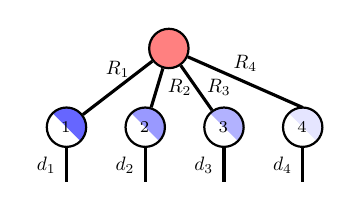
\begin{tikzpicture}[baseline=-0.5ex]
    \tikzset{tensor/.style = {minimum size = 0.5cm,shape = circle,thick,draw=black,inner sep = 0pt}, edge/.style = {thick,line width=.4mm},every loop/.style={}}
    \def\x{6}
    \def\y{0} 
    \node[tensor,fill=red!50!white] (G) at (\x+13.5,\y+1) {$\Gt$};
    \node[tensor, path picture={
    \fill[fill=blue!60!white](path picture bounding box.south east)
    -- 
    (path picture bounding box.north west) --
    (path picture bounding box.north east) -- cycle;
    }, shift={(\x+12.2,\y)}] (U_1)  {\scalebox{0.85}{$\Ub_1$}};  \node[tensor, path picture={
    \fill[fill=blue!40!white](path picture bounding box.south east)
    -- 
    (path picture bounding box.north west) --
    (path picture bounding box.north east) -- cycle;
    }, shift={(\x+13.2,\y)}] (U_2) {\scalebox{0.85}{$\Ub_2$}};
    \node[tensor, path picture={
    \fill[fill=blue!30!white](path picture bounding box.south east)
    -- 
    (path picture bounding box.north west) --
    (path picture bounding box.north east) -- cycle;
    }, shift={(\x+14.2,\y)}] (U_3) {\scalebox{0.85}{$\Ub_3$}};
        \node[tensor, path picture={
    \fill[fill=blue!10!white](path picture bounding box.south east)
    -- 
    (path picture bounding box.north west) --
    (path picture bounding box.north east) -- cycle;
    }, shift={(\x+15.2,\y)}] (U_4) {\scalebox{0.85}{$\Ub_4$}};
     \draw[edge] (U_1) -- (\x+12.2,\y-0.7) node [midway, left] {\scalebox{0.7}{\dimcolor{$d_1$}}};
    \draw[edge] (U_2) -- (\x+13.2,\y-0.7) node [midway, left] {\scalebox{0.7}{\dimcolor{$d_2$}}};
    \draw[edge] (U_3) -- (\x+14.2,\y-0.7) node [midway, left] {\scalebox{0.7}{\dimcolor{$d_3$}}};
    \draw[edge] (U_4) -- (\x+15.2,\y-0.7) node [midway, left] {\scalebox{0.7}{\dimcolor{$d_4$}}};
    \draw[edge](G) -- (U_1)node[midway,above]{\scalebox{0.7}{\dimcolor{$R_1$}}};
    \draw[edge](G) -- (U_2)node[midway,right]{\scalebox{0.7}{\dimcolor{$R_2$}}};
    \draw[edge](G) -- (U_3)node[midway,right]{\scalebox{0.7}{\dimcolor{$R_3$}}};
    \draw[edge](G) -- (\x+15.2,\y+0.25)node[midway,above]{\scalebox{0.7}{\dimcolor{$R_4$}}};
\end{tikzpicture}.
$$
where the tensor $\Gt = \Tt\ttm{1}\Ub_1^\ts\ttm{2}\dots\ttm{4}\Ub_4^\ts$. 

The core tensor  $\Gt\in\RR^{R_1\times\dots\times R_4}$ along with the factor matrices $\Ub_1,\dots,\Ub_4$ forms a Tucker decomposition of the tensor $\Tt$. If all the SVDs of the matricization of $\Tt$ are exact, the resulting Tucker decomposition will be exact as well. When using truncated SVDs, the overall approximation error of the Tucker decomposition can be expressed as a function of the errors made in each truncated SVD~(see~\citep{de2000multilinear}).

\paragraph{Multi-linear rank and rank of matricizations}
The algorithm above shows that, if $\tilde R_n = \rank(\Tt_{(n)})$ for all $n$, then there exists a Tucker decomposition of rank $(\tilde R_1,\dots, \tilde R_N)$, showing that the multi-linear rank $( R_1,\dots, R_N)$ of $\Tt$ is upper bounded by the rank of the matricizations: $ R_n \leq \rank(\Tt_{(n)} )$ for all $n$. It is also easy to show that the multi-linear rank is lower bounded by the rank of the matricizations. Indeed, suppose $\T$ has multi-linear rank-$(R_1,\dots, R_N)$. Then, there exists a rank-$(R_1,\dots, R_N)$ Tucker decomposition $\Tt = \Gt\times_1\Ub_1\times_2 \dots \times_N \Ub_N$. Using Theorem~\ref{thm: matricization-rank}, we can easily see that this implies $\rank(\Tt_{(n)} )\leq  R_n$ for all $n$.
This proves the following theorem.
\begin{theorem}
The multi-linear rank-$(R_1,R_2,\dots, R_N)$ of a tensor $\Tt$ is given by the rank of its matricizations, i.e., $R_n = \rank(\Tt_{(n)})$ for $n\in[N]$.
\end{theorem}


\begin{remark}\label{rem:tuckers}
We list here some interesting properties of the Tucker decomposition and the Higher-Order SVD~(HOSVD) algorithm for computing it.
\begin{enumerate}

\item  If  $\Tt = \Gt\ttm{1}\Ub_1\ttm{2}\dots\ttm{N-1}\Ub_{N-1}\ttm{N}\Ub_N$ with all the $\Ub_i$ orthogonal, then $\norm{\Tt}_F = \norm{\Gt}_F$ and $\vectorize(\Gt) = (\Ub_1\kron\cdots\kron\Ub_N)\vectorize(\Tt)$. 
Indeed, for $N=3$ we have
\begin{align*}
(\Ub_1\kron\Ub_2\kron\Ub_3)\vectorize(\Tt) &= 
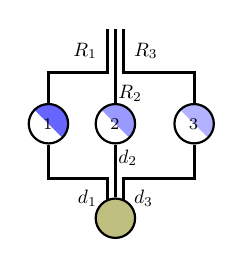
\begin{tikzpicture}[baseline=-0.5ex]
    \tikzset{tensor/.style = {minimum size = 0.5cm,shape = circle,thick,draw=black,inner sep = 0pt}, edge/.style = {thick,line width=.4mm},every loop/.style={}}
    \def\x{0}
    \def\y{0.5}   
    \node[tensor, path picture={
    \fill[fill=blue!60!white](path picture bounding box.south east)
        -- 
    (path picture bounding box.north west) --
    (path picture bounding box.north east) -- cycle;
    }, shift={(\x-0.85,\y-0.65)}] (U_1) {\scalebox{0.85}{$\Ub_1$}};
    \node[tensor, path picture={
    \fill[fill=blue!40!white](path picture bounding box.south east)
        -- 
    (path picture bounding box.north west) --
    (path picture bounding box.north east) -- cycle;
    }, shift={(\x,\y-0.65)}] (U_2) {\scalebox{0.85}{$\Ub_2$}};
    \node[tensor, path picture={
    \fill[fill=blue!30!white](path picture bounding box.south east)
        -- 
    (path picture bounding box.north west) --
    (path picture bounding box.north east) -- cycle;
    }, shift={(\x+1,\y-0.65)}] (U_3) {\scalebox{0.85}{$\Ub_3$}};
    \draw[edge] (U_1) -- (\x-0.85,\y-1.35) -- (\x-0.1,\y-1.35) -- (\x-0.1,\y-1.85) node [midway, left] {\scalebox{0.7}{\dimcolor{$d_1$}}};
    \draw[edge] (U_2) -- (\x,\y+0.55) node [very near start, right=-0.1cm] {\scalebox{0.7}{\dimcolor{$R_2$}}};
    \draw[edge] (U_3) -- (\x+1,\y-1.35) -- (\x+0.1,\y-1.35) -- (\x+0.1, \y-1.85) node [midway, right] {\scalebox{0.7}{\dimcolor{$d_3$}}};
    \draw[edge](U_1) -- (\x-0.85,\y) -- (\x-0.1,\y) -- (\x-0.1,\y+0.55)node [midway, left] {\scalebox{0.7}{\dimcolor{$R_1$}}};
    \draw[edge](U_3) -- (\x+1,\y) -- (\x+0.1,\y) -- (\x+0.1,\y+0.55)node [midway, right] {\scalebox{0.7}{\dimcolor{$R_3$}}};
    \node[tensor,fill=green!50!red!50!white](T) at (\x,\y-1.85) {$\Tt$};
    \draw[edge](U_2)--(T)node [near start, right=-0.1cm] {\scalebox{0.7}{\dimcolor{$d_2$}}};
\end{tikzpicture}
=
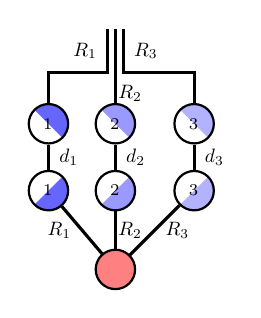
\begin{tikzpicture}[baseline=-0.5ex]
    \tikzset{tensor/.style = {minimum size = 0.5cm,shape = circle,thick,draw=black,inner sep = 0pt}, edge/.style = {thick,line width=.4mm},every loop/.style={}}
    \def\x{0}
    \def\y{1.25}   
    \node[tensor, path picture={
    \fill[fill=blue!60!white](path picture bounding box.south east)
        -- 
    (path picture bounding box.north west) --
    (path picture bounding box.north east) -- cycle;
    }, shift={(\x-0.85,\y-0.65)}] (U_1) {\scalebox{0.85}{$\Ub_1$}};
    \node[tensor, path picture={
    \fill[fill=blue!60!white](path picture bounding box.north east)
        -- 
    (path picture bounding box.south west) --
    (path picture bounding box.south east) -- cycle;
    }, shift={(\x-0.85,\y-1.5)}] (Ut_1) {\scalebox{0.85}{$\Ub_1$}};
    \node[tensor, path picture={
    \fill[fill=blue!40!white](path picture bounding box.south east)
        -- 
    (path picture bounding box.north west) --
    (path picture bounding box.north east) -- cycle;
    }, shift={(\x,\y-0.65)}] (U_2) {\scalebox{0.85}{$\Ub_2$}};
     \node[tensor, path picture={
    \fill[fill=blue!40!white](path picture bounding box.north east)
        -- 
    (path picture bounding box.south west) --
    (path picture bounding box.south east) -- cycle;
    }, shift={(\x,\y-1.5)}] (Ut_2) {\scalebox{0.85}{$\Ub_2$}};
    \node[tensor, path picture={
    \fill[fill=blue!30!white](path picture bounding box.south east)
        -- 
    (path picture bounding box.north west) --
    (path picture bounding box.north east) -- cycle;
    }, shift={(\x+1,\y-0.65)}] (U_3) {\scalebox{0.85}{$\Ub_3$}};
    \node[tensor, path picture={
    \fill[fill=blue!30!white](path picture bounding box.north east)
        -- 
    (path picture bounding box.south west) --
    (path picture bounding box.south east) -- cycle;
    }, shift={(\x+1,\y-1.5)}] (Ut_3) {\scalebox{0.85}{$\Ub_3$}};
    \draw[edge] (U_2) -- (\x,\y+0.55) node [very near start, right=-0.1cm] {\scalebox{0.7}{\dimcolor{$R_2$}}};
    \draw[edge](U_1) -- (\x-0.85,\y) -- (\x-0.1,\y) -- (\x-0.1,\y+0.55)node [midway, left] {\scalebox{0.7}{\dimcolor{$R_1$}}};
    \draw[edge](U_3) -- (\x+1,\y) -- (\x+0.1,\y) -- (\x+0.1,\y+0.55)node [midway, right] {\scalebox{0.7}{\dimcolor{$R_3$}}};
    \draw[edge](U_1)--(Ut_1)node [midway, right] {\scalebox{0.7}{\dimcolor{$d_1$}}};
    \draw[edge](U_2)--(Ut_2)node [midway, right] {\scalebox{0.7}{\dimcolor{$d_2$}}};
    \draw[edge](U_3)--(Ut_3)node [midway, right] {\scalebox{0.7}{\dimcolor{$d_3$}}};
    \node[tensor,fill=red!50!white] (G) at (\x,\y-2.5) {$\Gt$};
    \draw[edge](G)--(Ut_1)node [midway, left] {\scalebox{0.7}{\dimcolor{$R_1$}}};
    \draw[edge](G)--(Ut_2)node [midway, right=-0.1cm] {\scalebox{0.7}{\dimcolor{$R_2$}}};
    \draw[edge](G)--(Ut_3)node [midway, right] {\scalebox{0.7}{\dimcolor{$R_3$}}};
\end{tikzpicture}
=
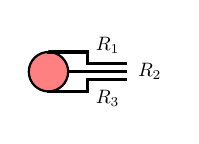
\begin{tikzpicture}[baseline=-0.5ex]
    \tikzset{tensor/.style = {minimum size = 0.5cm,shape = circle,thick,draw=black,inner sep = 0pt}, edge/.style = {thick,line width=.4mm},every loop/.style={}}
    \def\x{6}
    \def\y{0}
    \node[tensor,fill=red!50!white] (G) at (\x+4.5,\y) {$\Gt$};
    \draw[edge](G) -- (\x+5.5,\y) node [right] {\scalebox{0.7}{\dimcolor{$R_2$}}};
    \draw[edge](G) -- (\x+4.5,\y+0.25) -- (\x+5,\y+0.25) -- (\x+5,\y+0.1) -- (\x+5.5, \y+0.1) node [midway,above] {\scalebox{0.7}{\dimcolor{$R_1$}}};
    \draw[edge](G) -- (\x+4.5,\y-0.25) -- (\x+5,\y-0.25) -- (\x+5,\y-0.1) -- (\x+5.5, \y-0.1) node [midway,below] {\scalebox{0.7}{\dimcolor{$R_3$}}};
    \end{tikzpicture}
    =\vectorize(\Gt).
\end{align*}

Observing that $\Ub_1\kron\Ub_2\kron\Ub_3$ is a left-orthogonal matrix, it follows that 
 $\norm{\Tt} = \norm{\vectorize(\Tt)} = \norm{(\Ub_1\kron\Ub_2\kron\Ub_3)\vectorize(\Tt)}= \norm{\vectorize(\Gt)} = \norm{\Gt}$.
    


    \item If we do not enforce any orthogonality constraints on the factor matrices and fix the core tensor to be a copy tensor,
$
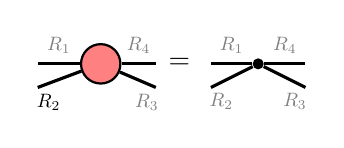
\begin{tikzpicture}[baseline=-0.5ex]
    \tikzset{tensor/.style = {minimum size = 0.5cm,shape = circle,thick,draw=black,inner sep = 0pt}, edge/.style = {thick,line width=.4mm},every loop/.style={}}
    \def\x{6}
    \def\y{0}
    \node[tensor,fill=red!50!white] (G) at (\x+4.5,\y) {$\Gt$};
    \draw[edge] (G) -- (\x+5.2,\y) node [midway, above] {\scalebox{0.7}{\textcolor{gray}{$R_4$}}};
    \draw[edge] (G) -- (\x+3.7,\y-0.3) node [below, near end] {\scalebox{0.7}{\dimcolor{$R_2$}}};
    \draw[edge] (G) -- (\x+5.2,\y-0.3) node [below, near end] {\scalebox{0.7}{\textcolor{gray}{$R_3$}}};
    \draw[edge] (G) -- (\x+3.7,\y) node [midway, above] {\scalebox{0.7}{\textcolor{gray}{$R_1$}}};
    \node[draw = none] at (\x+5.5,0){$=$};
    \draw  node[fill = black,circle,inner sep=0pt,minimum size=4pt] (m) at (\x+6.5,\y) {};
    \draw[edge] (m) -- (\x+7.1,\y) node [midway, above] {\scalebox{0.7}{\textcolor{gray}{$R_4$}}};
    \draw[edge] (m) -- (\x+5.9,\y-0.3) node [below, near end] {\scalebox{0.7}{\textcolor{gray}{$R_2$}}};
    \draw[edge] (m) -- (\x+7.1,\y-0.3) node [below, near end] {\scalebox{0.7}{\textcolor{gray}{$R_3$}}};
    \draw[edge] (m) -- (\x+5.9,\y) node [midway, above] {\scalebox{0.7}{\textcolor{gray}{$R_1$}}};
\end{tikzpicture},
$
we recover the CP decomposition. %
    \item \label{item:Tucker_orth} If $\Tt = \Gt\ttm{1}\Ab_1\ttm{2}\Ab_2\ttm{3}\Ab_3\ttm{4}\Ab_4$, with $\Ab_1,\Ab_2,\Ab_3$ and $\Ab_4$ not necessarily orthogonal, then there exists $\Tilde{\Gt}$ (of the same size as $\Gt$) and $\Qb_1,\Qb_2,\Qb_3$ and $\Qb_4$ orthogonal such that $\Tt = \Tilde{\Gt}\ttm{1}\Qb_1\ttm{2}\Qb_2\ttm{3}\Qb_3\ttm{4}\Qb_4$.
    \begin{proof}
By performing QR decomposition on each factor matrix, we obtain
\begin{align*}
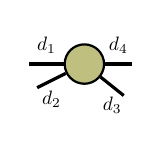
\begin{tikzpicture}[baseline=-0.5ex]
    \tikzset{tensor/.style = {minimum size = 0.5cm,shape = circle,thick,draw=black,inner sep = 0pt}, edge/.style = {thick,line width=.4mm},every loop/.style={}}
    \def\x{6}
    \def\y{0}   \node[tensor,fill=green!50!red!50!white] (T) at (\x+1,\y) {$\Tt$};
    \draw[edge] (T) -- (\x+0.3,0) node [midway,above] {\scalebox{0.7}{\dimcolor{$d_1$}}};
    \draw[edge] (T) -- (\x+1.6,0) node [midway,above] {\scalebox{0.7}{\dimcolor{$d_4$}}};;
    \draw[edge] (T) -- (\x+0.4,-0.3) node [midway, below] {\scalebox{0.7}{\dimcolor{$d_2$}}};
    \draw[edge] (T) -- (\x+1.5,-0.4)node [midway, below] {\scalebox{0.7}{\dimcolor{$d_3$}}};
\end{tikzpicture}
&=
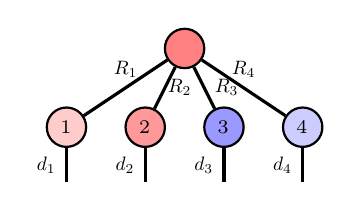
\begin{tikzpicture}[baseline=-0.5ex]
    \tikzset{tensor/.style = {minimum size = 0.5cm,shape = circle,thick,draw=black,inner sep = 0pt}, edge/.style = {thick,line width=.4mm},every loop/.style={}}
    \def\x{6}
    \def\y{0}   
    \node[tensor,fill=red!50!white] (G) at (\x+4.5,\y+1) {$\Gt$};
    \node[tensor,fill=red!20!white] (A_1) at (\x+3,\y){$\Ab_1$};
    \node[tensor,fill=red!40!white] (A_2) at (\x+4,\y){$\Ab_2$};
    \node[tensor, fill=blue!40!white] (A_3) at (\x+5,\y){$\Ab_3$};
    \node[tensor,fill=blue!20!white] (A_4) at (\x+6,\y){$\Ab_4$};
    \draw[edge] (G) -- (A_1) node [midway, above] {\scalebox{0.7}{\dimcolor{$R_1$}}};
    \draw[edge] (G) -- (A_2) node [midway, right=-0.1cm] {\scalebox{0.7}{\dimcolor{$R_2$}}};
    \draw[edge] (G) -- (A_3) node [midway, right=-0.05] {\scalebox{0.7}{\dimcolor{$R_3$}}};
    \draw[edge] (G) -- (A_4) node [midway, above] {\scalebox{0.7}{\dimcolor{$R_4$}}};
    \draw[edge] (A_1) -- (\x+3,\y-0.7) node [midway, left] {\scalebox{0.7}{\dimcolor{$d_1$}}};
    \draw[edge] (A_2) -- (\x+4,\y-0.7) node [midway, left] {\scalebox{0.7}{\dimcolor{$d_2$}}};
    \draw[edge] (A_3) -- (\x+5,\y-0.7) node [midway, left] {\scalebox{0.7}{\dimcolor{$d_3$}}};
    \draw[edge] (A_4) -- (\x+6,\y-0.7) node [midway, left] {\scalebox{0.7}{\dimcolor{$d_4$}}};
\end{tikzpicture}\\
&=
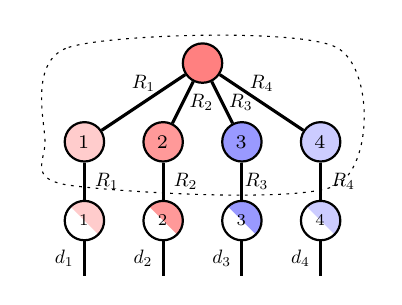
\begin{tikzpicture}[baseline=-0.5ex]
    \tikzset{tensor/.style = {minimum size = 0.5cm,shape = circle,thick,draw=black,inner sep = 0pt}, edge/.style = {thick,line width=.4mm},every loop/.style={}}
    \def\x{6}
    \def\y{0}   
   \node[tensor,fill=red!50!white] (G) at (\x+9,\y+1) {$\Gt$};
    \node[tensor,fill=red!20!white] (R_1) at (\x+7.5,\y){$\Rb_1$};
    \node[tensor,fill=red!40!white] (R_2) at (\x+8.5,\y){$\Rb_2$};
    \node[tensor, fill=blue!40!white] (R_3) at (\x+9.5,\y){$\Rb_3$};
    \node[tensor,fill=blue!20!white] (R_4) at (\x+10.5,\y){$\Rb_4$};
    \node[tensor, path picture={
    \fill[fill=red!20!white](path picture bounding box.south east)
    -- 
    (path picture bounding box.north west) --
    (path picture bounding box.north east) -- cycle;
    }, shift={(\x+7.5,\y-1)}] (Q_1)  {\scalebox{0.85}{$\Qb_1$}};  \node[tensor, path picture={
    \fill[fill=red!40!white](path picture bounding box.south east)
    -- 
    (path picture bounding box.north west) --
    (path picture bounding box.north east) -- cycle;
    }, shift={(\x+8.5,\y-1)}] (Q_2) {\scalebox{0.85}{$\Qb_2$}};
    \node[tensor, path picture={
    \fill[fill=blue!40!white](path picture bounding box.south east)
    -- 
    (path picture bounding box.north west) --
    (path picture bounding box.north east) -- cycle;
    }, shift={(\x+9.5,\y-1)}] (Q_3) {\scalebox{0.85}{$\Qb_3$}};
        \node[tensor, path picture={
    \fill[fill=blue!20!white](path picture bounding box.south east)
    -- 
    (path picture bounding box.north west) --
    (path picture bounding box.north east) -- cycle;
    }, shift={(\x+10.5,\y-1)}] (Q_4) {\scalebox{0.85}{$\Qb_4$}};
    \draw[edge] (G) -- (R_1) node [midway, above] {\scalebox{0.7}{\dimcolor{$R_1$}}};
    \draw[edge] (G) -- (R_2) node [midway, right=-0.05cm] {\scalebox{0.7}{\dimcolor{$R_2$}}};
    \draw[edge] (G) -- (R_3) node [midway, right=-0.05cm] {\scalebox{0.7}{\dimcolor{$R_3$}}};
    \draw[edge] (G) -- (R_4) node [midway, above] {\scalebox{0.7}{\dimcolor{$R_4$}}};
    \draw[edge] (R_1) -- (Q_1) node [midway, right] {\scalebox{0.7}{\dimcolor{$R_1$}}};
    \draw[edge] (R_2) -- (Q_2) node [midway, right] {\scalebox{0.7}{\dimcolor{$R_2$}}};
    \draw[edge] (R_3) -- (Q_3) node [midway, right=-0.1cm] {\scalebox{0.7}{\dimcolor{$R_3$}}};
    \draw[edge] (R_4) -- (Q_4) node [midway, right] {\scalebox{0.7}{\dimcolor{$R_4$}}};
    \draw[edge] (Q_1) -- (\x+7.5,\y-1.7) node [midway, left] {\scalebox{0.7}{\dimcolor{$d_1$}}};
    \draw[edge] (Q_2) -- (\x+8.5,\y-1.7) node [midway, left] {\scalebox{0.7}{\dimcolor{$d_2$}}};
    \draw[edge] (Q_3) -- (\x+9.5,\y-1.7) node [midway, left] {\scalebox{0.7}{\dimcolor{$d_3$}}};
    \draw[edge] (Q_4) -- (\x+10.5,\y-1.7) node [midway, left] {\scalebox{0.7}{\dimcolor{$d_4$}}};
    \draw[dash pattern=on 1pt off 2pt] plot[smooth cycle] coordinates { 
    (\x+7,\y) 
    (\x+7.3, \y+1.2) (\x+10.7,\y+1.2) (\x+10.7, \y-0.55)  (\x+7.3,\y-0.55)};
\end{tikzpicture}
=
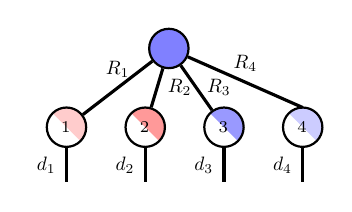
\begin{tikzpicture}[baseline=-0.5ex]
    \tikzset{tensor/.style = {minimum size = 0.5cm,shape = circle,thick,draw=black,inner sep = 0pt}, edge/.style = {thick,line width=.4mm},every loop/.style={}}
    \def\x{6}
    \def\y{0}   
    \node[tensor,fill=blue!50!white] (G) at (\x+13.5,\y+1) {$\Tilde{\Gt}$};
    \node[tensor, path picture={
    \fill[fill=red!20!white](path picture bounding box.south east)
    -- 
    (path picture bounding box.north west) --
    (path picture bounding box.north east) -- cycle;
    }, shift={(\x+12.2,\y)}] (Q_1)  {\scalebox{0.85}{$\Qb_1$}};  \node[tensor, path picture={
    \fill[fill=red!40!white](path picture bounding box.south east)
    -- 
    (path picture bounding box.north west) --
    (path picture bounding box.north east) -- cycle;
    }, shift={(\x+13.2,\y)}] (Q_2) {\scalebox{0.85}{$\Qb_2$}};
    \node[tensor, path picture={
    \fill[fill=blue!40!white](path picture bounding box.south east)
    -- 
    (path picture bounding box.north west) --
    (path picture bounding box.north east) -- cycle;
    }, shift={(\x+14.2,\y)}] (Q_3) {\scalebox{0.85}{$\Qb_3$}};
        \node[tensor, path picture={
    \fill[fill=blue!20!white](path picture bounding box.south east)
    -- 
    (path picture bounding box.north west) --
    (path picture bounding box.north east) -- cycle;
    }, shift={(\x+15.2,\y)}] (Q_4) {\scalebox{0.85}{$\Qb_4$}};
     \draw[edge] (Q_1) -- (\x+12.2,\y-0.7) node [midway, left] {\scalebox{0.7}{\dimcolor{$d_1$}}};
    \draw[edge] (Q_2) -- (\x+13.2,\y-0.7) node [midway, left] {\scalebox{0.7}{\dimcolor{$d_2$}}};
    \draw[edge] (Q_3) -- (\x+14.2,\y-0.7) node [midway, left] {\scalebox{0.7}{\dimcolor{$d_3$}}};
    \draw[edge] (Q_4) -- (\x+15.2,\y-0.7) node [midway, left] {\scalebox{0.7}{\dimcolor{$d_4$}}};
    \draw[edge](G) -- (Q_1)node[midway,above]{\scalebox{0.7}{\dimcolor{$R_1$}}};
    \draw[edge](G) -- (Q_2)node[midway,right]{\scalebox{0.7}{\dimcolor{$R_2$}}};
    \draw[edge](G) -- (Q_3)node[midway,right]{\scalebox{0.7}{\dimcolor{$R_3$}}};
    \draw[edge](G) -- (\x+15.2,\y+0.25)node[midway,above]{\scalebox{0.7}{\dimcolor{$R_4$}}};
\end{tikzpicture}.
\end{align*}
\end{proof}
\item For an $N$-th order $d$-dimensional tensor, the number of parameters in its Tucker decomposition is $\bigo(R^N+NdR)$ assuming $R_1=\dots=R_N=R$.
\item
We conclude this section by showing how the mode-$n$ matricization of the Tucker decomposition of a tensor can be expressed using Kronecker products.
\begin{proposition}\label{decomp:tucker-kron}
Let $\At\in\RR^{d_1\times d_2\times\dots\times d_N}$. If $\At=\Gt\ttm{1}\Ub_1\ttm{2}\dots\ttm{N}\Ub_N$ then
$$\At_{(i)}=\Ub_i\Gt_{(i)}\left(\Ub_1\kron\dots\kron\Ub_{(i-1)}\kron\Ub_{(i+1)}\kron\dots\kron\Ub_N\right)^\ts.$$
\begin{proof}
Assume $N=3$ and $n=1$, then we obtain
\begin{align*}
\At_{(1)}
&=
\left(\begin{tikzpicture}[baseline=\baseline]
    \tikzset{tensor/.style = {minimum size = 0.5cm,shape = circle,thick,draw=black,inner sep = 0pt}, edge/.style  = {thick,line width=.4mm},every loop/.style={}}
    \def\y{0}
    \def\x{0}
    \node[tensor,fill=green!50!red!50!white] (At) at (\x,\y){\scalebox{0.85}{$\At$}};
    \draw[edge] (\x+0.25,\y) -- (\x+0.6,\y)  node [midway,above] {\scalebox{0.7}{\dimcolor{$d_2$}}};
    \draw[edge] (\x-0.25,\y) -- (\x-0.6,\y)  node [midway,above] {\scalebox{0.7}{\dimcolor{$d_1$}}};
    \draw[edge] (\x,\y-0.25) -- (\x,\y-0.7)  node [midway,left] {\scalebox{0.7}{\dimcolor{$d_3$}}};
    \end{tikzpicture}\right)_{(1)}
=
\left(\begin{tikzpicture}[baseline=\baseline]
    \tikzset{tensor/.style = {minimum size = 0.5cm,shape = circle,thick,draw=black,inner sep = 0pt}, edge/.style   = {thick,line width=.4mm},every loop/.style={}}
    \def\y{0}
    \def\x{0}
  \node[tensor,fill=red!50!white] (A1) at (\x,\y){\scalebox{0.85}{$\Ub_1$}};
  \node[tensor,fill=blue!50!white] (A2) at (\x+1,\y){$\Ub_2$};
   \node[tensor,fill=blue!20!white] (A3) at (\x+2,\y){$\Ub_3$};
   \node[tensor,fill=red!60!blue!20!white] (m) at (\x+1,\y+1) {$\Gt$};
    \draw[edge] (A1) -- (m)node [midway,left] {\scalebox{0.7}{\dimcolor{$R_1$}}};
    \draw[edge] (A2) -- (m)node [midway,right=-0.05cm] {\scalebox{0.7}{\dimcolor{$R_2$}}};
    \draw[edge] (A3) -- (m)node [midway,right] {\scalebox{0.7}{\dimcolor{$R_3$}}};
    \draw[edge](A1) -- (\x,\y-0.7)node [midway,left] {\edgelabel{$d_1$}};
    \draw[edge](A2) -- (\x+1,\y-0.7)node [midway,left] {\edgelabel{$d_2$}};
    \draw[edge](A3) -- (\x+2,\y-0.7)node [midway,left] {\edgelabel{$d_3$}};
\end{tikzpicture}\right)_{(1)}\\
&=
\begin{tikzpicture}[baseline=\baseline]
    \tikzset{tensor/.style = {minimum size = 0.5cm,shape = circle,thick,draw=black,inner sep = 0pt}, edge/.style   = {thick,line width=.4mm},every loop/.style={}}
    \def\y{0}
    \def\x{0}
    \node[tensor,fill=green!50!red!50!white] (At) at (\x,\y){\scalebox{0.85}{$\At$}};
    \draw[edge] (\x-0.25,\y) -- (\x-0.6,\y)  node [midway,above] {\scalebox{0.7}{\dimcolor{$d_1$}}};
    \draw[edge] (\x+0.2,\y+0.15) -- (\x+0.5,\y+0.15)-- (\x+0.5,\y+0.05) -- (\x+1,\y+0.05) node [midway,above]
    {\scalebox{0.7}{\dimcolor{$d_2$}}};
    \draw[edge] (\x+0.2,\y-0.15) -- (\x+0.5,\y-0.15)-- (\x+0.5,\y-0.05)-- (\x+1,\y-0.05) node [midway,below]
    {\scalebox{0.7}{\dimcolor{$d_3$}}};
    \end{tikzpicture}
=
\begin{tikzpicture}[baseline=\baseline]
    \tikzset{tensor/.style = {minimum size = 0.5cm,shape = circle,thick,draw=black,inner sep = 0pt}, edge/.style   = {thick,line width=.4mm},every loop/.style={}}
    \def\y{0}
    \def\x{0}
    \node[tensor,fill=red!50!white] (A1) at (\x,\y){\scalebox{0.85}{$\Ub_1$}};
    \node[tensor,fill=blue!50!white] (A2) at (\x+2.7,\y+0.7){$\Ub_2$};
    \node[tensor,fill=blue!20!white] (A3) at (\x+2.7,\y-0.7){$\Ub_3$};
    \node[tensor,fill=red!60!blue!20!white] (m) at (\x+1,\y) {$\Gt$}; 
     \draw[edge] (\x+1.2,\y+0.15) -- (\x+1.5,\y+0.15)-- (\x+1.5,\y+0.05) -- (\x+2,\y+0.05) node [midway,above]
    {\scalebox{0.7}{\dimcolor{$R_2$}}};
    \draw[edge] (\x+1.2,\y-0.15) -- (\x+1.5,\y-0.15)-- (\x+1.5,\y-0.05)-- (\x+2,\y-0.05) node [midway,below]
    {\scalebox{0.7}{\dimcolor{$R_3$}}};
    \draw[edge] (A1) -- (m) node [midway,above] {\scalebox{0.7}{\dimcolor{$R_1$}}};
    \draw[edge] (A1) -- (\x-0.7,\y) node [midway,above] {\scalebox{0.7}{\dimcolor{$d_1$}}};
    \draw[edge](\x+2,\y-0.05) -- (\x+2,\y-0.7) -- (A3);
    \draw[edge](\x+2,\y+0.05) -- (\x+2,\y+0.7) -- (A2);
    \draw[edge] (A2) -- (\x+3.5,\y+0.7) -- (\x+3.5,\y+0.05)-- (\x+4,\y+0.05) node [midway,above]
    {\scalebox{0.7}{\dimcolor{$d_2$}}};
    \draw[edge] (A3) -- (\x+3.5,\y-0.7) -- (\x+3.5,\y-0.05) -- (\x+4,\y-0.05) node [midway,below]
    {\scalebox{0.7}{\dimcolor{$d_3$}}};
    \end{tikzpicture}
=
\Ub_1\Gt_{(1)}(\Ub_2\kron\Ub_3)^\ts.
\end{align*}
\end{proof}
\end{proposition}
\end{enumerate}
\end{remark}
\subsection{Tensor Train~(TT) Decomposition}\label{sec:tt-decomposition}
The Tensor Train~(TT) decomposition~\citep{oseledets2010approximation} is another popular tensor factorization model. It decomposes an $N$-th order tensor into $N$ smaller third-order tensors. 
A rank-$(R_1,\dots,R_{N-1})$ \textit{tensor train decomposition} of a tensor $\St\in\RR^{d_1\times\cdots\times d_N}$ factorizes it into a product of $N$  third-order tensors\footnote{The first and last cores can be though as matrices rather than third-order tensors since they have a singleton dimension. However, considering them as third-rd order tensors allows us to lighten some notations.}, $\Gt_n\in\RR^{R_{n-1}\times d_n\times R_n}$ for $n\in [N]$, with $R_0=R_N=1$:
$$\St_{i_1,\cdots,i_N}= \sum_{r_0=1}^{R_0}\sum_{r_1=1}^{R_1} \cdots \sum_{r_{N-1}=1}^{R_{N-1}}\sum_{r_N=1}^{R_N} \prod_{n=1}^N\Gt_n(r_{n-1},i_n,r_n) := \TT(({\Gt_n})_{n=1}^N),$$ 
for all $i_1\in[d_1],\cdots,i_N\in[d_N]$.  
The \emph{TT-rank} of $\St$ is the smallest
$(R_1,R_2,\dots,R_{N-1})$ such that $\St$ admits an exact rank-$(R_1,R_2,\dots,R_{N-1})$ TT-decomposition $\St=\TT(({\Gt_n})_{n=1}^N)$.
Similarly to the CP and Tucker decomposition, the rank can be viewed as a hyperparameter that controls the expressivity of the TT decomposition. That is, with a sufficiently large rank, a TT decomposition can represent any arbitrary tensor. The following tensor network illustrates the rank-$(R_1,R_2,R_3)$ TT decomposition of a fourth-order tensor: 

$$
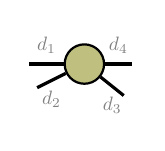
\begin{tikzpicture}[baseline=-0.5ex]
    \tikzset{tensor/.style = {minimum size = 0.5cm,shape = circle,thick,draw=black,inner sep = 0pt}, edge/.style = {thick,line width=.4mm},every loop/.style={}}
    \def\x{6}
    \def\y{0}
     \node[tensor,fill=green!50!red!50!white] (B) at (\x+1,\y) {$\St$};
    \draw[edge] (B) -- (\x+0.3,0) node [midway,above] {\scalebox{0.7}{\textcolor{gray}{$d_1$}}};
    \draw[edge] (B) -- (\x+1.6,0) node [midway,above] {\scalebox{0.7}{\textcolor{gray}{$d_4$}}};;
    \draw[edge] (B) -- (\x+0.4,-0.3) node [midway, below] {\scalebox{0.7}{\textcolor{gray}{$d_2$}}};;
    \draw[edge] (B) -- (\x+1.5,-0.4)node [midway, below] {\scalebox{0.7}{\textcolor{gray}{$d_3$}}};;
\end{tikzpicture}=
\begin{tikzpicture}[baseline=\baseline]
    \tikzset{tensor/.style = {minimum size = 0.5cm,shape = circle,thick,draw=black,inner sep = 0pt}, edge/.style   = {thick,line width=.4mm},every loop/.style={}}
    \def\y{0}
    \def\x{0}
  \node[tensor,fill=red!30!white] (D) at (\x-1,\y){$\Gt_1$};
  \node[tensor,fill=red!50!white] (A) at (\x,\y){\scalebox{0.85}{$\Gt_2$}};
  \node[tensor,fill=blue!50!white] (B) at (\x+1,\y){$\Gt_3$};
   \node[tensor,fill=blue!20!white] (C) at (\x+2,\y){$\Gt_4$};
    \draw[edge](A) -- (\x,\y-0.7)node [midway,left] {\edgelabel{$d_2$}};
    \draw[edge](B) -- (\x+1,\y-0.7)node [midway,left] {\edgelabel{$d_3$}};
    \draw[edge](C) -- (\x+2,\y-0.7)node [midway,left] {\edgelabel{$d_4$}};
     \draw[edge](D) -- (\x-1,\y-0.7)node [midway,left] {\edgelabel{$d_1$}};
    \draw[edge](D) -- (A) node [midway,above] {\edgelabel{$R_1$}};
    \draw[edge](A) -- (B) node [midway,above] {\edgelabel{$R_2$}};
    \draw[edge](B) -- (C) node [midway,above] {\edgelabel{$R_3$}};
\end{tikzpicture}.
$$
The TT decomposition was initially introduced in the quantum physics and condensed matter community as \emph{Matrix Product States~(MPS)}. In this context, the dimensions of the internal edges are referred to as \textit{bond dimensions}, and the free legs are called \textit{physical dimensions}.
Next, we show how an exact TT decomposition of a tensor $\St\in\RR^{d_1\times\dots\times d_N}$ can be computed in polynomial time using successive singular value decomposition (SVD). This algorithm is known as the TT-SVD algorithm~\citep{oseledets2010approximation}, but was introduced earlier in the quantum physics community and referred to as \textit{successive Schmidt decompositions}~\citep{vidal2004efficient,mcculloch2007density}. 
Before presenting the TT-SVD algorithm, we introduce the notions of left and right orthogonality for third-order tensors.
\begin{definition}\label{def:left-right-ortho}A core tensor $\At_n\in\RR^{R_{n-1}\times d_n\times R_n}$ for $n\in[N]$ is left-orthogonal if $(\At_n)_{(3)}^\ts(\At_n)_{(3)}=\Ib_{R_n}$ and right-orthogonal if $(\At_n)_{(1)}(\At_n)_{(1)}^\ts=\Ib_{R_{n-1}}$. This can be illustrated using tensor networks 
as follows:
\begin{align*}
\begin{tikzpicture}[baseline=\baseline]
    \tikzset{tensor/.style = {minimum size = 0.5cm,shape = circle,thick,draw=black,inner sep = 0pt}, edge/.style = {thick,line width=.4mm},every loop/.style={}}
    \def\y{0}
    \def\x{0}
    \node[tensor, path picture={
    \fill[fill=red!30!white](path picture bounding box.south east)
        -- 
    (path picture bounding box.north west) --
    (path picture bounding box.north east) -- cycle;
    }, shift={(\x,\y)}] (A) {\scalebox{0.85}{$\At_n$}};
    \draw[edge](A) -- (\x,\y-0.7)node [midway,left] {\scalebox{0.7}{\dimcolor{$d_n$}}};
    \draw[edge](A) -- (\x-0.85,\y)node [midway,above] {\scalebox{0.7}{\dimcolor{$R_{n-1}$}}};
    \draw[edge](A) -- (\x+0.85,\y)node [midway,above] {\scalebox{0.7}{\dimcolor{$R_n$}}};
\end{tikzpicture}\ \  \text{is left-orthogonal}
\iff
\begin{tikzpicture}[baseline=\baseline]
    \tikzset{tensor/.style = {minimum size = 0.5cm,shape = circle,thick,draw=black,inner sep = 0pt}, edge/.style = {thick,line width=.4mm},every loop/.style={}}
    \def\y{0}
    \def\x{0}
    \node[tensor, path picture={
    \fill[fill=red!30!white](path picture bounding box.south west)
        -- 
    (path picture bounding box.north east) --
    (path picture bounding box.north west) -- cycle;
    }, shift={(\x,\y)}] (A1) {\scalebox{0.85}{$\At_n$}};
    \node[tensor, path picture={
    \fill[fill=red!30!white](path picture bounding box.south east)
        -- 
    (path picture bounding box.north west) --
    (path picture bounding box.north east) -- cycle;
    }, shift={(\x+1,\y)}] (A2) {\scalebox{0.85}{$\At_n$}};
    \draw[edge](A1)--(A2)node [midway,above] {\scalebox{0.7}{\dimcolor{$R_{n-1}$}}};
    \draw[edge](\x+0.23,\y-0.1) -- (\x+0.77,\y-0.1) node [midway,below] {\scalebox{0.7}{\dimcolor{$d_n$}}};
    \draw[edge](A1) -- (\x-0.85,\y)node [midway,above] {\scalebox{0.7}{\dimcolor{$R_{n}$}}};
    \draw[edge](A2) -- (\x+1.85,\y)node [midway,above] {\scalebox{0.7}{\dimcolor{$R_{n}$}}};
\end{tikzpicture}
=
\begin{tikzpicture}[baseline=\baseline]
    \tikzset{tensor/.style = {minimum size = 0.5cm,shape = circle,thick,draw=black,inner sep = 0pt}, edge/.style = {thick,line width=.4mm},every loop/.style={}}
    \def\y{0}
    \def\x{0}
    \draw[edge](\x,\y) -- (\x+1.5,\y)node [midway,above] {\scalebox{0.7}{\dimcolor{$R_n$}}};
\end{tikzpicture}=\Ib_{R_n},
\end{align*}
similarly,
\begin{align*}
\begin{tikzpicture}[baseline=\baseline]
    \tikzset{tensor/.style = {minimum size = 0.5cm,shape = circle,thick,draw=black,inner sep = 0pt}, edge/.style = {thick,line width=.4mm},every loop/.style={}}
    \def\y{0}
    \def\x{0}
    \node[tensor, path picture={
    \fill[fill=blue!30!white](path picture bounding box.south west)
        -- 
    (path picture bounding box.north east) --
    (path picture bounding box.north west) -- cycle;
    }, shift={(\x,\y)}] (A) {\scalebox{0.85}{$\At_n$}};
    \draw[edge](A) -- (\x,\y-0.7)node [midway,left] {\scalebox{0.7}{\dimcolor{$d_n$}}};
    \draw[edge](A) -- (\x-0.85,\y)node [midway,above] {\scalebox{0.7}{\dimcolor{$R_{n-1}$}}};
    \draw[edge](A) -- (\x+0.85,\y)node [midway,above] {\scalebox{0.7}{\dimcolor{$R_n$}}};
\end{tikzpicture}\ \  \text{is right-orthogonal}
\iff
\begin{tikzpicture}[baseline=\baseline]
    \tikzset{tensor/.style = {minimum size = 0.5cm,shape = circle,thick,draw=black,inner sep = 0pt}, edge/.style = {thick,line width=.4mm},every loop/.style={}}
    \def\y{0}
    \def\x{0}
    \node[tensor, path picture={
    \fill[fill=blue!30!white](path picture bounding box.south west)
        -- 
    (path picture bounding box.north east) --
    (path picture bounding box.north west) -- cycle;
    }, shift={(\x,\y)}] (A1) {\scalebox{0.85}{$\At_n$}};
    \node[tensor, path picture={
    \fill[fill=blue!30!white](path picture bounding box.south east)
        -- 
    (path picture bounding box.north west) --
    (path picture bounding box.north east) -- cycle;
    }, shift={(\x+1,\y)}] (A2) {\scalebox{0.85}{$\At_n$}};
    \draw[edge](A1)--(A2)node [midway,above] {\scalebox{0.7}{\dimcolor{$R_{n}$}}};
    \draw[edge](A1) -- (\x-0.85,\y)node [midway,above] {\scalebox{0.7}{\dimcolor{$R_{n-1}$}}};
    \draw[edge](A2) -- (\x+1.85,\y)node [midway,above] {\scalebox{0.7}{\dimcolor{$R_{n-1}$}}};
    \draw[edge](\x+0.23,\y-0.1) -- (\x+0.77,\y-0.1) node [midway,below] {\scalebox{0.7}{\dimcolor{$d_n$}}};
\end{tikzpicture}
=
\begin{tikzpicture}[baseline=\baseline]
    \tikzset{tensor/.style = {minimum size = 0.5cm,shape = circle,thick,draw=black,inner sep = 0pt}, edge/.style = {thick,line width=.4mm},every loop/.style={}}
    \def\y{0}
    \def\x{0}
    \draw[edge](\x,\y) -- (\x+1.5,\y)node [midway,above] {\scalebox{0.7}{\dimcolor{$R_{n-1}$}}};
\end{tikzpicture}=\Ib_{R_{n-1}}.
\end{align*}
\end{definition}
The following theorem establishes the existence of a minimal tensor train decomposition for any tensor, and its proof is constructive, outlining the TT-SVD algorithm.
\begin{theorem}(\textbf{Computing (Orthogonal) Tensor Train Decomposition.})\label{thm:tt-decomposition}
For any $\St\in\RR^{d_1\times\dots\times d_N}$, let $\St_{([n])}\in\RR^{d_1\dots d_n\times d_{n+1}\dots d_N}$ be the matricization obtained by mapping the first $n$  modes of $\St$ to the rows of $\St_{[n]}$. Then the TT rank $(R_1,\cdots,R_{N-1})$ of $\St$  is given
by
    $R_n = \rank~(\St_{([n])})$ for all $n\in[N-1]$.
\end{theorem}
\begin{proof}
    Let $R_n = \rank~(\St_{([n])})$. We first show that we can construct a TT decomposition of $\St\in\RR^{d_1\times\cdots\times d_N}$ of rank $(R_1,R_2,\cdots,R_{N-1})$ by successive QR decomposition. For simplicity, we consider the case $N=4$, but the argument can easily be generalized.

We first take a QR decomposition of the first mode matricization of $\ten S$, which is of rank-$R_1$:
\begin{align*}
    \begin{tikzpicture}[baseline=\baseline]
    \tikzset{tensor/.style = {minimum size = 0.5cm,shape = circle,thick,draw=black,inner sep = 0pt}, edge/.style = {thick,line width=.4mm},every loop/.style={}}
    \def\y{0}
    \def\x{0}
    \node[tensor,fill=green!50!red!50!white] (A) at (\x-5.5,\y){\scalebox{0.85}{$\St$}};
    \draw[edge] (A) -- (\x-5.5,\y+0.75) node [midway,left]
    {\scalebox{0.7}{\dimcolor{$d_1$}}};
    \draw[edge] (A) -- (\x-5.5,\y-0.75) node [midway,left]
    {\scalebox{0.7}{\dimcolor{$d_3$}}};
    \draw[edge] (\x-5.75,\y+0.05) -- (\x-6.2,\y-0.3) node [midway,above]
    {\scalebox{0.7}{\dimcolor{$d_2$}}};
    \draw[edge] (\x-5.25,\y+0.05) -- (\x-4.7,\y-0.3) node [midway,above]
    {\scalebox{0.7}{\dimcolor{$d_4$}}};
    \node[draw=none] at (\x-3,\y){$\underrightarrow{\text{mode-1 matricization}}$};
    %
    %
    %
    %
    \node[tensor,fill=green!50!red!50!white] (A) at (\x-0.5,\y){\scalebox{0.85}{$\St$}};
    \draw[edge] (\x-0.35,\y+0.2) -- (\x,\y+0.2) --(\x,\y+0.1) -- (\x
    +0.35,\y+0.1) node [midway,above]
    {\scalebox{0.7}{\dimcolor{$d_2$}}};
    \draw[edge] (\x-0.35,\y-0.2) -- (\x,\y-0.2) -- (\x,\y-0.1) -- (\x+0.35,\y-0.1) node [midway,below]
    {\scalebox{0.7}{\dimcolor{$d_4$}}};
     \draw[edge] (A) -- (\x+0.35,\y)node [right]
    {\scalebox{0.7}{\dimcolor{$d_3$}}};
     \draw[edge] (A) -- (\x-1.25,\y) node [midway,above]
    {\scalebox{0.7}{\dimcolor{$d_1$}}};
    \node[draw=none] at (\x+1.25,\y){$\underrightarrow{\text{QR}}$};
    %
    %
    %
    \node[tensor, path picture={
    \fill[fill=blue!50!white](path picture bounding box.south east)
        -- 
    (path picture bounding box.north west) --
    (path picture bounding box.north east) -- cycle;
    }, shift={(\x+2,\y)}] (Q_1) {\scalebox{0.8}{$\Qb_1$}};
    \node[tensor,fill=red!50!white] (R_1) at (\x+3,\y){\scalebox{0.85}{$\Rb_1$}};
    \draw[edge] (Q_1) -- (\x+2,\y-0.75) node [midway,left]
    {\scalebox{0.7}{\dimcolor{$d_1$}}};
    \draw[edge] (Q_1) -- (R_1) node [midway,above]
    {\scalebox{0.7}{\dimcolor{$R_1$}}};
    \draw[edge] (\x+3.15,\y+0.2) -- (\x+3.5,\y+0.2) --(\x+3.5,\y+0.1) -- (\x+4,\y+0.1) node [midway,above]
    {\scalebox{0.7}{\dimcolor{$d_2$}}};
    \draw[edge] (\x+3.15,\y-0.2) -- (\x+3.5,\y-0.2) -- (\x+3.5,\y-0.1) -- (\x+4,\y-0.1) node [midway,below]
    {\scalebox{0.7}{\dimcolor{$d_4$}}};
    \draw[edge] (R_1) -- (\x+4,\y) node [right]
    {\scalebox{0.7}{\dimcolor{$d_3$}}};
    \node[draw=none] at (\x+6.5,\y){\text{Keep $\Qb_1$, resume with $\Rb_1$.}};
    \end{tikzpicture}
\end{align*}
Then, we do a QR decomposition of $\mat R_1$ obtained at the previous step:
\begin{align*}
    \begin{tikzpicture}[baseline=\baseline]
    \tikzset{tensor/.style = {minimum size = 0.5cm,shape = circle,thick,draw=black,inner sep = 0pt}, edge/.style = {thick,line width=.4mm},every loop/.style={}}
    \def\y{0}
    \def\x{0}
    \node[tensor,fill=red!50!white] (R_1) at (\x-5.5,\y){\scalebox{0.85}{$\Rb_1$}};
    \draw[edge] (R_1) -- (\x-6.5,\y) node [midway,above]
    {\scalebox{0.7}{\dimcolor{$R_1$}}};
    \draw[edge] (\x-5.35,\y+0.2) -- (\x-5,\y+0.2) -- (\x-5,\y+0.1) -- (\x-4.5,\y+0.1) node [midway,above]
    {\scalebox{0.7}{\dimcolor{$d_2$}}};
    \draw[edge] (\x-5.35,\y-0.2) -- (\x-5,\y-0.2) -- (\x-5,\y-0.1) -- (\x-4.5,\y-0.1) node [midway,below]
    {\scalebox{0.7}{\dimcolor{$d_4$}}};
    \draw[edge] (R_1) -- (\x-4.5,\y) node [right]
    {\scalebox{0.7}{\dimcolor{$d_3$}}};
    \node[draw=none] at (\x-3.25,\y){$\underrightarrow{\text{reshape}}$};
    \node[tensor,fill=red!50!white] (R_1) at (\x-1.25,\y){\scalebox{0.85}{$\Rb_1$}};
    \draw[edge] (R_1) -- (\x-2.25,\y) node [midway,above]
    {\scalebox{0.7}{\dimcolor{$R_1$}}};
    \draw[edge] (\x-1.5,\y-0.1) -- (\x-2.25,\y-0.1) node [midway,below]
    {\scalebox{0.7}{\dimcolor{$d_2$}}};
    \draw[edge] (\x-1.1,\y-0.2) -- (\x-0.7,\y-0.2) -- (\x-0.7,\y-0.1) -- (\x-0.35,\y-0.1) node [midway,below]
    {\scalebox{0.7}{\dimcolor{$d_4$}}};
    \draw[edge] (R_1) -- (\x-0.35,\y) node [right]
    {\scalebox{0.7}{\dimcolor{$d_3$}}};
    \node[draw=none] at (\x+0.5,\y){$\underrightarrow{\text{QR}}$};
    \node[tensor, path picture={
    \fill[fill=blue!30!white](path picture bounding box.south east)
        -- 
    (path picture bounding box.north west) --
    (path picture bounding box.north east) -- cycle;
    }, shift={(\x+1.5,\y)}] (Q_2) {\scalebox{0.8}{$\Qb_2$}};
    \node[tensor,fill=red!50!white] (R_2) at (\x+2.5,\y){\scalebox{0.85}{$\Rb_2$}};
    \draw[edge] (Q_2) -- (\x+1.5,\y-0.75) node [midway,left=0.1cm]
    {\scalebox{0.7}{\dimcolor{$d_2$}}};
    \draw[edge] (\x+1.38,\y-0.22) -- (\x+1.38,\y-0.75) node [midway,right=0.1cm]
    {\scalebox{0.7}{\dimcolor{$R_1$}}};
    \draw[edge] (Q_2) -- (R_2) node [midway,above]
    {\scalebox{0.7}{\dimcolor{$R_2$}}};
    \draw[edge] (\x+2.65,\y-0.2) -- (\x+3,\y-0.2) -- (\x+3,\y-0.1) -- (\x+3.45,\y-0.1) node [midway,below]
    {\scalebox{0.7}{\dimcolor{$d_4$}}};
    \draw[edge] (R_2) -- (\x+3.45,\y) node [right]
    {\scalebox{0.7}{\dimcolor{$d_3$}}};
    \node[draw=none] at (\x+6,\y){\text{Keep $\Qb_2$}, resume with $\Rb_2$.};
    \end{tikzpicture}
\end{align*}\\
For the exact QR decomposition to be of rank-$R_2$, we first need to show that
the rank of $\Rb_1$, reshaped as a $R_1d_2 \times d_3d_4$ is at most $R_2$. Observe that, since $\rank(\St_{([2])}) = R_2$,
there exist $\Ab \in \RR^{d_1 d_2 \times R_2}$ and
$\Bb \in \RR^{R_2 \times d_3 d_4}$ such that $\St_{([2])} = \Ab\Bb$, i.e.,
$$
\begin{tikzpicture}[baseline=\baseline]
\tikzset{
  tensor/.style = {minimum size = 0.5cm,shape = circle,thick,draw=black,inner sep = 0pt},
  edge/.style   = {thick,line width=.4mm},
  every loop/.style={}
}
\def\y{0}
\def\x{0}
\node[tensor,fill=green!50!red!50!white] (A) at (\x-5.5,\y){\scalebox{0.85}{$\St$}};
\draw[edge] (A) -- (\x-5.5,\y+0.75) node [midway,left]
{\scalebox{0.7}{\dimcolor{$d_1$}}};
\draw[edge] (A) -- (\x-5.5,\y-0.75) node [midway,left]
{\scalebox{0.7}{\dimcolor{$d_3$}}};
\draw[edge] (\x-5.75,\y+0.05) -- (\x-6.2,\y-0.3) node [midway,above]
{\scalebox{0.7}{\dimcolor{$d_2$}}};
\draw[edge] (\x-5.25,\y+0.05) -- (\x-4.7,\y-0.3) node [midway,above]
{\scalebox{0.7}{\dimcolor{$d_4$}}};
\end{tikzpicture}
\ \ \ \underrightarrow{\text{reshape}}\ \ \ 
\begin{tikzpicture}[baseline=\baseline]
\tikzset{
  tensor/.style = {minimum size = 0.5cm,shape = circle,thick,draw=black,inner sep = 0pt},
  edge/.style   = {thick,line width=.4mm},
  every loop/.style={}
}
\def\y{0}
\def\x{0}
\node[tensor,fill=green!50!red!50!white] (A) at (\x+0.5,\y){\scalebox{0.85}{$\St$}};
\draw[edge] (\x+0.25,\y+0.1) -- (\x-0.35,\y+0.1) node [midway,above]
{\scalebox{0.7}{\dimcolor{$d_1$}}};
\draw[edge] (\x+0.75,\y-0.1) -- (\x+1.35,\y-0.1) node [midway,below]
{\scalebox{0.7}{\dimcolor{$d_4$}}};
\draw[edge] (A) -- (\x+1.35,\y) node [midway,above]
{\scalebox{0.7}{\dimcolor{$d_3$}}};
\draw[edge] (A) -- (\x-0.35,\y) node [midway,below]
{\scalebox{0.7}{\dimcolor{$d_2$}}};
\end{tikzpicture}
\ \ \ =\ \ \ 
\begin{tikzpicture}[baseline=\baseline]
\tikzset{
  tensor/.style = {minimum size = 0.5cm,shape = circle,thick,draw=black,inner sep = 0pt},
  edge/.style   = {thick,line width=.4mm},
  every loop/.style={}
}
\def\y{-0.05}
\def\x{0}
\node[tensor,fill=blue!50!red!50!white] (B) at (\x+6.5,\y){\scalebox{0.85}{$\Ab$}};
\node[tensor,fill=blue!50!red!20!white] (C) at (\x+7.5,\y){\scalebox{0.85}{$\Bb$}};
\draw[edge] (B) -- (C) node [midway,above]
{\scalebox{0.7}{\dimcolor{$R_2$}}};
\draw[edge] (B) -- (\x+5.5,\y) node [midway,below]
{\scalebox{0.7}{\dimcolor{$d_2$}}};
\draw[edge] (\x+6.25,\y+0.1) -- (\x+5.5,\y+0.1) node [midway,above]
{\scalebox{0.7}{\dimcolor{$d_1$}}};
\draw[edge] (C) -- (\x+8.5,\y) node [midway,above]
{\scalebox{0.7}{\dimcolor{$d_3$}}};
\draw[edge] (\x+7.75,\y-0.1) -- (\x+8.5,\y-0.1) node [midway,below]
{\scalebox{0.7}{\dimcolor{$d_4$}}};
\end{tikzpicture}.
$$

By contracting $\Qb_1$ with the first-mode matricization $\Sb_{(1)}$ and using the above factorization we obtain
\begin{align}\label{eq:tt-qr-fac}
    \begin{tikzpicture}[baseline=\baseline]
    \tikzset{tensor/.style = {minimum size = 0.5cm,shape = circle,thick,draw=black,inner sep = 0pt}, edge/.style = {thick,line width=.4mm},every loop/.style={}}
    \def\y{0}
    \def\x{0}
    \node[tensor, path picture={
    \fill[fill=blue!50!white](path picture bounding box.south west)
        -- 
    (path picture bounding box.north east) --
    (path picture bounding box.north west) -- cycle;
    }, shift={(\x-5.5,\y)}] (Q_1) {\scalebox{0.8}{$\Qb_1$}};
    \node[tensor,fill=green!50!red!50!white] (S) at (\x-4.5,\y){\scalebox{0.85}{$\St$}};
    \draw[edge](Q_1) -- (S)node [midway,above]
    {\scalebox{0.7}{\dimcolor{$d_1$}}};
    \draw[edge](Q_1) -- (\x-6.5,\y)node [midway,above]
    {\scalebox{0.7}{\dimcolor{$R_1$}}};
    \draw[edge](S) -- (\x-3.5,\y)node [right]
    {\scalebox{0.7}{\dimcolor{$d_3$}}};
    \draw[edge](\x-4.25,\y-0.1) -- (\x-3.5,\y-0.1)node [midway,below]
    {\scalebox{0.7}{\dimcolor{$d_4$}}};
    \draw[edge](\x-4.25,\y+0.1) -- (\x-3.5,\y+0.1)node [midway,above]
    {\scalebox{0.7}{\dimcolor{$d_2$}}};
\end{tikzpicture}
=
\begin{tikzpicture}[baseline=\baseline]
    \tikzset{tensor/.style = {minimum size = 0.5cm,shape = circle,thick,draw=black,inner sep = 0pt}, edge/.style = {thick,line width=.4mm},every loop/.style={}}
    \def\y{0}
    \def\x{0}
    \node[tensor, path picture={
    \fill[fill=blue!50!white](path picture bounding box.south west)
        -- 
    (path picture bounding box.north east) --
    (path picture bounding box.north west) -- cycle;
    }, shift={(\x-5.5,\y)}] (Q_1) {\scalebox{0.8}{$\Qb_1$}};
    \node[tensor,fill=green!50!red!50!white] (S) at (\x-4.5,\y){\scalebox{0.85}{$\St$}};
    \draw[edge](Q_1) -- (S)node [midway,above]
    {\scalebox{0.7}{\dimcolor{$d_1$}}};
    \draw[edge](Q_1) -- (\x-6.5,\y)node [midway,above]
    {\scalebox{0.7}{\dimcolor{$R_1$}}};
    \draw[edge](S) -- (\x-3.5,\y)node [right]
    {\scalebox{0.7}{\dimcolor{$d_3$}}};
    \draw[edge](\x-4.25,\y-0.1) -- (\x-3.5,\y-0.1)node [midway,below]
    {\scalebox{0.7}{\dimcolor{$d_4$}}};
    \draw[edge](\x-4.5,\y-0.25) -- (\x-4.5,\y-0.45) -- (\x-5.8,\y-0.45)node [midway,below]
    {\scalebox{0.7}{\dimcolor{$d_2$}}} -- (\x-5.8,\y-0.1)-- (\x-6.5,\y-0.1);
\end{tikzpicture}
=
\begin{tikzpicture}
    [baseline=\baseline]
    \tikzset{tensor/.style = {minimum size = 0.5cm,shape = circle,thick,draw=black,inner sep = 0pt}, edge/.style = {thick,line width=.4mm},every loop/.style={}}
    \def\y{0}
    \def\x{0}    
    \node[tensor, path picture={
    \fill[fill=blue!50!white](path picture bounding box.south west)
        -- 
    (path picture bounding box.north east) --
    (path picture bounding box.north west) -- cycle;
    }, shift={(\x,\y)}] (Q_1) {\scalebox{0.8}{$\Qb_1$}};
    \node[tensor,fill=blue!50!red!50!white] (A) at (\x+1,\y){\scalebox{0.85}{$\Ab$}};
    \node[tensor,fill=blue!50!red!20!white] (B) at (\x+2.5,\y){\scalebox{0.85}{$\Bb$}};
    \draw[edge] (A) -- (B) node [midway,above]
    {\scalebox{0.7}{\dimcolor{$R_2$}}};
    \draw[edge] (Q_1) -- (A) node [midway,above]
    {\scalebox{0.7}{\dimcolor{$d_1$}}};
    \draw[edge] (Q_1) -- (\x-1,\y) node [midway,above]
    {\scalebox{0.7}{\dimcolor{$R_1$}}};
    \draw[edge] (\x+2.74,\y-0.1) -- (\x+3.5,\y-0.1) node [midway,below]
    {\scalebox{0.7}{\dimcolor{$d_4$}}};
    \draw[edge] (B) -- (\x+3.5,\y) node [midway,above]
    {\scalebox{0.7}{\dimcolor{$d_3$}}};
 \draw[edge](\x+1,\y-0.25) -- (\x+1,\y-0.45) -- (\x-0.3,\y-0.45)node [midway,below]
    {\scalebox{0.7}{\dimcolor{$d_2$}}} -- (\x-0.3,\y-0.1)-- (\x-1,\y-0.1);
\end{tikzpicture}.
\end{align}
Moreover, since $\Qb_1$ is orthogonal and comes from the QR factorization of $\Sb_{(1)}$, we have that $\Qb_1\Sb_{(1)}$ is equal to $\Rb_1$, hence:
\begin{align}\label{eq:tt-equal-r1}
    \begin{tikzpicture}[baseline=\baseline]
    \tikzset{tensor/.style = {minimum size = 0.5cm,shape = circle,thick,draw=black,inner sep = 0pt}, edge/.style = {thick,line width=.4mm},every loop/.style={}}
    \def\y{0}
    \def\x{0}
    \node[tensor, path picture={
    \fill[fill=blue!50!white](path picture bounding box.south west)
        -- 
    (path picture bounding box.north east) --
    (path picture bounding box.north west) -- cycle;
    }, shift={(\x-5.5,\y)}] (Q_1) {\scalebox{0.8}{$\Qb_1$}};
    \node[tensor,fill=green!50!red!50!white] (S) at (\x-4.5,\y){\scalebox{0.85}{$\St$}};
    \draw[edge](Q_1) -- (S)node [midway,above]
    {\scalebox{0.7}{\dimcolor{$d_1$}}};
    \draw[edge](Q_1) -- (\x-6.5,\y)node [midway,above]
    {\scalebox{0.7}{\dimcolor{$R_1$}}};
    \draw[edge](S) -- (\x-3.5,\y)node [right]
    {\scalebox{0.7}{\dimcolor{$d_3$}}};
    \draw[edge](\x-4.25,\y-0.1) -- (\x-3.5,\y-0.1)node [midway,below]
    {\scalebox{0.7}{\dimcolor{$d_4$}}};
    \draw[edge](\x-4.5,\y-0.25) -- (\x-4.5,\y-0.45) -- (\x-5.8,\y-0.45)node [midway,below]
    {\scalebox{0.7}{\dimcolor{$d_2$}}} -- (\x-5.8,\y-0.1)-- (\x-6.5,\y-0.1);
   \def\x{-3}
     \node[draw=none] at (\x+0.2,\y){$=$};
   \node[tensor, path picture={
    \fill[fill=blue!50!white](path picture bounding box.south west)
        -- 
    (path picture bounding box.north east) --
    (path picture bounding box.north west) -- cycle;
    }, shift={(\x+1.5,\y)}] (Q_1) {\scalebox{0.8}{$\Qb_1$}};
    \node[tensor, path picture={
    \fill[fill=blue!50!white](path picture bounding box.south east)
        -- 
    (path picture bounding box.north west) --
    (path picture bounding box.north east) -- cycle;
    }, shift={(\x+2.5,\y)}] (Q_1t) {\scalebox{0.8}{$\Qb_1$}};
    \node[tensor,fill=red!50!white] (R_1) at (\x+3.5,\y){\scalebox{0.85}{$\Rb_1$}};
    \draw[edge](Q_1) -- (\x+0.5,\y) node [midway,above]
    {\scalebox{0.7}{\dimcolor{$R_1$}}};
    \draw[edge](Q_1) -- (Q_1t) node [midway,above]
    {\scalebox{0.7}{\dimcolor{$d_1$}}};
 \draw[edge](\x+3.5,\y-0.25) -- (\x+3.5,\y-0.45) -- (\x+1.1,\y-0.45)node [midway,below]
    {\scalebox{0.7}{\dimcolor{$d_2$}}} -- (\x+1.1,\y-0.1)-- (\x+0.5,\y-0.1);
    \draw[edge] (\x+3.65,\y-0.2) -- (\x+4,\y-0.2) -- (\x+4,\y-0.1) -- (\x+4.5,\y-0.1) node [midway,below]
    {\scalebox{0.7}{\dimcolor{$d_4$}}};
    \draw[edge] (R_1) -- (\x+4.5,\y) node [right]
    {\scalebox{0.7}{\dimcolor{$d_3$}}};
    \draw[edge](Q_1t) -- (R_1) node [midway,above]
    {\scalebox{0.7}{\dimcolor{$R_1$}}};
    \node[draw=none] at (\x+5.25,\y){$=$};
    \node[tensor,fill=red!50!white] (R_1) at (\x+6.5,\y){\scalebox{0.85}{$\Rb_1$}};
    \draw[edge] (\x+6.28,\y-0.1) -- (\x+5.5, \y-0.1) node [midway,below]
    {\scalebox{0.7}{\dimcolor{$d_2$}}};
    \draw[edge] (\x+6.65,\y-0.2) -- (\x+7,\y-0.2) -- (\x+7,\y-0.1) -- (\x+7.5,\y-0.1) node [midway,below]
    {\scalebox{0.7}{\dimcolor{$d_4$}}};
    \draw[edge] (R_1) -- (\x+7.5,\y) node [midway,above]
    {\scalebox{0.7}{\dimcolor{$d_3$}}};
    \draw[edge] (R_1) -- (\x+5.5,\y) node [midway, above]
    {\scalebox{0.7}{\dimcolor{$R_1$}}};
\end{tikzpicture}.
\end{align}
By combining the identities~\eqref{eq:tt-qr-fac} and~\eqref{eq:tt-equal-r1}, we have
$$
\begin{tikzpicture}[baseline=\baseline]
    \tikzset{tensor/.style = {minimum size = 0.5cm,shape = circle,thick,draw=black,inner sep = 0pt}, edge/.style = {thick,line width=.4mm},every loop/.style={}}
    \def\x{-6}
    \def\y{0}
    \node[tensor,fill=red!50!white] (R_1) at (\x+6.5,\y){\scalebox{0.85}{$\Rb_1$}};
    \draw[edge] (\x+6.28,\y-0.1) -- (\x+5.5, \y-0.1) node [midway,below]
    {\scalebox{0.7}{\dimcolor{$d_2$}}};
    \draw[edge] (\x+6.65,\y-0.2) -- (\x+7,\y-0.2) -- (\x+7,\y-0.1) -- (\x+7.5,\y-0.1) node [midway,below]
    {\scalebox{0.7}{\dimcolor{$d_4$}}};
    \draw[edge] (R_1) -- (\x+7.5,\y) node [midway,above]
    {\scalebox{0.7}{\dimcolor{$d_3$}}};
    \draw[edge] (R_1) -- (\x+5.5,\y) node [midway, above]
    {\scalebox{0.7}{\dimcolor{$R_1$}}};
\end{tikzpicture}
=
\begin{tikzpicture}
    [baseline=\baseline]
    \tikzset{tensor/.style = {minimum size = 0.5cm,shape = circle,thick,draw=black,inner sep = 0pt}, edge/.style = {thick,line width=.4mm},every loop/.style={}}
    \def\y{0}
    \def\x{0}    
    \node[tensor, path picture={
    \fill[fill=blue!50!white](path picture bounding box.south west)
        -- 
    (path picture bounding box.north east) --
    (path picture bounding box.north west) -- cycle;
    }, shift={(\x,\y)}] (Q_1) {\scalebox{0.8}{$\Qb_1$}};
    \node[tensor,fill=blue!50!red!50!white] (A) at (\x+1,\y){\scalebox{0.85}{$\Ab$}};
    \node[tensor,fill=blue!50!red!20!white] (B) at (\x+2.5,\y){\scalebox{0.85}{$\Bb$}};
    \draw[edge] (A) -- (B) node [midway,above]
    {\scalebox{0.7}{\dimcolor{$R_2$}}};
    \draw[edge] (Q_1) -- (A) node [midway,above]
    {\scalebox{0.7}{\dimcolor{$d_1$}}};
    \draw[edge] (Q_1) -- (\x-1,\y) node [midway,above]
    {\scalebox{0.7}{\dimcolor{$R_1$}}};
    \draw[edge] (\x+2.74,\y-0.1) -- (\x+3.5,\y-0.1) node [midway,below]
    {\scalebox{0.7}{\dimcolor{$d_4$}}};
    \draw[edge] (B) -- (\x+3.5,\y) node [midway,above]
    {\scalebox{0.7}{\dimcolor{$d_3$}}};
 \draw[edge](\x+1,\y-0.25) -- (\x+1,\y-0.45) -- (\x-0.3,\y-0.45)node [midway,below]
    {\scalebox{0.7}{\dimcolor{$d_2$}}} -- (\x-0.3,\y-0.1)-- (\x-1,\y-0.1);
    \draw[dotted](\x+1.5,\y+0.75) -- (\x+1.5,\y-0.75);
\end{tikzpicture}.
$$
Using Theorem~\ref{thm: matricization-rank}, the TN above implies that reshaping $\Rb_1$ into a $R_1d_2\times d_3d_4$
matrix, yields a matrix of rank at most $R_2$.
By repeating the steps above for $\Rb_2$, we ultimately obtain a TT decomposition with  rank-$(R_1,R_2,R_3)$ where $R_n = \rank{(\St_{([n])})}$ for $n\in [3]$, i.e.,
\begin{align}\label{eq:tt-format}
    \begin{tikzpicture}[baseline=\baseline]
    \tikzset{tensor/.style = {minimum size = 0.5cm,shape = circle,thick,draw=black,inner sep = 0pt}, edge/.style = {thick,line width=.4mm},every loop/.style={}}
    \def\y{0}
    \def\x{0}
    \node[tensor,fill=green!50!red!50!white] (S) at (\x,\y){\scalebox{0.85}{$\St$}};
    \draw[edge] (S) -- (\x,\y+0.75) node [midway,left]
    {\scalebox{0.7}{\dimcolor{$d_1$}}};
    \draw[edge] (S) -- (\x,\y-0.75) node [midway,left]
    {\scalebox{0.7}{\dimcolor{$d_3$}}};
    \draw[edge] (\x+0.25,\y+0.05) -- (\x+0.8,\y-0.3) node [midway,above]
    {\scalebox{0.7}{\dimcolor{$d_4$}}};
    \draw[edge] (\x-0.25,\y+0.05) -- (\x-0.8,\y-0.3) node [midway,above]
    {\scalebox{0.7}{\dimcolor{$d_2$}}};
\end{tikzpicture}
=
\begin{tikzpicture}[baseline=\baseline]
    \tikzset{tensor/.style = {minimum size = 0.5cm,shape = circle,thick,draw=black,inner sep = 0pt}, edge/.style = {thick,line width=.4mm},every loop/.style={}}
    \def\y{0}
    \def\x{0}
    \node[tensor, path picture={
    \fill[fill=blue!50!white](path picture bounding box.south east)
        -- 
    (path picture bounding box.north west) --
    (path picture bounding box.north east) -- cycle;
    }, shift={(\x,\y)}] (Q_1) {\scalebox{0.8}{$\Qt_1$}};
    \node[tensor, path picture={
    \fill[fill=blue!35!white](path picture bounding box.south east)
        -- 
    (path picture bounding box.north west) --
    (path picture bounding box.north east) -- cycle;
    }, shift={(\x+1,\y)}] (Q_2) {\scalebox{0.8}{$\Qt_2$}};
    \node[tensor, path picture={
    \fill[fill=blue!20!white](path picture bounding box.south east)
        -- 
    (path picture bounding box.north west) --
    (path picture bounding box.north east) -- cycle;
    }, shift={(\x+2,\y)}] (Q_3) {\scalebox{0.8}{$\Qt_3$}};
    \draw[edge](Q_1) -- (Q_2)node [midway,above]  {\scalebox{0.7}{\dimcolor{$R_1$}}};
    \draw[edge](Q_1) -- (\x,\y-0.85)node [midway,left]  {\scalebox{0.7}{\dimcolor{$d_1$}}};
    \draw[edge](Q_2) -- (\x+1,\y-0.85)node [midway,left]  {\scalebox{0.7}{\dimcolor{$d_2$}}};
    \draw[edge](Q_2) -- (Q_3)node [midway,above]  {\scalebox{0.7}{\dimcolor{$R_2$}}};
    \draw[edge](Q_3) -- (\x+2,\y-0.85)node [midway,left]  {\scalebox{0.7}{\dimcolor{$d_3$}}};
    \node[tensor,fill=red!50!white] (R_1) at (\x+3,\y){\scalebox{0.85}{$\Rb_3$}};
    \draw[edge](R_1) -- (\x+3,\y-0.85)node [midway,left]  {\scalebox{0.7}{\dimcolor{$d_4$}}};
    \draw[edge](Q_3) -- (R_1) node [midway, above]{\scalebox{0.7}{\dimcolor{$R_3$}}};
    \end{tikzpicture}.
    \end{align}
resulting in a TT decomposition where all cores are orthogonal except for the last core.

The algorithm above shows that, if $\tilde R_n = \rank(\St_{([n])})$ for all $n$, then there exists a TT decomposition of rank-$(\tilde R_1,\dots, \tilde R_{N-1})$, showing that the TT rank $(R_1,\dots, R_{N-1})$ of $\St$ is upper-bounded by the rank of the matricizations: $ R_n \leq \rank(\St_{([n])} )$ for all $n$. It is also easy to show that the TT rank is lower-bounded by the rank of the matricizations. Indeed, suppose that $\St$ has the TT rank  $(R_1,\dots, R_{N-1})$. Then, there exists a rank-$(R_1,\dots, R_{N-1})$ TT decomposition. Using Theorem~\ref{thm: matricization-rank}, we can easily see that this implies $\rank(\St_{([n])} )\leq  R_n$ for all $n$.
\end{proof}
Although the proof above uses successive QR decompositions to construct an exact TT decomposition, the algorithm commonly referred to as TT-SVD uses SVDs of the successive unfoldings. In the exact case, retaining all nonzero singular values yields TT ranks
$
R_n = \rank(\St_{([n])} )
$.
The advantage of the SVD formulation is that it immediately provides a low-rank approximation algorithm: at each step, truncated SVD can be used to prescribed TT ranks or according to a tolerance on the discarded singular values~\citep{oseledets2010approximation,holtz2012manifolds}.

Another widely used approach for decomposing a tensor into the tensor-train (TT) format is the Alternating Least Squares (ALS) algorithm. Before introducing this method, we first describe the canonical form of the TT decomposition.
\begin{definition}\label{def:canonical-form}
   The TT decomposition $\TT(({\At_n})_{n=1}^N)\in\RR^{d_1\times\dots\times d_N}$ is said to be in canonical form with respect to a fixed index $j\in [N]$ if all cores with $n<j$ are left-orthogonal and all cores with $n>j$ are right-orthogonal, e.g., the following TT decomposition is in canonical form with respect to its third core tensor:
$$
\begin{tikzpicture}[baseline=-0.5ex]
    \tikzset{tensor/.style = {minimum size = 0.5cm,shape = circle,thick,draw=black,inner sep = 0pt}, edge/.style = {thick,line width=.4mm},every loop/.style={}}
    \def\x{0}
    \def\y{0}
 \node[tensor, path picture={
        \fill[fill=red!30!white](path picture bounding box.south east)
        -- 
        (path picture bounding box.north west) --
        (path picture bounding box.north east) -- cycle;
        }, shift={(\x,\y)}] (A) {\scalebox{0.85}{$\At_1$}};
        \draw[edge](A) -- (\x,\y-0.7) node [midway,left] {\scalebox{0.7}{\dimcolor{$d_1$}}};
       \node[tensor, path picture={
        \fill[fill=red!50!white](path picture bounding box.south east)
        -- 
        (path picture bounding box.north west) --
        (path picture bounding box.north east) -- cycle;
        }, shift={(\x+1,\y)}] (B) {\scalebox{0.85}{$\At_2$}};
         \draw[edge](B) -- (\x+1,\y-0.7)node [midway,left] {\scalebox{0.7}{\dimcolor{$d_2$}}};
         \node[tensor,fill=blue!50!white] (C) at (\x+2,\y){$\At_3$};
          \draw[edge](C) -- (\x+2,\y-0.7)node [midway,left] {\scalebox{0.7}{\dimcolor{$d_3$}}};
          \node[tensor, path picture={
        \fill[fill=blue!60!red!50!](path picture bounding box.south west)
        -- 
        (path picture bounding box.north east) --
        (path picture bounding box.north west) -- cycle;
        }, shift={(\x+3,\y)}] (D) {\scalebox{0.85}{$\At_4$}};
         \draw[edge](D) -- (\x+3,\y-0.7)node [midway,left] {\scalebox{0.7}{\dimcolor{$d_4$}}};
           \node[tensor, path picture={
        \fill[fill=blue!20!white](path picture bounding box.south west)
        -- 
        (path picture bounding box.north east) --
        (path picture bounding box.north west) -- cycle;
        }, shift={(\x+4,\y)}] (E) {\scalebox{0.85}{$\At_5$}};
         \draw[edge](E) -- (\x+4,\y-0.7)node [midway,left] {\scalebox{0.7}{\dimcolor{$d_5$}}};
    \draw[edge](A) -- (B) node [midway,above] {\scalebox{0.7}{\dimcolor{$R_1$}}};
    \draw[edge](B) -- (C) node [midway,above] {\scalebox{0.7}{\dimcolor{$R_2$}}};
    \draw[edge](C) -- (D) node [midway,above] {\scalebox{0.7}{\dimcolor{$R_3$}}};
    \draw[edge](D) -- (E) node [midway,above] {\scalebox{0.7}{\dimcolor{$R_4$}}};
\end{tikzpicture}.
$$
The cores on the left side of $\At_3$ are left-orthogonal and the cores on the right are right-orthogonal. The core $\At_3$ is called the center of  orthogonality. Note that any TT decomposition can be efficiently converted to a canonical form w.r.t. any index $j\in [N]$ by performing a series of QR decompositions on the core tensors~\citep{holtz2012alternating,evenbly2018gauge}.
\end{definition}
\paragraph{Computing TT with Alternating Least Squares~(ALS)} The single-site Tensor Train Alternating Least Squares (TT-ALS) method~\citep{holtz2012alternating} starts with a TT decomposition in canonical form, initialized with a crude approximation~(e.g., with random cores, or using TT-SVD).
In the first step, the core 
$\At_1$ of the decomposition is non-orthogonal. During sweeps from left to right~(respectively, right to left), the algorithm keeps all cores fixed except for the $n$-th  one, $\At_n$, and optimizes it to minimize the distance to the target tensor. The resulting minimization problem is a simple least-squares problem, hence the name  ALS.  
After updating $\At_n$, a QR decomposition is applied to ensure numerical stability and to maintain the canonical form. The non-orthonormal factor is then merged into the left (or right, depending on the sweep direction), a step known as \textit{core orthogonalization}.
\begin{figure}[h!]
    \centering
\begin{tikzpicture}[baseline=-0.5ex]
    \tikzset{tensor/.style = {minimum size = 0.5cm,shape = circle,thick,draw=black,inner sep = 0pt}, edge/.style = {thick,line width=.4mm},every loop/.style={}}
    \def\x{0}
    \def\y{0}
    \node[tensor, 
        fill=red!30!white, shift = {(\x-4,\y)}] (A) {\scalebox{0.85}{$\At_1$}};
        \draw[edge](A) -- (\x-4,\y-0.6) node [midway,left] {\scalebox{0.8}{\dimcolor{$d_1$}}};
       \node[tensor, path picture={
        \fill[fill=red!50!white](path picture bounding box.south west)
        -- 
        (path picture bounding box.north east) --
        (path picture bounding box.north west) -- cycle;
        }, shift={(\x-3,\y)}] (B) {\scalebox{0.85}{$\At_2$}};
       \draw[edge](B) -- (\x-3,\y-0.6)node [midway,left] {\scalebox{0.7}{\dimcolor{$d_2$}}};
        \node[tensor, path picture={
        \fill[fill=blue!50!white](path picture bounding box.south west)
        -- 
        (path picture bounding box.north east) --
        (path picture bounding box.north west) -- cycle;
        }, shift={(\x-2,\y)}] (C) {\scalebox{0.85}{$\At_3$}};
        \draw[edge](C) -- (\x-2,\y-0.6)node [midway,left] {\scalebox{0.7}{\dimcolor{$d_3$}}};
        \node[tensor, path picture={
       \fill[fill=blue!60!red!50!](path             picture bounding box.south west)
        -- 
        (path picture bounding box.north east) --
       (path picture bounding box.north west) -- cycle;}, shift={(\x-1,\y)}] (D) {\scalebox{0.85}{$\At_4$}};
    \draw[edge](D) -- (\x-1,\y-0.6)node [midway,left] {\scalebox{0.7}{\dimcolor{$d_4$}}};
    \node[tensor, path picture={
    \fill[fill= blue!20!white](path             picture bounding box.south west)
    -- 
    (path picture bounding box.north east) --
    (path picture bounding box.north west) -- cycle;}, shift={(\x,\y)}] (E) {\scalebox{0.85}{$\At_5$}};
    \draw[edge](E) -- (\x,\y-0.6)node [midway,left] {\scalebox{0.7}{\dimcolor{$d_5$}}};
    \draw[edge](A) -- (B) node [midway,above] {\scalebox{0.7}{\dimcolor{$R_1$}}};
    \draw[edge](B) -- (C) node [midway,above] {\scalebox{0.7}{\dimcolor{$R_2$}}};
    \draw[edge](C) -- (D) node [midway,above] {\scalebox{0.7}{\dimcolor{$R_3$}}};
    \draw[edge](D) -- (E) node [midway,above] {\scalebox{0.7}{\dimcolor{$R_4$}}};
\end{tikzpicture}~~~\text{step:~1}\\
\begin{tikzpicture}[baseline=-0.5ex]
    \tikzset{tensor/.style = {minimum size = 0.5cm,shape = circle,thick,draw=black,inner sep = 0pt}, edge/.style = {thick,line width=.4mm},every loop/.style={}}
    \def\x{0}
    \def\y{0}
    \node[tensor, path picture = {
        \fill[fill=red!30!white] (path picture bounding box.south east)
        -- 
        (path picture bounding box.north west) --
        (path picture bounding box.north east) -- cycle;
        }, shift = {(\x-4,\y)}] (A) {\scalebox{0.85}{$\At_1$}};
        \draw[edge](A) -- (\x-4,\y-0.6) node [midway,left] {\scalebox{0.8}{\dimcolor{$d_1$}}};
         \draw  node[fill = black,circle,inner sep=0pt,minimum size=6pt] (m) at (\x-3.5,\y) {};
       \node[tensor, path picture={
        \fill[fill=red!50!white](path picture bounding box.south west)
        -- 
        (path picture bounding box.north east) --
        (path picture bounding box.north west) -- cycle;
        }, shift={(\x-3,\y)}] (B) {\scalebox{0.85}{$\At_2$}};
       \draw[edge](B) -- (\x-3,\y-0.6)node [midway,left] {\scalebox{0.7}{\dimcolor{$d_2$}}};
        \node[tensor, path picture={
        \fill[fill=blue!50!white](path picture bounding box.south west)
        -- 
        (path picture bounding box.north east) --
        (path picture bounding box.north west) -- cycle;
        }, shift={(\x-2,\y)}] (C) {\scalebox{0.85}{$\At_3$}};
        \draw[edge](C) -- (\x-2,\y-0.6)node [midway,left] {\scalebox{0.7}{\dimcolor{$d_3$}}};
        \node[tensor, path picture={
       \fill[fill=blue!60!red!50!](path             picture bounding box.south west)
        -- 
        (path picture bounding box.north east) --
       (path picture bounding box.north west) -- cycle;}, shift={(\x-1,\y)}] (D) {\scalebox{0.85}{$\At_4$}};
    \draw[edge](D) -- (\x-1,\y-0.6)node [midway,left] {\scalebox{0.7}{\dimcolor{$d_4$}}};
    \node[tensor, path picture={
    \fill[fill= blue!20!white](path             picture bounding box.south west)
    -- 
    (path picture bounding box.north east) --
    (path picture bounding box.north west) -- cycle;}, shift={(\x,\y)}] (E) {\scalebox{0.85}{$\At_5$}};
    \draw[edge](E) -- (\x,\y-0.6)node [midway,left] {\scalebox{0.7}{\dimcolor{$d_5$}}};
    \draw[edge](A) -- (B) node [midway,above] {\scalebox{0.7}{\dimcolor{$R_1$}}};
    \draw[edge](B) -- (C) node [midway,above] {\scalebox{0.7}{\dimcolor{$R_2$}}};
    \draw[edge](C) -- (D) node [midway,above] {\scalebox{0.7}{\dimcolor{$R_3$}}};
    \draw[edge](D) -- (E) node [midway,above] {\scalebox{0.7}{\dimcolor{$R_4$}}};
\end{tikzpicture}~~~~~~\text{QR}\\
\begin{tikzpicture}[baseline=-0.5ex]
    \tikzset{tensor/.style = {minimum size = 0.5cm,shape = circle,thick,draw=black,inner sep = 0pt}, edge/.style = {thick,line width=.4mm},every loop/.style={}}
    \def\x{0}
    \def\y{0}
    \node[tensor, path picture = {
        \fill[fill=red!30!white] (path picture bounding box.south east)
        -- 
        (path picture bounding box.north west) --
        (path picture bounding box.north east) -- cycle;
        }, shift = {(\x-4,\y)}] (A) {\scalebox{0.85}{$\At_1$}};
        \draw[edge](A) -- (\x-4,\y-0.6) node [midway,left] {\scalebox{0.8}{\dimcolor{$d_1$}}};
       \node[tensor, 
        fill=red!50!white, shift = {(\x-3,\y)}] (B) {\scalebox{0.85}{$\At_2$}};
       \draw[edge](B) -- (\x-3,\y-0.6)node [midway,left] {\scalebox{0.7}{\dimcolor{$d_2$}}};
        \node[tensor, path picture={
        \fill[fill=blue!50!white](path picture bounding box.south west)
        -- 
        (path picture bounding box.north east) --
        (path picture bounding box.north west) -- cycle;
        }, shift={(\x-2,\y)}] (C) {\scalebox{0.85}{$\At_3$}};
        \draw[edge](C) -- (\x-2,\y-0.6)node [midway,left] {\scalebox{0.7}{\dimcolor{$d_3$}}};
        \node[tensor, path picture={
       \fill[fill=blue!60!red!50!](path             picture bounding box.south west) -- (path picture bounding box.north east) -- (path picture bounding box.north west) -- cycle;}, shift={(\x-1,\y)}] (D) {\scalebox{0.85}{$\At_4$}};
    \draw[edge](D) -- (\x-1,\y-0.6)node [midway,left] {\scalebox{0.7}{\dimcolor{$d_4$}}};
    \node[tensor, path picture={
    \fill[fill= blue!20!white](path picture bounding box.south west)
    -- 
    (path picture bounding box.north east) --
    (path picture bounding box.north west) -- cycle;}, shift={(\x,\y)}] (E) {\scalebox{0.85}{$\At_5$}};
    \draw[edge](E) -- (\x,\y-0.6)node [midway,left] {\scalebox{0.7}{\dimcolor{$d_5$}}};
    \draw[edge](A) -- (B) node [midway,above] {\scalebox{0.7}{\dimcolor{$R_1$}}};
    \draw[edge](B) -- (C) node [midway,above] {\scalebox{0.7}{\dimcolor{$R_2$}}};
    \draw[edge](C) -- (D) node [midway,above] {\scalebox{0.7}{\dimcolor{$R_3$}}};
    \draw[edge](D) -- (E) node [midway,above] {\scalebox{0.7}{\dimcolor{$R_4$}}};
\end{tikzpicture}~~~\text{step:~2}\\
\begin{tikzpicture}[baseline=-0.5ex]
    \tikzset{tensor/.style = {minimum size = 0.5cm,shape = circle,thick,draw=black,inner sep = 0pt}, edge/.style = {thick,line width=.4mm},every loop/.style={}}
    \def\x{0}
    \def\y{0}
    \node[tensor, path picture = {
        \fill[fill=red!30!white] (path picture bounding box.south east)
        -- 
        (path picture bounding box.north west) --
        (path picture bounding box.north east) -- cycle;
        }, shift = {(\x-4,\y)}] (A) {\scalebox{0.85}{$\At_1$}};
        \draw[edge](A) -- (\x-4,\y-0.6) node [midway,left] {\scalebox{0.8}{\dimcolor{$d_1$}}};
       \node[tensor, path picture={
        \fill[fill=red!50!white](path picture bounding box.south east)
        -- 
        (path picture bounding box.north west) --
        (path picture bounding box.north east) -- cycle;
        }, shift={(\x-3,\y)}] (B) {\scalebox{0.85}{$\At_2$}};
       \draw[edge](B) -- (\x-3,\y-0.6)node [midway,left] {\scalebox{0.7}{\dimcolor{$d_2$}}};
        \draw  node[fill = black,circle,inner sep=0pt,minimum size=6pt] (m) at (\x-2.5,\y) {};
        \node[tensor, path picture={
        \fill[fill=blue!50!white](path picture bounding box.south west)
        -- 
        (path picture bounding box.north east) --
        (path picture bounding box.north west) -- cycle;
        }, shift={(\x-2,\y)}] (C) {\scalebox{0.85}{$\At_3$}};
        \draw[edge](C) -- (\x-2,\y-0.6)node [midway,left] {\scalebox{0.7}{\dimcolor{$d_3$}}};
        \node[tensor, path picture={
       \fill[fill=blue!60!red!50!](path             picture bounding box.south west)
        -- 
        (path picture bounding box.north east) --
       (path picture bounding box.north west) -- cycle;}, shift={(\x-1,\y)}] (D) {\scalebox{0.85}{$\At_4$}};
    \draw[edge](D) -- (\x-1,\y-0.6)node [midway,left] {\scalebox{0.7}{\dimcolor{$d_4$}}};
    \node[tensor, path picture={
    \fill[fill= blue!20!white](path             picture bounding box.south west)
    -- 
    (path picture bounding box.north east) --
    (path picture bounding box.north west) -- cycle;}, shift={(\x,\y)}] (E) {\scalebox{0.85}{$\At_5$}};
    \draw[edge](E) -- (\x,\y-0.6)node [midway,left] {\scalebox{0.7}{\dimcolor{$d_5$}}};
    \draw[edge](A) -- (B) node [midway,above] {\scalebox{0.7}{\textcolor{gray}{$R_1$}}};
    \draw[edge](B) -- (C) node [midway,above] {\scalebox{0.7}{\textcolor{gray}{$R_2$}}};
    \draw[edge](C) -- (D) node [midway,above] {\scalebox{0.7}{\textcolor{gray}{$R_3$}}};
    \draw[edge](D) -- (E) node [midway,above] {\scalebox{0.7}{\textcolor{gray}{$R_4$}}};
\end{tikzpicture}~~~~~~\text{QR}\\
\begin{tikzpicture}[baseline=-0.5ex]
    \tikzset{tensor/.style = {minimum size = 0.5cm,shape = circle,thick,draw=black,inner sep = 0pt}, edge/.style = {thick,line width=.4mm},every loop/.style={}}
    \def\x{0}
    \def\y{0}
 \node[tensor, path picture={
        \fill[fill=red!30!white](path picture bounding box.south east)
        -- 
        (path picture bounding box.north west) --
        (path picture bounding box.north east) -- cycle;
        }, shift={(\x,\y)}] (A) {\scalebox{0.85}{$\At_1$}};
        \draw[edge](A) -- (\x,\y-0.7) node [midway,left] {\scalebox{0.7}{\dimcolor{$d_1$}}};
       \node[tensor, path picture={
        \fill[fill=red!50!white](path picture bounding box.south east)
        -- 
        (path picture bounding box.north west) --
        (path picture bounding box.north east) -- cycle;
        }, shift={(\x+1,\y)}] (B) {\scalebox{0.85}{$\At_2$}};
         \draw[edge](B) -- (\x+1,\y-0.7)node [midway,left] {\scalebox{0.7}{\dimcolor{$d_2$}}};
         \node[tensor,fill=blue!50!white] (C) at (\x+2,\y){$\At_3$};
          \draw[edge](C) -- (\x+2,\y-0.7)node [midway,left] {\scalebox{0.7}{\dimcolor{$d_3$}}};
          \node[tensor, path picture={
        \fill[fill=blue!60!red!50!](path picture bounding box.south west)
        -- 
        (path picture bounding box.north east) --
        (path picture bounding box.north west) -- cycle;
        }, shift={(\x+3,\y)}] (D) {\scalebox{0.85}{$\At_4$}};
         \draw[edge](D) -- (\x+3,\y-0.7)node [midway,left] {\scalebox{0.7}{\dimcolor{$d_4$}}};
        \node[tensor, path picture={
        \fill[fill=blue!20!white](path picture bounding box.south west)
        -- 
        (path picture bounding box.north east) --
        (path picture bounding box.north west) -- cycle;
        }, shift={(\x+4,\y)}] (E) {\scalebox{0.85}{$\At_5$}};
         \draw[edge](E) -- (\x+4,\y-0.7)node [midway,left] {\scalebox{0.7}{\dimcolor{$d_5$}}};
    \draw[edge](A) -- (B) node [midway,above] {\scalebox{0.7}{\dimcolor{$R_1$}}};
    \draw[edge](B) -- (C) node [midway,above] {\scalebox{0.7}{\dimcolor{$R_2$}}};
    \draw[edge](C) -- (D) node [midway,above] {\scalebox{0.7}{\dimcolor{$R_3$}}};
    \draw[edge](D) -- (E) node [midway,above] {\scalebox{0.7}{\dimcolor{$R_4$}}};
\end{tikzpicture}~~~\text{step:~3}
\caption{A half-sweep of TT-ALS}\label{fig:ortho-tt-als-alg}
\end{figure}
A half-sweep of TT-ALS is presented in Figure~\ref{fig:ortho-tt-als-alg}. In each non-QR step, the fully colored core is optimized, and in each QR step, the non-orthogonal component (depicted by a black circle)~is absorbed into the next core. This procedure repeats until reaching the right side of the decomposition, and then the same procedure is repeated from the right until reaching the left side (not demonstrated in this figure). The whole process is repeated until convergence. 
\begin{remark}
    This algorithm can be used with other loss functions in addition to the reconstruction error. In this case, the optimization of the loss w.r.t. one of the cores may not result in a least-squares problem, it is thus not called ALS anymore, but simply \emph{alternating minimization}. There also exists a two-site variant of this algorithm where pairs of consecutive cores are merged and optimized jointly at each iteration, before being split back in two using truncated SVD~\citep{holtz2012alternating}.
\end{remark}

In the next section, we first introduce the TT-matrix, also known as the Matrix Product Operator (MPO), and then demonstrate how to perform operations efficiently in the TT format.
\subsection{Efficient Operations in TT Format}\label{sec:efficient-operations}
A key advantage of the Tensor Train (TT) format is that it not only provides a low-rank representation of high-dimensional tensors, but also enables efficient execution of key algebraic operations.
In this section, we present the main operations that can be performed efficiently in TT format. We begin by describing the computation of inner products between two tensor-train (TT) tensors. We then introduce the Matrix Product Operator (MPO) representation for large matrices, followed by the matrix–vector product~(mat–vec) in the TT format. Next, we discuss TT rounding, a crucial procedure for controlling the growth of TT ranks. We conclude by outlining additional operations that can be performed efficiently within the TT framework, together with their computational complexities.
\paragraph{Inner Product}
As mentioned in Section~\ref{subsec:contraction}, for both tensors and vectors, the inner product is obtained by connecting all corresponding indices. Suppose that we have two fourth-order tensors $\Tt=\TT(({\Gt_n})_{n=1}^N)$, $\widetilde{\Tt}=\TT(({\Tilde{\Gt_n}})_{n=1}^N)\in\RR^{d_1\times...\times d_4}$ in the TT format. Then, the inner product can be computed efficiently, e.g.,
\begin{align}\label{eq:tt-inner}
\langle\Tt,\widetilde{\Tt}\rangle 
&=
    \begin{tikzpicture}[baseline=\baseline]
    \tikzset{tensor/.style = {minimum size = 0.5cm,shape = circle,thick,draw=black,inner sep = 0pt}, edge/.style   = {thick,line width=.4mm},every loop/.style={}}
    \def\y{0}
    \def\x{0}
  \node[tensor,fill=red!30!white] (G1) at (\x,\y+0.5){$\Gt_1$};
  \node[tensor,fill=red!50!white] (G2) at (\x+1,\y+0.5){$\Gt_2$};
  \node[tensor,fill=blue!50!white] (G3) at (\x+2,\y+0.5){$\Gt_3$};
   \node[tensor,fill=blue!20!white] (G4) at (\x+3,\y+0.5){$\Gt_4$};
\node[tensor,fill=red!30!white] (Gtilde1) at (\x,\y-0.5){$\Tilde{\Gt_1}$};
  \node[tensor,fill=red!50!white] (Gtilde2) at (\x+1,\y-0.5){$\Tilde{\Gt_2}$};
  \node[tensor,fill=blue!50!white] (Gtilde3) at (\x+2,\y-0.5){$\Tilde{\Gt_3}$};
   \node[tensor,fill=blue!20!white] (Gtilde4) at (\x+3,\y-0.5){$\Tilde{\Gt_4}$};
    \draw[edge](G1) -- (Gtilde1)node [midway,left] {\edgelabel{$d_1$}};
    \draw[edge](G2) -- (Gtilde2)node [midway,left] {\edgelabel{$d_2$}};
    \draw[edge](G3) -- (Gtilde3)node [midway,left] {\edgelabel{$d_4$}};
     \draw[edge](G4) -- (Gtilde4)node [midway,left] {\edgelabel{$d_1$}};
    \draw[edge](G1) -- (G2) node [midway,above] {\edgelabel{$R$}};
    \draw[edge](G2) -- (G3) node [midway,above] {\edgelabel{$R$}};
    \draw[edge](G3) -- (G4) node [midway,above] {\edgelabel{$R$}};
    \draw[edge](Gtilde1) -- (Gtilde2) node [midway,below] {\edgelabel{$R$}};
    \draw[edge](Gtilde2) -- (Gtilde3) node [midway,below] {\edgelabel{$R$}};
    \draw[edge](Gtilde3) -- (Gtilde4) node [midway,below] {\edgelabel{$R$}};
\end{tikzpicture}\nonumber\\
&=
\begin{tikzpicture}[baseline=\baseline]
    \tikzset{tensor/.style = {minimum size = 0.5cm,shape = circle,thick,draw=black,inner sep = 0pt}, edge/.style   = {thick,line width=.4mm},every loop/.style={}}
    \def\y{0}
    \def\x{0}
      \node[tensor,fill=red!30!white] (At_1) at (\x+4.2,\y){$\At_1$};
  \node[tensor,fill=red!50!white] (At_2) at (\x+5.5,\y){$\At_2$};
  \node[tensor,fill=blue!50!white] (At_3) at (\x+6.8,\y){$\At_3$};
   \node[tensor,fill=blue!20!white] (At_4) at (\x+8,\y){$\At_4$};
    \draw[edge](At_1) -- (At_2) node [midway,above] {\edgelabel{$R$}};
    \draw[edge](\x+4.45,\y-0.1) --  (\x+5.25,\y-0.1) node [midway,below] {\edgelabel{$R$}};
    \draw[edge](At_2) -- (At_3) node [midway,above] {\edgelabel{$R$}};
    \draw[edge](\x+5.75,\y-0.1) --  (\x+6.55,\y-0.1) node [midway,below] {\edgelabel{$R$}};
    \draw[edge](At_3) -- (At_4) node [midway,above] {\edgelabel{$R$}};
    \draw[edge](\x+7.05,\y-0.1) --  (\x+7.75,\y-0.1) node [midway,below] {\edgelabel{$R$}};
    \node[draw=none] at (\x+8.6,\y) {$=$};
    \node[tensor,fill=red!30!white] (At_1) at (\x+9.2,\y){$\At_1$};
  \node[tensor,fill=red!50!white] (At_2) at (\x+10.2,\y){$\At_2$};
  \node[tensor,fill=blue!50!white] (At_3) at (\x+11.2,\y){$\At_3$};
   \node[tensor,fill=blue!20!white] (At_4) at (\x+12.2,\y){$\At_4$};
    \draw[edge](At_1) -- (At_2) node [midway,above] {\edgelabel{$R^2$}};
    \draw[edge](At_2) -- (At_3) node [midway,above] {\edgelabel{$R^2$}};
    \draw[edge](At_3) -- (At_4) node [midway,above] {\edgelabel{$R^2$}};
    \end{tikzpicture},
\end{align}
where, for simplicity, we assume that all the ranks are equal to $R$.
The complexity of computing the inner product of two $N$-th order tensors in TT format with the process described in Eqn.~\eqref{eq:tt-inner} is $\bigo(NdR^4)$ provided that $d_1=\cdots=d_N=d$ and $R_1=\cdots=R_{N-1} = R$. This represents a significant improvement compared to the standard method, which has a complexity of $\bigo(d^N)$. Therefore, the TT format provides an efficient and practical approach for performing operations on high-dimensional tensors of low TT rank. Moreover, cores can be contracted in an even  more efficient manner:
\begin{align*}
\begin{tikzpicture}[baseline=\baseline]
    \tikzset{tensor/.style = {minimum size = 0.5cm,shape = circle,thick,draw=black,inner sep = 0pt}, edge/.style   = {thick,line width=.4mm},every loop/.style={}}
    \def\y{0}
    \def\x{0}
    \node[tensor,fill=red!30!white] (D) at (\x-1,\y){$\Gt_1$};
    \node[tensor,fill=red!50!white] (A) at (\x,\y){$\Gt_2$};
    \node[tensor,fill=blue!50!white] (B) at (\x+1,\y){$\Gt_3$};
    \node[tensor,fill=blue!20!white] (C) at (\x+2,\y){$\Gt_4$};
    \draw[edge](A) -- (\x,\y-0.7)node [midway,left] {\edgelabel{$d_2$}};
    \draw[edge](B) -- (\x+1,\y-0.7)node [midway,left] {\edgelabel{$d_3$}};
    \draw[edge](C) -- (\x+2,\y-0.7)node [midway,left] {\edgelabel{$d_4$}};
    \draw[edge](D) -- (\x-1,\y-0.7)node [midway,left] {\edgelabel{$d_1$}};
    \draw[edge](D) -- (A) node [midway,above] {\edgelabel{$R$}};
    \draw[edge](A) -- (B) node [midway,above] {\edgelabel{$R$}};
    \draw[edge](B) -- (C) node [midway,above] {\edgelabel{$R$}};
    \node[tensor,fill=red!30!white] (Dtild) at (\x-1,\y-1){$\Tilde{\Gt_1}$};
    \node[tensor,fill=red!50!white] (Atild) at (\x,\y-1){$\Tilde{\Gt_2}$};
    \node[tensor,fill=blue!50!white] (Btild) at (\x+1,\y-1){$\Tilde{\Gt_3}$};
    \node[tensor,fill=blue!20!white] (Ctild) at (\x+2,\y-1){$\Tilde{\Gt_4}$};
    \draw[edge](Dtild) -- (Atild) node [midway,below] {\edgelabel{$R$}};
    \draw[edge](Atild) -- (Btild) node [midway,below] {\edgelabel{$R$}};
    \draw[edge](Btild) -- (Ctild) node [midway,below] {\edgelabel{$R$}};
    \draw[thick, dotted,rotate=90] (\x-0.5,\y+1) ellipse (1 cm and 0.5 cm);
    \node[tensor,fill=red!30!white] (Gt_1) at (\x+3.5,\y){$\Gt_1$};
    \node[tensor,fill=red!50!white] (Gt_2) at (\x+4.5,\y){$\Gt_2$};
    \node[tensor,fill=blue!50!white] (Gt_3) at (\x+5.5,\y){$\Gt_3$};
    \node[tensor,fill=blue!20!white] (Gt_4) at (\x+6.5,\y){$\Gt_4$};
    \draw[edge](Gt_1) -- (Gt_2) node [midway,above]{\scalebox{0.7}{\dimcolor{$R$}}};
    \draw[edge](Gt_2) -- (Gt_3) node [midway,above,very near start]{\scalebox{0.7}{\dimcolor{$R$}}};
    \draw[edge](Gt_3) -- (Gt_4) node [midway,above]{\scalebox{0.7}{\dimcolor{$R$}}};
    \node[tensor,fill=red!30!white] (Gtild_1) at (\x+3.5,\y-1){$\Tilde{\Gt_1}$};
    \node[tensor,fill=red!50!white] (Gtild_2) at (\x+4.5,\y-1){$\Tilde{\Gt_2}$};
    \node[tensor,fill=blue!50!white] (Gtild_3) at (\x+5.5,\y-1){$\Tilde{\Gt_3}$};
    \node[tensor,fill=blue!20!white] (Gtild_4) at (\x+6.5,\y-1){$\Tilde{\Gt_4}$};
    \draw[edge](Gtild_1) -- (Gtild_2) node [midway,below,near end] {\scalebox{0.7}{\dimcolor{$R$}}};
    \draw[edge](Gtild_2) -- (Gtild_3) node [midway,below] {\scalebox{0.7}{\dimcolor{$R$}}};
    \draw[edge](Gtild_3) -- (Gtild_4) node [midway,below]{\scalebox{0.7}{\dimcolor{$R$}}};
    \draw[edge](Gt_1) -- (Gtild_1) node [midway,left] {\scalebox{0.7}{\dimcolor{$d_1$}}};
    \draw[edge](Gt_2) -- (Gtild_2) node [midway,left]{\scalebox{0.7}{\dimcolor{$d_2$}}};
    \draw[edge](Gt_3) -- (Gtild_3) node [midway,left]{\scalebox{0.7}{\dimcolor{$d_3$}}};
    \draw[edge](Gt_4) -- (Gtild_4) node [midway,left]{\scalebox{0.7}{\dimcolor{$d_4$}}};
    \node[draw=none] at (\x+2.6,\y-0.5){$\rightarrow$};
    \draw[dash pattern=on 1pt off 2pt] plot[smooth cycle] coordinates { 
    (\x+3,\y+0.35) 
    (\x+3.9, \y+0.35) (\x+4.9,\y+0.35) (\x+4.9, \y-0.35)  (\x+3.9,\y-0.35) (\x+3.9,\y-1.4) (\x+3, \y-1.4) };
    \node[tensor,fill=red!30!white] (Gt_1) at (\x+8,\y){$\Gt_1$};
    \node[tensor,fill=red!50!white] (Gt_2) at (\x+9,\y){$\Gt_2$};
    \node[tensor,fill=blue!50!white] (Gt_3) at (\x+10,\y){$\Gt_3$};
    \node[tensor,fill=blue!20!white] (Gt_4) at (\x+11,\y){$\Gt_4$};
    \draw[edge](Gt_1) -- (Gt_2) node [midway,above]{\scalebox{0.7}{\dimcolor{$R$}}};
    \draw[edge](Gt_2) -- (Gt_3) node [midway,above]{\scalebox{0.7}{\dimcolor{$R$}}};
    \draw[edge](Gt_3) -- (Gt_4) node [midway,above]{\scalebox{0.7}{\dimcolor{$R$}}};
    \node[tensor,fill=red!30!white] (Gtild_1) at (\x+8,\y-1){$\Tilde{\Gt_1}$};
    \node[tensor,fill=red!50!white] (Gtild_2) at (\x+9,\y-1){$\Tilde{\Gt_2}$};
    \node[tensor,fill=blue!50!white] (Gtild_3) at (\x+10,\y-1){$\Tilde{\Gt_3}$};
    \node[tensor,fill=blue!20!white] (Gtild_4) at (\x+11,\y-1){$\Tilde{\Gt_4}$};
    \draw[edge](Gtild_1) -- (Gtild_2) node [midway,below,] {\scalebox{0.7}{\dimcolor{$R$}}};
    \draw[edge](Gtild_2) -- (Gtild_3) node [midway,below] {\scalebox{0.7}{\dimcolor{$R$}}};
    \draw[edge](Gtild_3) -- (Gtild_4) node [midway,below]{\scalebox{0.7}{\dimcolor{$R$}}};
    \draw[edge](Gt_1) -- (Gtild_1) node [midway,left] {\scalebox{0.7}{\dimcolor{$d_1$}}};
    \draw[edge](Gt_2) -- (Gtild_2) node [midway,left]{\scalebox{0.7}{\dimcolor{$d_2$}}};
    \draw[edge](Gt_3) -- (Gtild_3) node [midway,left]{\scalebox{0.6}{\dimcolor{$d_3$}}};
    \draw[edge](Gt_4) -- (Gtild_4) node [midway,left]{\scalebox{0.7}{\dimcolor{$d_4$}}};
    \node[draw=none] at (\x+7.2,\y-0.5){$\rightarrow$};
    \draw[dash pattern=on 1pt off 2pt] plot[smooth cycle] coordinates { 
    (\x+7.7,\y+0.3) 
    (\x+9.25, \y+0.35) (\x+9.25,\y-1.4) (\x+7.6, \y-1.4)};
    \node[draw=none] at (\x+11.7,\y-0.5){$\rightarrow$};
\end{tikzpicture}
\end{align*}
\begin{align*}
    \begin{tikzpicture}[baseline=\baseline]
    \tikzset{tensor/.style = {minimum size = 0.5cm,shape = circle,thick,draw=black,inner sep = 0pt}, edge/.style   = {thick,line width=.4mm},every loop/.style={}}
    \def\y{0}
    \def\x{0}
    \node[tensor,fill=red!30!white] (Gt_1) at (\x,\y){$\Gt_1$};
    \node[tensor,fill=red!50!white] (Gt_2) at (\x+1,\y){$\Gt_2$};
    \node[tensor,fill=blue!50!white] (Gt_3) at (\x+2,\y){$\Gt_3$};
    \node[tensor,fill=blue!20!white] (Gt_4) at (\x+3,\y){$\Gt_4$};
    \node[tensor,fill=red!30!white] (Gtild_1) at (\x,\y-1){$\Tilde{\Gt_1}$};
    \node[tensor,fill=red!50!white] (Gtild_2) at (\x+1,\y-1){$\Tilde{\Gt_2}$};
    \node[tensor,fill=blue!50!white] (Gtild_3) at (\x+2,\y-1){$\Tilde{\Gt_3}$};
    \node[tensor,fill=blue!20!white] (Gtild_4) at (\x+3,\y-1){$\Tilde{\Gt_4}$};
    \draw[edge](Gt_1) -- (Gtild_1)node [midway,left] {\edgelabel{$d_1$}};
    \draw[edge](Gt_2) -- (Gtild_2)node [midway,left] {\edgelabel{$d_2$}};
    \draw[edge](Gt_3) -- (Gtild_3)node [midway,left] {\edgelabel{$d_3$}};
    \draw[edge](Gt_4) -- (Gtild_4)node [midway,left] {\edgelabel{$d_4$}};
    \draw[edge](Gt_1) -- (Gt_2) node [midway,above] {\edgelabel{$R$}};
    \draw[edge](Gt_2) -- (Gt_3) node [midway,above] {\edgelabel{$R$}};
    \draw[edge](Gt_3) -- (Gt_4) node [midway,above,near end] {\scalebox{0.7}{\dimcolor{$R$}}};
    \draw[edge](Gtild_1) -- (Gtild_2) node [midway,below,near end] {\scalebox{0.7}{\dimcolor{$R$}}};
    \draw[edge](Gtild_2) -- (Gtild_3) node [midway,below] {\edgelabel{$R$}};
    \draw[edge](Gtild_3) -- (Gtild_4) node [midway,below] {\edgelabel{$R$}};
    \draw[dash pattern=on 1pt off 2pt] plot[smooth cycle] coordinates { 
    (\x-0.5,\y+0.5) (\x,\y+0.5)
    (\x+2.3, \y+0.5) (\x+2.3,\y-0.4) (\x+0.5, \y-0.4)  (\x+0.5, \y-1.34) (\x-0.5, \y-1.34) (\x-0.5, \y+0.1)};
    \node[draw=none] at (\x+3.7,\y-0.5){$\rightarrow$};
    \node[draw=none] at (\x+4.5,\y-0.5){$\cdots$};
    \node[draw=none] at (\x+5.5,\y-0.5){$\rightarrow$};
\end{tikzpicture}
\begin{tikzpicture}[baseline=\baseline]
    \tikzset{tensor/.style = {minimum size = 0.5cm,shape = circle,thick,draw=black,inner sep = 0pt}, edge/.style   = {thick,line width=.4mm},every loop/.style={}}
    \def\y{0}
    \def\x{0}
    \node[tensor,fill=red!30!white] (Gt_1) at (\x+6,\y){$\Gt_1$};
    \node[tensor,fill=red!50!white] (Gt_2) at (\x+7,\y){$\Gt_2$};
    \node[tensor,fill=blue!50!white] (Gt_3) at (\x+8,\y){$\Gt_3$};
    \node[tensor,fill=blue!20!white] (Gt_4) at (\x+9,\y){$\Gt_4$};
    \node[tensor,fill=red!30!white] (Gtild_1) at (\x+6,\y-1){$\Tilde{\Gt_1}$};
    \node[tensor,fill=red!50!white] (Gtild_2) at (\x+7,\y-1){$\Tilde{\Gt_2}$};
    \node[tensor,fill=blue!50!white] (Gtild_3) at (\x+8,\y-1){$\Tilde{\Gt_3}$};
    \node[tensor,fill=blue!20!white] (Gtild_4) at (\x+9,\y-1){$\Tilde{\Gt_4}$};
    \draw[edge](Gt_1) -- (Gtild_1)node [midway,left] {\edgelabel{$d_1$}};
    \draw[edge](Gt_2) -- (Gtild_2)node [midway,left] {\edgelabel{$d_2$}};
    \draw[edge](Gt_3) -- (Gtild_3)node [midway,left] {\edgelabel{$d_3$}};
    \draw[edge](Gt_4) -- (Gtild_4)node [midway,left] {\edgelabel{$d_4$}};
    \draw[edge](Gt_1) -- (Gt_2) node [midway,above] {\edgelabel{$R$}};
    \draw[edge](Gt_2) -- (Gt_3) node [midway,above] {\edgelabel{$R$}};
    \draw[edge](Gt_3) -- (Gt_4) node [midway,above] {\scalebox{0.65}{\textcolor{gray}{$R$}}};
    \draw[edge](Gtild_1) -- (Gtild_2) node [midway,below] {\scalebox{0.65}{\textcolor{gray}{$R$}}};
    \draw[edge](Gtild_2) -- (Gtild_3) node [midway,below] {\edgelabel{$R$}};
    \draw[edge](Gtild_3) -- (Gtild_4) node [midway,below,near end] {\edgelabel{$R$}};
    \draw[dash pattern=on 1pt off 2pt] plot[smooth cycle] coordinates { 
    (\x+5.5,\y+0.5) (\x+6,\y+0.5)
    (\x+9.5, \y+0.5) (\x+9.5,\y-0.4) (\x+8.3, \y-0.4)  (\x+8.3, \y-1.34) (\x+5.5, \y-1.34) (\x+5.5, \y+0.1)};
\end{tikzpicture}
\end{align*}
As we can see above, the complexity of computing the inner product between two vectors of size $\bigo(d^N)$ can be reduced to $\bigo(NdR^3)$. In general, determining the optimal order of contraction for an arbitrary tensor network is an NP-hard problem~\citep{chi1997optimizing}.
\paragraph{Matrix Product Operator~(MPO)}\label{par:mpo}
As a generalization of the TT decomposition, we introduce the Matrix Product Operator (MPO)~\citep{oseledets2010approximation}. An MPO, also known as a TT-matrix, is a chain of four-way tensors that is used to represent a matrix. It was originally developed to describe operators acting on multi-body quantum systems. In simple terms, an MPO is a method of representing a matrix using tensors. Suppose that we have a matrix of size $\Ab\in\RR^{I_1I_2\dots I_N\times J_1J_2\dots J_N}$. For $n\in[N]$, let  $\At_n\in\RR^{R_{n-1}\times I_n\times J_n\times R_n}$  with $R_0=R_N=1$. A rank-$(R_1,\cdots,R_N)$ MPO decomposition of $\Ab$ is given by 
$$\Ab_{i_1i_2\dotsi_N,j_1j_2\dots j_N} = (\At_1)_{i_1,j_1,:}(\At_2)_{:,i_2,j_2,:}\dots(\At_{N-1})_{:,i_{N-1},j_{N-1},:}(\At_N)_{:,i_N,j_N},$$ 
for all indices $i_1\in[I_1],\cdots,i_N\in[I_N]$ and $j_1\in[J_1],\dots, j_N\in[J_N]$.
Here is an example of a MPO decomposition for a matrix $\Ab\in\RR^{I_1I_2I_3\times J_1J_2J_3}$ of rank~$(R_1,R_2)$ in the tensor network notation:
$$
\begin{tikzpicture}[baseline=-0.5ex]
    \tikzset{tensor/.style = {minimum size = 0.5cm,shape = circle,thick,draw=black,inner sep = 0pt}, edge/.style = {thick,line width=.4mm},every loop/.style={}}
    \def\x{6}
    \def\y{0}
     \node[tensor,fill=green!50!red!50!white] (B) at (\x+1,\y) {$\Ab$};
    \draw[edge] (\x+1.15,\y+0.2) -- (\x+1.5,\y+0.2) -- (\x+1.5,\y+0.1) -- (\x+2,\y+0.1) node [midway,above]
    {\scalebox{0.7}{\dimcolor{$J_3$}}};
     \draw[edge] (B) -- (\x+2,\y)node [right]
    {\scalebox{0.7}{\dimcolor{$J_2$}}};
    \draw[edge] (\x+1.15,\y-0.2) -- (\x+1.5,\y-0.2)-- (\x+1.5,\y-0.1)-- (\x+2,\y-0.1) node [midway,below]
    {\scalebox{0.7}{\dimcolor{$J_1$}}};
    
     \draw[edge] (\x+0.85,\y+0.2) -- (\x+0.5,\y+0.2) -- (\x+0.5,\y+0.1) -- (\x,\y+0.1) node [midway,above]
    {\scalebox{0.7}{\dimcolor{$I_3$}}};
     \draw[edge] (B) -- (\x,\y)node [left]
    {\scalebox{0.7}{\dimcolor{$I_2$}}};

    \draw[edge] (\x+0.85,\y-0.2) -- (\x+0.5,\y-0.2)-- (\x+0.5,\y-0.1)-- (\x,\y-0.1) node [midway,below]
    {\scalebox{0.7}{\dimcolor{$I_1$}}};
\end{tikzpicture}
=
\begin{tikzpicture}[baseline=-0.5ex]
    \tikzset{tensor/.style = {minimum size = 0.5cm,shape = circle,thick,draw=black,inner sep = 0pt}, edge/.style = {thick,line width=.4mm},every loop/.style={}}
    \def\x{6}
    \def\y{0}
     \node[tensor,fill=green!50!red!50!white] (B) at (\x+1,\y) {$\At$};
    \draw[edge] (B) -- (\x-0.15,\y) node [midway,above=-0.07cm] {\scalebox{0.7}{\dimcolor{$I_2$}}};
    \draw[edge] (B) -- (\x,\y-0.5) node [midway,below] {\scalebox{0.7}{\dimcolor{$I_1$}}};
    \draw[edge] (B) -- (\x,\y+0.5) node [midway,above] {\scalebox{0.7}{\dimcolor{$I_3$}}};
    \draw[edge] (B) -- (\x+2.15,\y) node [midway,above=-0.07] {\scalebox{0.7}{\dimcolor{$J_2$}}};
    \draw[edge] (B) -- (\x+2,\y-0.5) node [midway,below] {\scalebox{0.7}{\dimcolor{$J_1$}}};
    \draw[edge] (B) -- (\x+2,\y+0.5) node [midway,above] {\scalebox{0.7}{\dimcolor{$J_3$}}};
\end{tikzpicture}
=
\begin{tikzpicture}[baseline=\baseline]
    \tikzset{tensor/.style = {minimum size = 0.5cm,shape = circle,thick,draw=black,inner sep = 0pt}, edge/.style   = {thick,line width=.4mm},every loop/.style={}}
    \def\y{0}
    \def\x{0}
  \node[tensor,fill=red!30!white] (D) at (\x-1.5,\y){$\At_1$};
  \node[tensor,fill=red!50!white] (A) at (\x,\y){$\At_2$};
  \node[tensor,fill=blue!50!white] (B) at (\x+1.5,\y){$\At_3$};
    \draw[edge](A) -- (\x,\y-0.75)node [midway, right] {\edgelabel{$I_2$}};
    \draw[edge](B) -- (\x+1.5,\y-0.75)node [midway,right] {\edgelabel{$I_3$}};
     \draw[edge](D) -- (\x-1.5,\y-0.75)node [midway,right] {\edgelabel{$I_1$}};
    \draw[edge](D) -- (A) node [midway,above] {\edgelabel{$R_1$}};
    \draw[edge](A) -- (B) node [midway,above] {\edgelabel{$R_2$}};
    \draw[edge](A) -- (\x,\y+0.75)node [midway, right] {\edgelabel{$J_2$}};
    \draw[edge](B) -- (\x+1.5,\y+0.75) node [midway,right] {\edgelabel{$J_3$}};
    \draw[edge](D) -- (\x-1.5,\y+0.75)node [midway,right] {\edgelabel{$J_1$}};
\end{tikzpicture}
=
\begin{tikzpicture}[baseline=\baseline]
    \tikzset{tensor/.style = {minimum size = 0.5cm,shape = circle,thick,draw=black,inner sep = 0pt}, edge/.style   = {thick,line width=.4mm},every loop/.style={}}
    \def\y{0}
    \def\x{0}
  \node[tensor,fill=red!30!white] (D) at (\x-1.5,\y){$\At_1$};
  \node[tensor,fill=red!50!white] (A) at (\x,\y){$\At_2$};
  \node[tensor,fill=blue!50!white] (B) at (\x+1.5,\y){$\At_3$};
    \draw[edge](A) -- (\x,\y-1.25)node [near start=-0.05, right=-0.07cm] {\edgelabel{$I_2$}};
    \draw[edge](B) -- (\x+1.5,\y-0.75)-- (\x+0.15,\y-0.75)node [midway,below] {\edgelabel{$I_3$}}--(\x+0.15,\y-1.25);
     \draw[edge](D) -- (\x-1.5,\y-0.75)-- (\x-0.15,\y-0.75)node [midway,below] {\edgelabel{$I_1$}}--(\x-0.15,\y-1.25);
    \draw[edge](D) -- (A) node [midway,above] {\edgelabel{$R_1$}};
    \draw[edge](A) -- (B) node [midway,above] {\edgelabel{$R_2$}};
    \draw[edge](A) -- (\x,\y+1.25)node [near start=-0.05, right=-0.07cm] {\edgelabel{$J_2$}};
    \draw[edge](B) -- (\x+1.5,\y+0.75)-- (\x+0.15,\y+0.75)node [midway,above] {\edgelabel{$J_3$}}--(\x+0.15,\y+1.25);
    \draw[edge](D) -- (\x-1.5,\y+0.75)-- (\x-0.15,\y+0.75)node [midway,above] {\edgelabel{$J_1$}}--(\x-0.15,\y+1.25);
\end{tikzpicture}.
$$
\paragraph{Matrix-vector Product in MPO} The product between a matrix 

$\Ab\in\RR^{I_1I_2I_3\times J_1J_2J_3}$
(given as a TT-matrix) and a vector $\vb\in\RR^{I_1I_2I_3}$
(given in TT format) can be efficiently computed:
\begin{align}\label{eq:tt-mat-vec}
\begin{tikzpicture}[baseline=-0.5ex]
    \tikzset{tensor/.style = {minimum size = 0.5cm,shape = circle,thick,draw=black,inner sep = 0pt}, edge/.style = {thick,line width=.4mm},every loop/.style={}}
    \def\x{0}
    \def\y{0}
     \node[tensor,fill=green!50!red!50!white] (B) at (\x+1,\y) {$\Ab$};
    \node[tensor,fill=blue!50!red!50!white] (a) at (\x-0.25,\y) {$\vb$};
    \draw[edge] (B) -- (\x,\y) node [midway,above] {\scalebox{0.7}{\dimcolor{$I_1I_2I_3$}}};
    \draw[edge] (B) -- (\x+2,\y) node [midway,above] {\scalebox{0.7}{\dimcolor{$J_1J_2J_3$}}};
\end{tikzpicture}
=
\begin{tikzpicture}[baseline=\baseline]
    \tikzset{tensor/.style = {minimum size = 0.5cm,shape = circle,thick,draw=black,inner sep = 0pt}, edge/.style   = {thick,line width=.4mm},every loop/.style={}}
    \def\y{0}
    \def\x{0}
    \node[tensor,fill=red!30!white] (D) at (\x-1.5,\y){$\At_1$};
    \node[tensor,fill=red!50!white] (A) at (\x,\y){$\At_2$};
  \node[tensor,fill=blue!50!white] (B) at (\x+1.5,\y){$\At_3$};
    \draw[edge](A) -- (\x,\y-0.7)node [midway,left] {\edgelabel{$I_2$}};
    \draw[edge](B) -- (\x+1.5,\y-0.7)node [midway,left] {\edgelabel{$I_3$}};
     \draw[edge](D) -- (\x-1.5,\y-0.7)node [midway,left] {\edgelabel{$I_1$}};
    \draw[edge](D) -- (A) node [midway,above] {\edgelabel{$R_1$}};
    \draw[edge](A) -- (B) node [midway,above] {\edgelabel{$R_2$}};
    \draw[edge](A) -- (\x,\y+0.7)node [midway,left] {\edgelabel{$J_2$}};
    \draw[edge](B) -- (\x+1.5,\y+0.7)node [midway,left] {\edgelabel{$J_3$}};
    \draw[edge](D) -- (\x-1.5,\y+0.7)node [midway,left] {\edgelabel{$J_1$}};
    \node[tensor,fill=red!70!blue!40!white] (G1) at (\x-1.5,\y-0.9){$\Gt_1$};
    \node[tensor,fill=red!30!blue!30!white] (G2) at (\x,\y-0.9){$\Gt_2$};
  \node[tensor,fill=red!50!blue!50!white] (G3) at (\x+1.5,\y-0.9){$\Gt_3$};
  \draw[edge] (G1) -- (G2) node [midway,above] {\edgelabel{$S_1$}};
    \draw[edge] (G2) -- (G3) node [midway,above] {\edgelabel{$S_2$}};
\end{tikzpicture}
=~
\begin{tikzpicture}[baseline=\baseline]
    \tikzset{tensor/.style = {minimum size = 0.5cm,shape = circle,thick,draw=black,inner sep = 0pt}, edge/.style   = {thick,line width=.4mm},every loop/.style={}}
    \def\y{0}
    \def\x{0}
    \node[tensor,fill=cyan] (H1) at (\x-1.5,\y){$\Ht_1$};
    \node[tensor,fill=cyan!50!] (H2) at (\x,\y){$\Ht_2$};
   \node[tensor,fill=cyan!20!] (H3) at (\x+1.5,\y){$\Ht_3$};
   \draw[edge] (H1) -- (H2) node [midway,above]{\edgelabel{$R_1S_1$}};
    \draw[edge] (H2) -- (H3) node [midway,above]{\edgelabel{$R_2S_2$}};
    \draw[edge](H1) -- (\x-1.5,\y-0.7) node [midway, left]{\edgelabel{$J_1$}};
    \draw[edge](H2) -- (\x,\y-0.7)node [midway, left]{\edgelabel{$J_2$}};
    \draw[edge](H3) -- (\x+1.5,\y-0.7)node [midway, left]{\edgelabel{$J_3$}};
\end{tikzpicture}.
\end{align}
In the last equality, each pair of cores $\At_i,\Gt_i$ has been merged to obtain the core $\Ht_i$~(for $i = 1,2,3$), resulting in a  TT vector with ranks $(R_1 S_1, R_2 S_2)$. More generally, for an $N$-th order tensor, if $I_1 = \cdots = I_N = I$, $J_1 = \cdots = J_N = J$, $R_1 = \cdots = R_{N-1} = R$, and $S_1 = \cdots = S_{N-1} = S$, the overall computational complexity of the matrix-vector product is $\mathcal{O}(N R^2 S^2 I J)$.

As illustrated with the matrix-vector product above, performing operations in the TT format can lead to an increase in TT ranks. This applies to basic linear algebra operations, such as summation and the entry-wise product of
tensors. Although the resulting tensors remain in the TT format, the ranks typically grow as a consequence of these operations~\citep{oseledets2010approximation}. A summary of these operations and their effects on the TT ranks is provided in Table~\ref{tab:tt-operations}~\citep{novikov2014putting}. 
\begin{table}
\centering
\begin{tabular}{lll}
\toprule
\textsc{Operation} & \textsc{Output Ranks} & \textsc{Complexity} \\
\midrule
$\Ct = \At \cdot \text{const}$ & $R(\Ct) = R(\At)$ & $\mathcal{O}(d\,R(\At))$ \\
$\Ct = \At + \text{const}$ & $R(\Ct) \leq R(\At) + 1$ & $\mathcal{O}(nd\,R(\At)^2)$ \\
$\Ct = \At + \Bt$ & $R(\Ct) \leq R(\At) + R(\Bt)$ & $\mathcal{O}(nd\,R(\Ct)^2)$ \\
$\Ct = \At \krao \Bt$ & $R(\Ct) \leq R(\At)\,R(\Bt)$ & $\mathcal{O}(nd\,R(\At)^2\,R(\Bt)^2)$ \\
$\mathrm{sum} \At$ & -- & $\mathcal{O}(nd\,R(\At)^2)$ \\
$\norm{\At}_F$ & -- & $\mathcal{O}(nd\,R(\mathbf{A})^3)$ \\
\bottomrule
\end{tabular}
\caption{ Efficient operations on tensors in the TT-format~(table taken from~\citep{novikov2014putting}.)}
\label{tab:tt-operations}
\end{table}
In this table, the term $R$ refers to the maximal TT rank, i.e., $R(\At) = \max_{i=0,\dots,N} R_i$, $n$ to the order of the tensor, and $d$ to its maximal dimension.

The TT-rounding algorithm~\citep{oseledets2010approximation} can be used to reduce the ranks when needed~(at the cost of some approximation error). 

\paragraph{TT-rounding} As noted earlier, tensor operations in the TT format, such as addition or multiplication, generally lead to an increase in the TT ranks. To prevent uncontrolled rank growth while maintaining accuracy, it is necessary to perform rank reduction. This is achieved by applying a \emph{TT-rounding} procedure: starting from an $N$-th order TT tensor with ranks $R^\prime_k$ for $k\in[N-1]$, the goal is to find a good approximation with lower TT rank $R_k$. A naive and inefficient way to achieve this would be to reconstruct the full tensor and perform TT-SVD to obtain a rank $(R_1,\cdots,R_{N-1})$ TT approximation. It turns out that this can be done without reconstructing the full tensor! We show that the following procedure is exactly equivalent to performing TT-SVD on the full tensor.

First, the tensor is orthogonalized by performing a sequence of QR decompositions on the TT cores in a left-to-right (or right-to-left) sweep. Subsequently, a truncation step is performed on each core using a truncated SVD, where singular values are discarded according to a prescribed rank-$R_k$. The truncated factors are then redistributed back into adjacent TT cores, yielding a new TT representation with reduced ranks while controlling the approximation error. As an illustrative example, let us consider a fourth-order tensor given in the TT format with rank-$R^\prime_k$. As a first step, we perform the QR decomposition from right to left:
\begin{align*}
&\begin{tikzpicture}[baseline=\baseline]
    \tikzset{tensor/.style = {minimum size = 0.5cm,shape = circle,thick,draw=black,inner sep = 0pt}, edge/.style   = {thick,line width=.4mm},every loop/.style={}}
    \def\y{0}
    \def\x{0}
    \node[tensor,fill=cyan] (G1) at (\x-3,\y){$\Gt_1$};
    \node[tensor,fill=cyan!60!] (G2) at (\x-2,\y){$\Gt_2$};
    \node[tensor,fill=cyan!40!] (G3) at (\x-1,\y){$\Gt_3$};
   \node[tensor,fill=cyan!20!] (G4) at (\x,\y){$\Gt_4$};
   \draw[edge] (G1) -- (G2) node [midway,above]{\edgelabel{$R^\prime_1$}};
    \draw[edge] (G2) -- (G3) node [midway,above]{\edgelabel{$R^\prime_2$}};
    \draw[edge] (G3) -- (G4) node [midway,above]{\edgelabel{$R^\prime_3$}};
    \draw[edge](G1) -- (\x-3,\y-0.7) node [midway, left]{\edgelabel{$d_1$}};
    \draw[edge](G2) -- (\x-2,\y-0.7)node [midway, left]{\edgelabel{$d_2$}};
    \draw[edge](G3) -- (\x-1,\y-0.7)node [midway, left]{\edgelabel{$d_3$}};
    \draw[edge](G4) -- (\x,\y-0.7)node [midway, left]{\edgelabel{$d_4$}};
    \node[draw=none] at (\x+3.5,\y){$\underrightarrow{\text{QR decomposition from right to left}}$};
\end{tikzpicture}
\begin{tikzpicture}[baseline=\baseline]
    \tikzset{tensor/.style = {minimum size = 0.5cm,shape = circle,thick,draw=black,inner sep = 0pt}, edge/.style = {thick,line width=.4mm},every loop/.style={}}
    \def\y{0}
    \def\x{0}
        \node[tensor,fill=cyan] (G1) at (\x-3,\y){$\Gt_1$};
    \node[tensor,fill=cyan!60!] (G2) at (\x-2,\y){$\Gt_2$};
    \node[tensor,fill=cyan!40!] (G3) at (\x-1,\y){$\Gt_3$};
    \node[tensor, path picture={
    \fill[fill=cyan!20!](path picture bounding box.south west)
    -- 
    (path picture bounding box.north east) --
    (path picture bounding box.north west) -- cycle;}, shift={(\x+1,\y)}] (G4) {$\Qt_4$};
    \node[tensor,fill=cyan!20!] (R4) at (\x,\y){$\Rb_4$};
   \draw[edge] (G1) -- (G2) node [midway,above]{\edgelabel{$R^\prime_1$}};
    \draw[edge] (G2) -- (G3) node [midway,above]{\edgelabel{$R^\prime_2$}};
    \draw[edge] (G3) -- (R4) node [midway,above]{\edgelabel{$R^\prime_3$}};
    \draw[edge] (R4) -- (G4) node [midway,above]{\edgelabel{$R^\prime_3$}};
    \draw[edge](G1) -- (\x-3,\y-0.7) node [midway, left]{\edgelabel{$d_1$}};
    \draw[edge](G2) -- (\x-2,\y-0.7)node [midway, left]{\edgelabel{$d_2$}};
    \draw[edge](G3) -- (\x-1,\y-0.7)node [midway, left]{\edgelabel{$d_3$}};
    \draw[edge](G4) -- (\x+1,\y-0.7)node [midway,left] {\scalebox{0.7}{\dimcolor{$d_4$}}};
    \node[draw=none] at (\x-0.5,\y+0.7){$\overbrace{\hspace{1cm}}^{\text{merge \& apply QR}}$};
    \end{tikzpicture}\\
&\begin{tikzpicture}[baseline=\baseline]
    \tikzset{tensor/.style = {minimum size = 0.5cm,shape = circle,thick,draw=black,inner sep = 0pt}, edge/.style = {thick,line width=.4mm},every loop/.style={}}
    \def\y{0}
    \def\x{0}
        \node[tensor,fill=cyan] (G1) at (\x-3,\y){$\Gt_1$};
    \node[tensor,fill=cyan!60!] (G2) at (\x-2,\y){$\Gt_2$};
    \node[tensor, path picture={
    \fill[fill=cyan!40!](path picture bounding box.south west)
    -- 
    (path picture bounding box.north east) --
    (path picture bounding box.north west) -- cycle;}, shift={(\x,\y)}] (G3) {$\Qt_3$};
    \node[tensor, path picture={
    \fill[fill=cyan!20!](path picture bounding box.south west)
    -- 
    (path picture bounding box.north east) --
    (path picture bounding box.north west) -- cycle;}, shift={(\x+1,\y)}] (G4) {$\Qt_4$};
    \node[tensor,fill=cyan!40!] (R3) at (\x-1,\y){$\Rb_3$};
   \draw[edge] (G1) -- (G2) node [midway,above]{\edgelabel{$R^\prime_1$}};
    \draw[edge] (G2) -- (R3) node [midway,above]{\edgelabel{$R^\prime_2$}};
    \draw[edge] (R3) -- (G3) node [midway,above]{\edgelabel{$R^\prime_3$}};
    \draw[edge] (G3) -- (G4) node [midway,above]{\edgelabel{$R^\prime_3$}};
    \draw[edge](G1) -- (\x-3,\y-0.7) node [midway, left]{\edgelabel{$d_1$}};
    \draw[edge](G2) -- (\x-2,\y-0.7)node [midway, left]{\edgelabel{$d_2$}};
    \draw[edge](G3) -- (\x,\y-0.7)node [midway, left]{\edgelabel{$d_3$}};
    \draw[edge](G4) -- (\x+1,\y-0.7)node [midway,left] {\scalebox{0.7}{\dimcolor{$d_4$}}};
    \node[draw=none] at (\x-1.5,\y+0.7){$\overbrace{\hspace{1cm}}^{\text{merge \& apply QR}}$};
    \node[draw=none] at (\x+2,\y){$\cdots$};
    \end{tikzpicture}
\begin{tikzpicture}[baseline=\baseline]
    \tikzset{tensor/.style = {minimum size = 0.5cm,shape = circle,thick,draw=black,inner sep = 0pt}, edge/.style = {thick,line width=.4mm},every loop/.style={}}
    \def\y{0}
    \def\x{0}
    \node[tensor,fill=cyan] (G1) at (\x-3,\y){$\Tilde{\Gt_1}$};
    \node[tensor, path picture={
    \fill[fill=cyan!60!](path picture bounding box.south west)
    -- 
    (path picture bounding box.north east) --
    (path picture bounding box.north west) -- cycle;}, shift={(\x-2,\y)}] (G2) {$\Qt_2$};
    \node[tensor, path picture={
    \fill[fill=cyan!40!](path picture bounding box.south west)
    -- 
    (path picture bounding box.north east) --
    (path picture bounding box.north west) -- cycle;}, shift={(\x-1,\y)}] (G3) {$\Qt_3$};
    \node[tensor, path picture={
    \fill[fill=cyan!20!](path picture bounding box.south west)
    -- 
    (path picture bounding box.north east) --
    (path picture bounding box.north west) -- cycle;}, shift={(\x,\y)}] (G4) {$\Qt_4$};
   \draw[edge] (G1) -- (G2) node [midway,above]{\edgelabel{$R^\prime_1$}};
      \draw[edge] (G2) -- (G3) node [midway,above]{\edgelabel{$R^\prime_2$}};
    \draw[edge] (G3) -- (G4) node [midway,above]{\edgelabel{$R^\prime_3$}};
    \draw[edge](G1) -- (\x-3,\y-0.7) node [midway, left]{\edgelabel{$d_1$}};
    \draw[edge](G2) -- (\x-2,\y-0.7)node [midway, left]{\edgelabel{$d_2$}};
    \draw[edge](G3) -- (\x-1,\y-0.7)node [midway, left]{\edgelabel{$d_3$}};
    \draw[edge](G4) -- (\x,\y-0.7)node [midway,left] {\scalebox{0.7}{\dimcolor{$d_4$}}};
    \end{tikzpicture}.
\end{align*}
The procedure continues with truncated SVDs from left to right:
\begin{align*}
&\begin{tikzpicture}[baseline=\baseline]
    \tikzset{tensor/.style = {minimum size = 0.5cm,shape = circle,thick,draw=black,inner sep = 0pt}, edge/.style = {thick,line width=.4mm},every loop/.style={}}
    \def\x{0}
    \def\y{0}
    \node[tensor,fill=cyan] (G1) at (\x-3,\y){$\Tilde{\Gt_1}$};
    \node[tensor, path picture={
    \fill[fill=cyan!60!](path picture bounding box.south west)
    -- 
    (path picture bounding box.north east) --
    (path picture bounding box.north west) -- cycle;}, shift={(\x-2,\y)}] (G2) {$\Qt_2$};
    \node[tensor, path picture={
    \fill[fill=cyan!40!](path picture bounding box.south west)
    -- 
    (path picture bounding box.north east) --
    (path picture bounding box.north west) -- cycle;}, shift={(\x-1,\y)}] (G3) {$\Qt_3$};
    \node[tensor, path picture={
    \fill[fill=cyan!20!](path picture bounding box.south west)
    -- 
    (path picture bounding box.north east) --
    (path picture bounding box.north west) -- cycle;}, shift={(\x,\y)}] (G4) {$\Qt_4$};
   \draw[edge] (G1) -- (G2) node [midway,above]{\edgelabel{$R^\prime_1$}};
      \draw[edge] (G2) -- (G3) node [midway,above]{\edgelabel{$R^\prime_2$}};
    \draw[edge] (G3) -- (G4) node [midway,above]{\edgelabel{$R^\prime_3$}};
    \draw[edge](G1) -- (\x-3,\y-0.7) node [midway, left]{\edgelabel{$d_1$}};
    \draw[edge](G2) -- (\x-2,\y-0.7)node [midway, left]{\edgelabel{$d_2$}};
    \draw[edge](G3) -- (\x-1,\y-0.7)node [midway, left]{\edgelabel{$d_3$}};
    \draw[edge](G4) -- (\x,\y-0.7)node [midway,left] {\scalebox{0.7}{\dimcolor{$d_4$}}};
    \node[draw=none] at (\x+3.25,\y){$\underrightarrow{\text{rank-$R_1$ truncated SVD of $\tilde \Gt_1$}}$};
    \end{tikzpicture}
\begin{tikzpicture}[baseline=\baseline]
    \tikzset{tensor/.style = {minimum size = 0.5cm,shape = circle,thick,draw=black,inner sep = 0pt}, edge/.style = {thick,line width=.4mm},every loop/.style={}}
    \def\y{0}
    \def\x{0}
     \node[tensor, path picture={
    \fill[fill=cyan](path picture bounding box.south east)
    -- 
    (path picture bounding box.north west) --
    (path picture bounding box.north east) -- cycle;}, shift={(\x-3,\y)}] (U1) {$\Gt_1$};
    \node[tensor,fill=cyan] (sigma) at (\x-2,\y){{}};
    \draw[edge=0.5] (sigma.south west) -- (sigma.north        east);
    \node[tensor, path picture={
    \fill[fill=cyan](path picture bounding box.south west)
    -- 
    (path picture bounding box.north east) --
    (path picture bounding box.north west) -- cycle;}, shift={(\x-1,\y)}] (V1) {$\Vb_1$};
    \node[tensor, path picture={
    \fill[fill=cyan!60!](path picture bounding box.south west)
    -- 
    (path picture bounding box.north east) --
    (path picture bounding box.north west) -- cycle;}, shift={(\x,\y)}] (G2) {$\Qt_2$};
    \node[tensor, path picture={
    \fill[fill=cyan!40!](path picture bounding box.south west)
    -- 
    (path picture bounding box.north east) --
    (path picture bounding box.north west) -- cycle;}, shift={(\x+1,\y)}] (G3) {$\Qt_3$};
    \node[tensor, path picture={
    \fill[fill=cyan!20!](path picture bounding box.south west)
    -- 
    (path picture bounding box.north east) --
    (path picture bounding box.north west) -- cycle;}, shift={(\x+2,\y)}] (G4) {$\Qt_4$};
   \draw[edge] (U1) -- (sigma) node [midway,above]{\edgelabel{$R_1$}};
      \draw[edge] (sigma) -- (V1) node [midway,above]{\edgelabel{$R_1$}};
    \draw[edge] (V1) -- (G2) node [midway,above]{\edgelabel{$R_1$}};
    \draw[edge] (G2) -- (G3) node [midway,above]{\edgelabel{$R^\prime_2$}};
    \draw[edge] (G3) -- (G4) node [midway,above]{\edgelabel{$R^\prime_3$}};
    \draw[edge](U1) -- (\x-3,\y-0.7) node [midway, left]{\edgelabel{$d_1$}};
    \draw[edge](G2) -- (\x,\y-0.7)node [midway, left]{\edgelabel{$d_2$}};
    \draw[edge](G3) -- (\x+1,\y-0.7)node [midway, left]{\edgelabel{$d_3$}};
    \draw[edge](G4) -- (\x+2,\y-0.7)node [midway,left] {\scalebox{0.7}{\dimcolor{$d_4$}}};
    \node[draw=none] at (\x-1,\y+0.7){$\overbrace{\hspace{2cm}}^{\text{merge \& apply rank-$R_2$ SVD}}$};
    \end{tikzpicture}\\
&\begin{tikzpicture}[baseline=\baseline]
    \tikzset{tensor/.style = {minimum size = 0.5cm,shape = circle,thick,draw=black,inner sep = 0pt}, edge/.style = {thick,line width=.4mm},every loop/.style={}}
    \def\y{0}
    \def\x{0}
     \node[tensor, path picture={
    \fill[fill=cyan](path picture bounding box.south east)
    -- 
    (path picture bounding box.north west) --
    (path picture bounding box.north east) -- cycle;}, shift={(\x-3,\y)}] (U1) {$\Gt_1$};
    \node[tensor, path picture={
    \fill[fill=cyan!60!](path picture bounding box.south east)
    -- 
    (path picture bounding box.north west) --
    (path picture bounding box.north east) -- cycle;}, shift={(\x-2,\y)}] (G2) {$\Gt_2$};
    \node[tensor,fill=cyan!60!] (sigma) at (\x-1,\y){{}};
    \draw[edge=0.5] (sigma.south west) -- (sigma.north        east);
    \node[tensor, path picture={
    \fill[fill=cyan!60!](path picture bounding box.south west)
    -- 
    (path picture bounding box.north east) --
    (path picture bounding box.north west) -- cycle;}, shift={(\x,\y)}] (V2) {$\Vb_2$};
    \node[tensor, path picture={
    \fill[fill=cyan!40!](path picture bounding box.south west)
    -- 
    (path picture bounding box.north east) --
    (path picture bounding box.north west) -- cycle;}, shift={(\x+1,\y)}] (G3) {$\Qt_3$};
    \node[tensor, path picture={
    \fill[fill=cyan!20!](path picture bounding box.south west)
    -- 
    (path picture bounding box.north east) --
    (path picture bounding box.north west) -- cycle;}, shift={(\x+2,\y)}] (G4) {$\Qt_4$};
   \draw[edge] (U1) -- (G2) node [midway,above]{\edgelabel{$R_1$}};
      \draw[edge] (G2) -- (sigma) node [midway,above]{\edgelabel{$R_2$}};
    \draw[edge] (sigma) -- (V2) node [midway,above]{\edgelabel{$R_2$}};
    \draw[edge] (V2) -- (G3) node [midway,above]{\edgelabel{$R^\prime_2$}};
    \draw[edge] (G3) -- (G4) node [midway,above]{\edgelabel{$R^\prime_3$}};
    \draw[edge](U1) -- (\x-3,\y-0.7) node [midway, left]{\edgelabel{$d_1$}};
    \draw[edge](G2) -- (\x-2,\y-0.7)node [midway, left]{\edgelabel{$d_2$}};
    \draw[edge](G3) -- (\x+1,\y-0.7)node [midway, left]{\edgelabel{$d_3$}};
    \draw[edge](G4) -- (\x+2,\y-0.7)node [midway,left] {\scalebox{0.7}{\dimcolor{$d_4$}}};
    \node[draw=none] at (\x,\y+0.7){$\overbrace{\hspace{2cm}}^{\text{merge \& apply rank-$R_3$ SVD}}$};
    \node[draw=none] at (\x+3,\y){$\longrightarrow$};
    \end{tikzpicture}
\begin{tikzpicture}[baseline=\baseline]
    \tikzset{tensor/.style = {minimum size = 0.5cm,shape = circle,thick,draw=black,inner sep = 0pt}, edge/.style = {thick,line width=.4mm},every loop/.style={}}
    \def\y{0}
    \def\x{0}
     \node[tensor, path picture={
    \fill[fill=cyan](path picture bounding box.south east)
    -- 
    (path picture bounding box.north west) --
    (path picture bounding box.north east) -- cycle;}, shift={(\x-3,\y)}] (U1) {$\Gt_1$};
    \node[tensor, path picture={
    \fill[fill=cyan!60!](path picture bounding box.south east)
    -- 
    (path picture bounding box.north west) --
    (path picture bounding box.north east) -- cycle;}, shift={(\x-2,\y)}] (G2) {$\Gt_2$};
    \node[tensor, path picture={
    \fill[fill=cyan!40!](path picture bounding box.south east)
    -- 
    (path picture bounding box.north west) --
    (path picture bounding box.north east) -- cycle;}, shift={(\x-1,\y)}] (G3) {$\Gt_3$};
    \node[tensor,fill=cyan!40!] (sigma) at (\x,\y){{}};
    \draw[edge=0.5] (sigma.south west) -- (sigma.north        east);
    \node[tensor, path picture={
    \fill[fill=cyan!40!](path picture bounding box.south west)
    -- 
    (path picture bounding box.north east) --
    (path picture bounding box.north west) -- cycle;}, shift={(\x+1,\y)}] (V3) {$\Vb_3$};
    \node[tensor, path picture={
    \fill[fill=cyan!20!](path picture bounding box.south west)
    -- 
    (path picture bounding box.north east) --
    (path picture bounding box.north west) -- cycle;}, shift={(\x+2,\y)}] (G4) {$\Qt_4$};
   \draw[edge] (U1) -- (G2) node [midway,above]{\edgelabel{$R_1$}};
      \draw[edge] (G2) -- (G3) node [midway,above]{\edgelabel{$R_2$}};
    \draw[edge] (G3) -- (sigma) node [midway,above]{\edgelabel{$R_3$}};
    \draw[edge] (sigma) -- (V3) node [midway,above]{\edgelabel{$R_3$}};
    \draw[edge] (V3) -- (G4) node [midway,above]{\edgelabel{$R^\prime_3$}};
    \draw[edge](U1) -- (\x-3,\y-0.7) node [midway, left]{\edgelabel{$d_1$}};
    \draw[edge](G2) -- (\x-2,\y-0.7)node [midway, left]{\edgelabel{$d_2$}};
    \draw[edge](G3) -- (\x-1,\y-0.7)node [midway, left]{\edgelabel{$d_3$}};
    \draw[edge](G4) -- (\x+2,\y-0.7)node [midway,left] {\scalebox{0.7}{\dimcolor{$d_4$}}};
    \node[draw=none] at (\x+1,\y+0.7){$\overbrace{\hspace{2cm}}^{\text{merge}}$};
    \node[draw=none] at (\x+3,\y){$\longrightarrow$};
    \end{tikzpicture}\\
&\begin{tikzpicture}[baseline=\baseline]
    \tikzset{tensor/.style = {minimum size = 0.5cm,shape = circle,thick,draw=black,inner sep = 0pt}, edge/.style = {thick,line width=.4mm},every loop/.style={}}
    \def\y{0}
    \def\x{0}
     \node[tensor, path picture={
    \fill[fill=cyan](path picture bounding box.south east)
    -- 
    (path picture bounding box.north west) --
    (path picture bounding box.north east) -- cycle;}, shift={(\x-3,\y)}] (U1) {$\Gt_1$};
    \node[tensor, path picture={
    \fill[fill=cyan!60!](path picture bounding box.south east)
    -- 
    (path picture bounding box.north west) --
    (path picture bounding box.north east) -- cycle;}, shift={(\x-2,\y)}] (G2) {$\Gt_2$};
    \node[tensor, path picture={
    \fill[fill=cyan!40!](path picture bounding box.south east)
    -- 
    (path picture bounding box.north west) --
    (path picture bounding box.north east) -- cycle;}, shift={(\x-1,\y)}] (G3) {$\Gt_3$};
    \node[tensor,fill=cyan!20!] (G4) at (\x,\y){$\Gt_4$};
   \draw[edge] (U1) -- (G2) node [midway,above]{\edgelabel{$R_1$}};
      \draw[edge] (G2) -- (G3) node [midway,above]{\edgelabel{$R_2$}};
    \draw[edge] (G3) -- (G4) node [midway,above]{\edgelabel{$R_3$}};
    \draw[edge](U1) -- (\x-3,\y-0.7) node [midway, left]{\edgelabel{$d_1$}};
    \draw[edge](G2) -- (\x-2,\y-0.7)node [midway, left]{\edgelabel{$d_2$}};
    \draw[edge](G3) -- (\x-1,\y-0.7)node [midway, left]{\edgelabel{$d_3$}};
    \draw[edge](G4) -- (\x,\y-0.7)node [midway,left] {\scalebox{0.7}{\dimcolor{$d_4$}}};
    \end{tikzpicture},   
\end{align*}
where in the final step, all remaining tensors are contracted and combined into the final core $\Gt_4$. One can show that this procedure is \emph{exactly} equivalent to performing TT-SVD.

As expected, several other tensor networks are not covered in this chapter. In the next section, we briefly introduce some of them, which are notable generalizations of the Tucker and TT decompositions.
\subsection{Other decompositions: Tensor Ring, PEPS \& Hierarchical Tucker}

A first popular extension of Tensor Train is the Tensor Ring decomposition. 
\paragraph{Tensor Ring Decomposition}
The Tensor Ring (TR) decomposition is a generalization of the TT decomposition~\citep{zhao2016tensor}. Originally introduced in quantum physics, it has recently gained popularity in the machine learning community~\citep{wang2017efficient,wang2018wide,yuan2018higher}. While the TR decomposition is known to have some numerical stability issues~\citep{batselier2018trouble,chen2020tensor}, it generally requires fewer parameters and achieves better compression ratios than TT decomposition in practice~\citep{mickelin2020algorithms}. Let $\Xt\in\RR^{d_1\times\dots\times d_N}$
    be an $N$-th order tensor. Let 
    $\Gt_n\in\RR^{R_{n-1}\times d_n\times R_n}$ for $n\in[N]$ be the core tensors. 
    The rank-$R$ \emph{tensor ring decomposition} of the tensor $\Xt$ is given by
\begin{align*}
    \Xt_{i_1,\dots,i_N}=\hspace{0.25cm}\sum_{r_1=1}^{R_1}\dots\sum_{r_{N}=1}^{R_N}
    (\Gt_1)_{r_N,i_1,r_1} (\Gt_2)_{ r_1,i_2,r_2}\dots  (\Gt_{N-1})_{r_{N-2},i_{N-1},r_{N-1}} (\Gt_{N})_{r_{N-1},i_{N},r_N},
\end{align*}
for all indices $i_1\in[d_1],\cdots,i_N\in[d_N]$.
The TR decomposition can be represented in a tensor network notation for a fourth-order tensor as follows:
$$
\begin{tikzpicture}[baseline=-0.5ex]
    \tikzset{tensor/.style = {minimum size = 0.5cm,shape = circle,thick,draw=black,inner sep = 0pt}, edge/.style = {thick,line width=.4mm},every loop/.style={}}
    \def\x{6}
    \def\y{0}
     \node[tensor,fill=green!50!red!50!white] (B) at (\x+1,\y) {$\Xt$};
    \draw[edge] (B) -- (\x+0.3,0) node [midway,above] {\scalebox{0.7}{\dimcolor{$d_1$}}};
    \draw[edge] (B) -- (\x+1.6,0) node [midway,above] {\scalebox{0.7}{\dimcolor{$d_4$}}};;
    \draw[edge] (B) -- (\x+0.4,-0.3) node [midway, below] {\scalebox{0.7}{\textcolor{gray}{$d_2$}}};;
    \draw[edge] (B) -- (\x+1.5,-0.4)node [midway, below] {\scalebox{0.7}{\dimcolor{$d_3$}}};;
\end{tikzpicture}=
\begin{tikzpicture}[baseline=\baseline]
    \tikzset{tensor/.style = {minimum size = 0.5cm,shape = circle,thick,draw=black,inner sep = 0pt}, edge/.style   = {thick,line width=.4mm},every loop/.style={}}
    \def\y{0}
    \def\x{0}
  \node[tensor,fill=red!30!white] (D) at (\x-1,\y){$\Gt_1$};
  \node[tensor,fill=red!50!white] (A) at (\x,\y){$\Gt_2$};
  \node[tensor,fill=blue!50!white] (B) at (\x+1,\y){$\Gt_3$};
   \node[tensor,fill=blue!20!white] (C) at (\x+2,\y){$\Gt_4$};
    \draw[edge](A) -- (\x,\y-0.7)node [midway,left] {\edgelabel{$d_2$}};
    \draw[edge](B) -- (\x+1,\y-0.7)node [midway,left] {\edgelabel{$d_3$}};
    \draw[edge](C) -- (\x+2,\y-0.7)node [midway,left] {\edgelabel{$d_4$}};
     \draw[edge](D) -- (\x-1,\y-0.7)node [midway,left] {\edgelabel{$d_1$}};
    \draw[edge](D) -- (A) node [midway,above] {\edgelabel{$R$}};
    \draw[edge](A) -- (B) node [midway,above] {\edgelabel{$R$}};
    \draw[edge](B) -- (C) node [midway,above] {\edgelabel{$R$}};
    \draw[edge] (D) to [out=145,in=35, distance=1cm] (C);
     \node[draw=none] () at (\x+0.5,\y+0.8) {\scalebox{0.7}{\dimcolor{$R$}}};
\end{tikzpicture}.
$$
As a special case of tensor ring decomposition, we can also obtain a rank-one decomposition by setting all the ranks equal to one:
$$
\begin{tikzpicture}[baseline=-0.5ex]
    \tikzset{tensor/.style = {minimum size = 0.5cm,shape = circle,thick,draw=black,inner sep = 0pt}, edge/.style = {thick,line width=.4mm},every loop/.style={}}
    \def\x{6}
    \def\y{0}
     \node[tensor,fill=green!50!red!50!white] (B) at (\x+1,\y) {$\Xt$};
    \draw[edge] (B) -- (\x+0.3,0) node [midway,above] {\scalebox{0.7}{\dimcolor{$d_1$}}};
    \draw[edge] (B) -- (\x+1.6,0) node [midway,above] {\scalebox{0.7}{\dimcolor{$d_4$}}};
    \draw[edge] (B) -- (\x+0.4,-0.3) node [midway, below] {\scalebox{0.7}{\dimcolor{$d_2$}}};
    \draw[edge] (B) -- (\x+1.5,-0.4)node [midway, below] {\scalebox{0.7}{\dimcolor{$d_3$}}};
\end{tikzpicture}=
\begin{tikzpicture}[baseline=\baseline]
    \tikzset{tensor/.style = {minimum size = 0.5cm,shape = circle,thick,draw=black,inner sep = 0pt}, edge/.style   = {thick,line width=.4mm},every loop/.style={}}
    \def\y{0}
    \def\x{0}
  \node[tensor,fill=red!30!white] (D) at (\x-1,\y){$\gb_1$};
  \node[tensor,fill=red!50!white] (A) at (\x,\y){$\gb_2$};
  \node[tensor,fill=blue!50!white] (B) at (\x+1,\y){$\gb_3$};
   \node[tensor,fill=blue!20!white] (C) at (\x+2,\y){$\gb_4$};
    \draw[edge](A) -- (\x,\y-0.7)node [midway,left] {\edgelabel{$d_2$}};
    \draw[edge](B) -- (\x+1,\y-0.7)node [midway,left] {\edgelabel{$d_3$}};
    \draw[edge](C) -- (\x+2,\y-0.7)node [midway,left] {\edgelabel{$d_4$}};
     \draw[edge](D) -- (\x-1,\y-0.7)node [midway,left] {\edgelabel{$d_1$}};
\end{tikzpicture}
=
\xb^1\outprod\xb^2\outprod\xb^3\outprod\xb^4.
$$
\paragraph{Projected Entangled Pair States (PEPS)}
The family of Projected Entangled Pair States~(PEPS) has emerged as one of the generalizations of the TT decomposition to higher-order lattice structures in quantum physics~\citep{verstraete2004renormalization,orus2014practical}.
PEPS are tensor networks structured as two-dimensional arrays of fifth-order core tensors. The following is the PEPS tensor diagram  corresponding to a $4\times 4$ square lattice:
$$
\begin{tikzpicture}[baseline=-0.5ex]
    \tikzset{tensor/.style = {minimum size = 0.5cm,shape = circle,thick,draw=black,inner sep = 0pt}, edge/.style = {thick,line width=.4mm},every loop/.style={}}
    \def\x{6}
    \def\y{0}
     \node[tensor,fill=red!30!blue!50!white] (A) at (\x,\y) {};
     \node[tensor,fill=red!30!blue!50!white] (B) at (\x+1,\y) {};
     \node[tensor,fill=red!30!blue!50!white] (C) at (\x+2,\y) {};
     \node[tensor,fill=red!30!blue!50!white] (D) at (\x+0.5,\y-1) {};
     \node[tensor,fill=red!30!blue!50!white] (E) at (\x+1.5,\y-1) {};
     \node[tensor,fill=red!30!blue!50!white] (F) at (\x+2.5,\y-1) {};
     \node[tensor,fill=red!30!blue!50!white] (G) at (\x+1.25,\y-2) {};
     \node[tensor,fill=red!30!blue!50!white] (H) at (\x+2.25,\y-2) {};
    \node[tensor,fill=red!30!blue!50!white] (I) at (\x+3.25,\y-2) {};
     \node[tensor,fill=red!30!blue!50!white] (J) at (\x+3,\y) {};
     \node[tensor,fill=red!30!blue!50!white] (K) at (\x+3.5,\y-1) {};
     \node[tensor,fill=red!30!blue!50!white] (L) at (\x+4.25,\y-2) {};
     \node[tensor,fill=red!30!blue!50!white] (M) at (\x+1.75,\y-3) {};

     \node[tensor,fill=red!30!blue!50!white] (N) at (\x+2.75,\y-3) {};
     \node[tensor,fill=red!30!blue!50!white] (O) at (\x+3.75,\y-3) {};
     \node[tensor,fill=red!30!blue!50!white] (P) at (\x+4.75,\y-3) {};
     
     \draw[edge](A) --(B);
    \draw[edge](A) --(\x,\y-0.65);
    \draw[edge](A) --(D);
    \draw[edge](B) --(C);
    \draw[edge](B) --(\x+1,\y-0.65);
    \draw[edge](B) --(E);
    \draw[edge](D) --(E);
    \draw[edge](C) --(F);
    \draw[edge](C) -- (\x+2,\y-0.65);
    \draw[edge](E) --(F);
    \draw[edge](F) -- (\x+2.5,\y-1.65);
    \draw[edge](D) --(G);
    \draw[edge](D) -- (\x+0.5,\y-1.65);
    \draw[edge](G) --(H);
    \draw[edge](E) --(H);
    \draw[edge](E) -- (\x+1.5,\y-1.65);
    \draw[edge](H) --(I);
    \draw[edge](F) --(I);
    \draw[edge](G) -- (\x+1.25,\y-2.65);
    \draw[edge](H) -- (\x+2.25,\y-2.65);
    \draw[edge](I) -- (\x+3.25,\y-2.65);
    \draw[edge](C)--(J);
     \draw[edge](K)--(F);
    \draw[edge](I)--(L);
    \draw[edge](J)--(K);
    \draw[edge](K)--(L);
    \draw[edge](J) -- (\x+3,\y-0.65);
    \draw[edge](K) -- (\x+3.5,\y-1.65);
    \draw[edge](L) -- (\x+4.25,\y-2.65);
    \draw[edge](M)--(N);
    \draw[edge](N)--(O);
    \draw[edge](O)--(P);
    \draw[edge](G)--(M);
    \draw[edge](H)--(N);
    \draw[edge](I)--(O);
    \draw[edge](L)--(P);
    \draw[edge](M)--(\x+1.75,\y-3.65);
    \draw[edge](N)--(\x+2.75,\y-3.65);
    \draw[edge](O)--(\x+3.75,\y-3.65);
    \draw[edge](P)--(\x+4.75,\y-3.65);
\end{tikzpicture}
$$
\paragraph{Tree Tensor Networks/~Hierarchical Tucker Decomposition}
Another tensor network of particular interest is the Tree Tensor Networks~(TTN) or Hierarchical Tucker~(HT) decomposition, originally introduced in~\citep{hackbusch2009new, grasedyck2010hierarchical}. A key advantage of this tensor network is its higher expressive power compared to simpler models like the TT decomposition. The tensor network diagram for the HT decomposition of a fourth-order tensor is shown below:
$$
\begin{tikzpicture}[baseline=\baseline]
    \tikzset{tensor/.style = {minimum size = 0.5cm,shape = circle,thick,draw=black,inner sep = 0pt}, edge/.style   = {thick,line width=.4mm},every loop/.style={}}
    \def\y{0}
    \def\x{0}
    \node[tensor,fill=blue!30!red!50!white] (A) at (\x+0.5,\y+1) {};
    \node[tensor,fill=blue!30!red!50!white] (B) at (\x,\y) {};
  \node[tensor,fill=blue!30!red!50!white] (C) at (\x+1,\y){};
   \node[tensor,fill=blue!30!red!50!white] (D) at (\x-1,\y-1){};
   \node[tensor,fill=blue!30!red!50!white] (E) at (\x,\y-1){};
   \node[tensor,fill=blue!30!red!50!white] (F) at (\x+1,\y-1){};
   \node[tensor,fill=blue!30!red!50!white] (G) at (\x+2,\y-1){};
   \draw[edge](A) -- (B);
   \draw[edge](A) -- (C);
   \draw[edge](B) -- (D);
   \draw[edge](B) -- (E);
    \draw[edge](C) -- (F);
   \draw[edge](C) -- (G);
    \draw[edge](D) -- (\x-1,\y-1.65);
   \draw[edge](E) -- (\x,\y-1.65);
    \draw[edge](F) -- (\x+1,\y-1.65);
   \draw[edge](G) -- (\x+2,\y-1.65);
\end{tikzpicture}
$$







